\documentclass[nochapterpage,bigchapter,linedtoc,longdoc,colorback,accentcolor=tud1c]{tudreport}
\usepackage{ngerman}

\usepackage[stable]{footmisc}
\usepackage[ngerman]{hyperref}

\usepackage{longtable}
\usepackage{multirow}
\usepackage{booktabs}
\usepackage{graphicx}
\usepackage{biblatex}
\usepackage{float}
\usepackage{sistyle}
\bibliography{literatur}


\hypersetup{%
  pdftitle={Entwicklung und Test einer
eingebetteten Elektronik für einen
innovativen Schaltaktor},
  pdfauthor={Malte Breitenbach, Johannes Faupel, Jonas Tautz, Johanna Vetter},
  pdfsubject={Beispieltext},
  pdfview=FitH,
  pdfstartview=FitV
}

%%% Zum Tester der Marginalien %%%
  \newif\ifTUDmargin\TUDmarginfalse
  %%% Wird der Folgende Zeile einkommentiert,
  %%% werden Marginalien gesetzt.
  % \TUDmargintrue
  \ifTUDmargin\makeatletter
    \TUD@setmarginpar{2}
  \makeatother\fi
%%% ENDE: Zum Tester der Marginalien %%%

\newlength{\longtablewidth}
\setlength{\longtablewidth}{0.7\linewidth}
\addtolength{\longtablewidth}{-\marginparsep}
\addtolength{\longtablewidth}{-\marginparwidth}


% \settitlepicture{tudreport-pic}
% \printpicturesize

\title{Entwicklung und Test einer eingebetteten Elektronik für einen innovativen Schaltaktor}
\subtitle{Malte Breitenbach, Johannes Faupel, Jonas Tautz, Johanna Vetter}
%\subsubtitle{email: \textaccent{tud-design@pro-kevin.de}}
%\setinstitutionlogo[width]{TUD_sublogo}
%\uppertitleback{(\textaccent{\textbackslash uppertitleback})}
\lowertitleback{\hfill\today}
\institution{ 
Institut für Mechatronische Systeme im Maschinenbau\\
     Prof. Dr.-Ing. Stephan Rinderknecht}
%\dedication{Hier ist gen"ugend Platz\\
  %f"ur eine Widmung (\textaccent{\textbackslash dedication}).\\
  %\strut\\
  %F"ur Annelore Schmidt\\
  %aus dem Referat Kommunikation.\\
  %Sie hat immer ein offenes Ohr\\
  %f"ur unsere Fragen und Anregungen.}
%\sponsor{\color{tud9b}\rule{\linewidth}{7mm}}
%\sponsor{\hfill\includegraphics[height=6ex]{tud_logo}\hspace{1em}
\includegraphics[height=6ex]{TUD_chaos}}

\begin{document}
\maketitle
\begin{abstract}
Hier könnte Ihr Abstract stehen.
\end{abstract}  

\tableofcontents

%% Hier Tex-Dateien includen
%%%%%%%%%%%%%%%%%%%%%%%%%%%%%%%%%%%%%%%%%%
\chapter{Einleitung}
\section{Motivation und Ziele der Arbeit}
Dass elektrifizierte Antriebssysteme auf lange Sicht stark an Bedeutung gewinnen werden, steht für die Akteure der Automobilbranche außer Frage. Doch obwohl Elektroautos schon seit Jahren auf dem Markt vertreten sind, bleibt die Nachfrage gering. Besonders bezüglich der Aspekte Kosten und Reichweite bestehen noch große Mängel, die die Akzeptanz und Verbreitung einschränken, obwohl seitens Politik und Industrie immer weiter in die Elektromobilität investiert wird. Um die Defizite der E-Mobilität zu beheben wird seit Jahren ausgiebig an der Effizienz und den Kosten von elektrischen Automobilen geforscht und gearbeitet.
Auch das Institut für Mechatronische Systeme (IMS) der TU Darmstadt nimmt sich dieser Aufgabe an und arbeitet im Rahmen des Projektes Speed4E (Nachfolgerprojekt von Speed2E), das einen elektrifizierten Antriebsstrang mit Peak-Antriebsdrehzahlen von bis zu \SI{50.000}{min^{-1}} zum Ziel hat, an einem innovativem Schaltaktor. Das Projekt testete dabei einen neuartigen Antriebsstrang, bestehend aus zwei elektrischen Antriebseinheiten, deren Leistung sich über zwei parallelen Teilgetriebe, von denen eines schaltbar ist, summiert. Denn nicht nur in konventionellen Antrieben, sondern auch in elektrifizierten und hybriden Antrieben optimieren Getriebe und die damit einhergehende Einstellung der Drehzahl die Fahrleistung und die Effizienz \cite{Tsch14}.
  Im Verlauf vorheriger Arbeiten wurden bereits ein linearer Tauchspulenaktor für das Zwei-Gang-Teilgetriebe ausgelegt sowie eine Elektronik und Positionsregelung dafür entwickelt. Das Ziel dieser Arbeit ist es nun, die bisherigen Funktionen auf einen Mikrocontroller zu implementieren sowie eine eingebettete Elektronik zu entwerfen, die den Aktor zu einem Smart Actuator transformiert. Die bisher zum Steuern benötigte Autobox soll im Rahmen des ADPs durch den Mikrocontroller ersetzt, und die zugehörige Elektronik auf einer Platine untergebracht werden. Die Vorteile hierbei sind die starke Bauraum- und Gewichtsreduzierung sowie verringerte Kabellängen, die geringere Komplexität für Systemintegratoren und die gesenkten Kosten. Weiterhin sind die bessere Kontrollierbarkeit und die kürzere Installationsdauer zu nennen. Das Gesamtsystem ist leichter anzusteuern und besteht nicht mehr aus mehreren einzelnen Komponenten. Ein weiteres Ziel ist das Einrichten von Schutzmechanismen und Überwachungsfunktionen für den Aktor. Fehlzustände sollen erkannt und über CAN-Kommunikation übermittelt werden, sodass das übergeordnete System entsprechend reagieren kann. Der Smart Actuator kann somit seinen Status diagnostizieren und in Echtzeit auf Störungen reagieren.  

\section{Anforderungsliste}
Um das übergeordnete Ziel weiter zu spezifizieren wurde zunächst eine Anforderungsliste (\autoref{tab:Anforderungsliste}) erstellt. In dieser sind alle Forderungen an das Endprodukt gesammelt, sie dient damit als Basis und Referenz für die Produktentwicklung. Die Liste ist hierbei dynamisch, das heißt sie kann im Verlauf des Entwicklungsprozesses verändert oder ergänzt werden.  Die formulierten Anforderungen werden nach ihrer Priorität kategorisiert und einer der vier folgenden Anforderungsarten zugeordnet \cite[S.189]{2013a}. Festforderungen (FF) sind unter allen Umständen einzuhalten. Eine Erfüllung ist für eine erfolgreiche Lösung notwendig.
Bereichsforderungen (BF) geben einen Toleranzbereich an, innerhalb dessen sich der schlussendlich erreichte Wert befinden muss.
Zielforderungen (ZF) geben an, welcher Wert (auch im Hinsicht auf spätere Entwicklungen) angestrebt wird.
Wünsche (W) sollten nach Möglichkeit erfüllt werden, sind aber keine Voraussetzung. 

\begin{table}[h]
	\centering
		\begin{tabular}{l|p{7cm}|p{7cm}}
			\textbf{Relevanz} & \textbf{Anforderung} & \textbf{Erläuterung} \\ \hline
			& &\\
			FF & Benutzerfreundliche Kommunikation durch CAN Schnittstelle & Empfang von Befehlen, Senden von Statusmeldungen \\ \hline
			FF & Nichtflüchtige Kalibrierung & Eine Kalibrierung ist nur einmalig und zur Rekalibrierung notwendig \\ \hline
			BF & Schaltzeit & < 100 ms (Latenz zwischen Senden des Befehls und vollständig ausgeführtem Gangwechsel) \\ \hline
			FF & Selbstständige Fehlererkennung & Überstrom, Temperatur, Eingangsspannungsbereich, Dekalibrierung \\ \hline
			FF & Schnittstellen & CAN, 8-16VDC Versorgung, Programmierschnittstelle (für Updates \& Bugfixes) \\ \hline
			W & Wartbarkeit & Sicherung wechseln im eingebauten Zustand \\ \hline
			BF & kompakte Baugröße & 88,8x\SI{50}{mm}\\ \hline
			BF & Effizienz (gemittelt über einen Schaltvorgang) & elektrischer Wirkungsgrad > 90 \% \\ \hline
			FF & Temperaturbeständigkeit & bis 105°C \\ \hline
			BF & Aktorüberschwingen & Toleriert, solange kein unbeabsichtigter Gangwechsel \\ \hline
			W & Schaltgabelkraft am Anschlag & möglichst gering \\ \hline
			FF & Standby & Standbyleistungsaufnahme < 1W \\ \hline
		\end{tabular}
	\caption{Anforderungsliste}
	\label{tab:Anforderungsliste}
\end{table}

\section{Aufbau der Arbeit}
Nachdem in der Anforderungsliste nach \autoref{tab:Anforderungsliste} die Ziele der vorliegenden Arbeit definiert wurden, soll nun das weitere Vorgehen zum Erreichen der Zielsetzung erläutert werden. Zunächst werden in \autoref{kap2} der Stand des Prüfstands vor Beginn des Projektes sowie wichtige Grundlagen als Basis für die weitere Bearbeitung und zum besseren Verständnis dargelegt. \autoref{kap3} stellt das allgemeine methodische Vorgehen der Arbeit vor und erklärt die Entwicklungsmodelle und Testkonzepte, die angewendet wurden.
In \autoref{ch:komp} werden die verschiedenen Komponenten, die für die Elektronik benötigt werden, und ihre Funktionen beschrieben.  
In \autoref{kap5} soll schließlich der endgültige Platinenentwurf inklusive Methoden zur EMV-Verbesserung vorgestellt werden.
In Kapitel 6 wird nach der Vorstellung der entwickelten Software auch auf Optimierungsmöglichkeiten der Programmierung eingegangen.
Anschließend wird in \autoref{kap7} das Endprodukt auf seine Performance analysiert sowie die anfangs gestellten Anforderungen überprüft. Zum Abschluss wird in Kapitel 8 ein Fazit gezogen sowie ein Ausblick für weitere Forschungsarbeiten gegeben.
\chapter{Aufbau des Prüfstands und Grundlagen}\label{kap2}
In diesem Kapitel wird der verwendete Schaltaktorikprüfstand des IMS vorgestellt, an dem  die Entwicklung des Smart Actuators stattgefunden hat. Beschrieben wird der Aufbau des Prüfstands, wie er vor den Änderungen im Rahmen dieses Projektes vorlag.
\section{Grundlagen des Prüfstandes}
Die Konstruktion des Prüfstandes erfolgte in vorangegangenen Arbeiten und wurde seitdem stetig weiterentwickelt. An ihm werden Schaltaktoriksysteme für Fahrzeugantriebe untersucht. Abbildung \ref{fig:Pruefstand} zeigt die in dieser Arbeit verwendeten Subsysteme des Prüfstandes. Es erfolgt zunächst die Vorstellung des mechanischen Aufbaus, woraufhin der elektronische Aufbau anschließt. 
\begin{figure}[h]
	\centering
		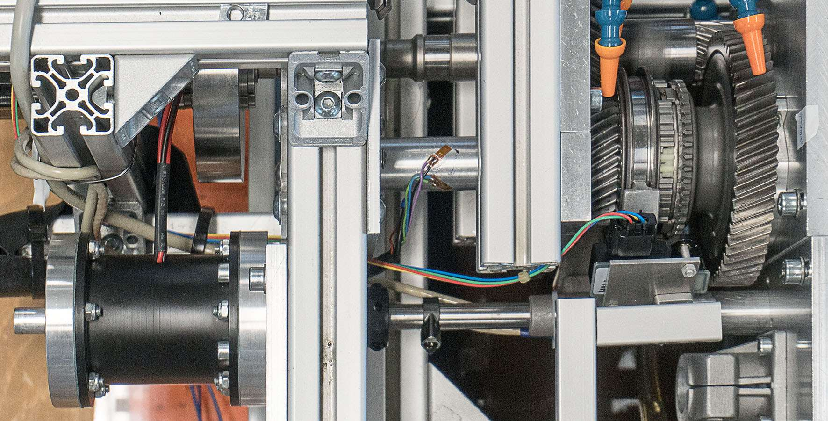
\includegraphics{Bilder/Pruefstand.pdf}
	\caption{Prüfstand \cite[S.5]{adp}}
	\label{fig:Pruefstand}
\end{figure}
\subsection{Getriebe allgemein}

Ein Getriebe ist im Automobil dafür zuständig, die Drehzahl des Motors in ein Drehmoment umzuwandeln, welches die Räder antreibt. Da Motoren nur einen kleinen Bereich von Motordrehzahlen abdecken, werden mehrstufige Getriebe verwendet die verschiedene Raddrehzahlen durch unterschiedliche Übersetzungsverhältnisse bereitstellen können.  Das Einstellen des jeweiligen Ganges kann dabei per Hand (Handschaltgetriebe) oder automatisiert über einen Aktor (Schaltaktorik) erfolgen. 
Im Fahrzeuggetriebe, beispielhaft dargestellt in \autoref{fig:Fahrzeuggetriebe} ist die Eingangswelle, welche durch den Motor angetrieben wird, über eine Zahnradverbindung  fest mit der  Vorgelegewelle verbunden. Auf ihr sind noch weitere fest fixierte Zahnräder angebracht, deren Anzahl mit den verfügbaren Gängen übereinstimmt. Diese greifen jeweils in Losräder auf der Abtriebswelle. Um einen bestimmten Gang einzulegen muss nun das jeweilige Losrad für den Moment fest mit der Abtriebswelle verbunden werden, sodass nur diese Zahnverbindung ein Drehmoment überträgt. Dies geschieht über eine formschlüssige Verbindung mit einer Schaltmuffe, die über die durch den Aktor angetrieben Schaltgabel in Position gebracht wird.

\begin{figure}[h]
	\centering
		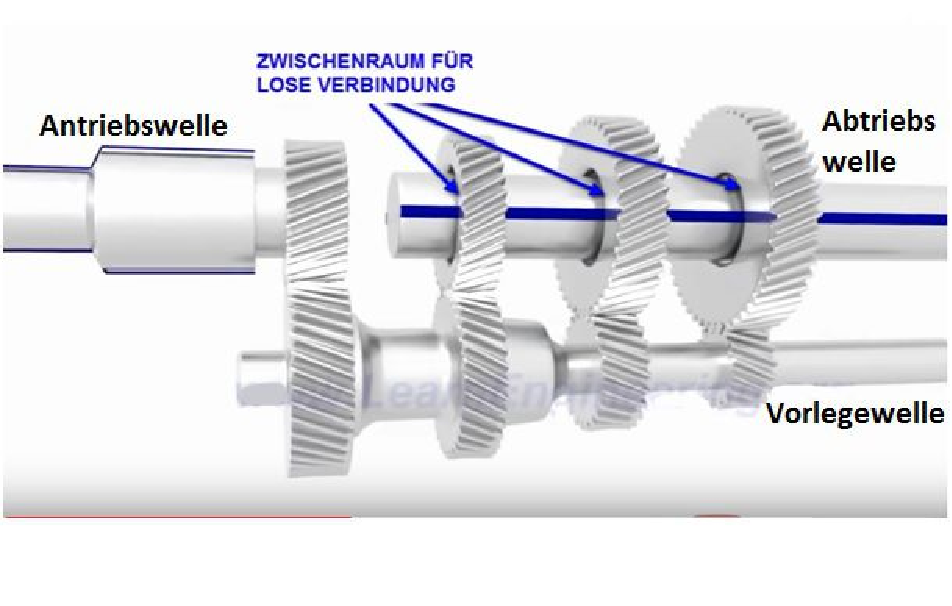
\includegraphics{Bilder/Fahrzeuggetriebe.pdf}
	\caption{Fahrzeuggetriebe}
	\label{fig:Fahrzeuggetriebe}
\end{figure}

\subsection{Getriebe des Prüfstands}

Der Prüfstand besitzt zwei Gänge, in die über eine Schaltgabel geschaltet werden kann. Eine Bewegung der Schaltgabel nach links legt Gang 1 über eine mechanische Synchronisierung ein, während mit Hilfe einer Bewegung nach rechts die Schaltung des Ganges 2 durch eine Klauenkupplung erfolgt. Somit können sowohl Schaltaktoriksysteme mit als auch ohne Synchronring untersucht werden.
Die Bewegung der Schaltgabel wird durch einen Linearaktor ermöglicht, welcher von außen an das Item-Profil verschraubt ist. In diesem ist eine Tauchspule verbaut, die die benötigten Kräfte auf die Läuferstange aufbringt. Über eine starre Wellenkupplung sind Läuferstange und Schaltgabel miteinander verbunden, wodurch die Kräfte auf die Schaltgabel übertragen werden und Schaltvorgänge ermöglicht werden.

\subsection{Aktor}

Der momentan in dem Prüfstand verbaute Tauchspulenaktor wurde von Oliver Hahn im Rahmen seiner Bachelorthesis entwickelt und konstruiert. Er übernimmt im automatisierten Schaltvorgang die Aufgabe, die Schaltgabel  über die Schaltstange translatorisch zu verschieben, welche ursprünglich mit einem Schalthebel per Hand ausgeführt wurde. Die Übertragung des Schaltbefehls an den Getriebeaktor erfolgt dabei durch ein elektrisches Signal (\textit{shift by wire}).
Sein Querschnitt ist in folgender Abbildung schematisch dargestellt.

\begin{figure}[h]
	\centering
		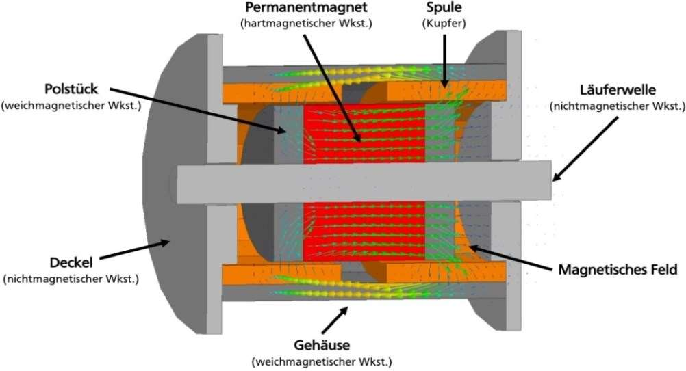
\includegraphics{Bilder/QuerschnittAktor.pdf}
	\caption{Querschnitt Tauchspulenaktor \cite[S.30]{Hahn2018}}
	\label{fig:Querschnitt Aktor}
\end{figure}

Der Aufbau ist zylindrisch und kann in den ortsfesten Stator und den beweglichen Läufer unterteilt werden. Der Stator des Aktors besteht aus zwei in Reihe geschalteten Kupferspulen, welche fest in dem Gehäuse aus Weicheisen liegen und nach oben und unten mit Deckeln aus Aluminium fixiert werden. Der Läufer besteht aus einer nichtmagnetischen Läuferwelle, auf der sich fünf Permanentmagneten aus Neodym-Eisen-Bor befinden, welche mit Hilfe von zwei Polstücken aus Weicheisen axial auf der Läuferstange montiert sind. 
Werden nun die Kupferspulen von Strom durchflossen, so wirkt eine vom Magnetfeld der Permanentmagneten induzierte Lorentzkraft orthogonal auf sie. Diese Kraft ist abhängig von der Stromstärke I, der magnetischen Flussdichte der Permanentmagneten B und der vom Magnetfeld durchsetzten Leiterlänge l:
\begin{equation}\label{eq:lorentz}
F=I\cdot l\cdot B
\end{equation}
Da die Spulen jedoch fest im Gehäuse verbaut sind, wirkt eine entgegengerichtete Kraft auf die Permanentmagneten, die auf der axial verschiebbaren Läuferwelle lagern. Diese Kraft bewirkt dann eine translatorische Bewegung der Welle und somit auch der Schaltgabel. Die Richtung der translatorischen Bewegung kann dabei über die Richtung des in den Spulen fließenden Stromes, der Betrag der Kraft über den Betrag des Stromes eingestellt werden.
Anhand von Abbildung \ref{fig:Kennlinie Aktor} ist zu erkennen, dass die Kraft-Weg Kennlinien des Aktor innerhalb des Nutzungsbereichs von -10 Millimeter bis +10 Millimeter bei verschiedenen Stromstärken annähernd linear verlaufen. 

\begin{figure}[h]
	\centering
		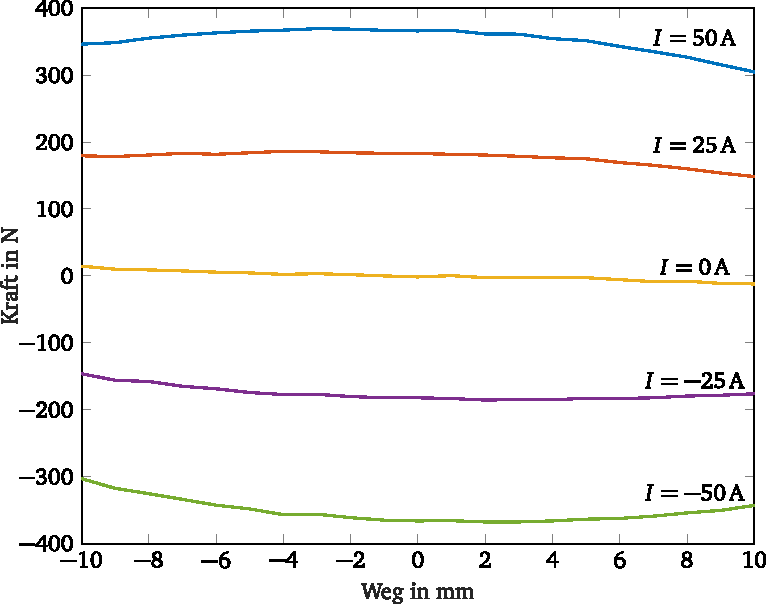
\includegraphics{Bilder/KennlinieAktor.pdf}
	\caption{Kraft-Weg-Strom Kennlinien des Tauchspulenaktors \cite[S.12]{adp}}
	\label{fig:Kennlinie Aktor}
\end{figure}

\subsection{Aktoransteuerung}

Zur Aktoransteuerung wird ein Arduino IBT2 Motortreiber verwendet, die Stromversorgung erfolgt über ein Manson SBC-2130 Battery Charger im Power Supply Mode. Der Motortreiber besteht aus zwei BTS7960 MOSFETs, die je nach Vorgabe des pulsdauermodulierten Signals (PWM-Frequenz) eine Spannung von bis zu 13,8V an den Aktor durchschalten. 

\subsection{Autobox}

Die bisherigen Funktionen am Prüfstand laufen auf einer MicroAutoBox II 1401/1513 der dSpace GmbH. Das Programm zum Schalten des Aktors und der Positionsregelung, welches in MATLAB/SIMULINK entwickelt wurde, wird auf die AutoBox geflasht und diese über die Software dSpace ControlDesk gesteuert.

\subsection {Positionsmessung und -regelung}\label{regler}

Die Position der Läuferstange wird über einen PLCD-25M Sensor gemessen, dessen berührungslose PLCD (permanentmagnetic linear contactless displacement) Technologie die magnetische Sättigung zur Positionsbestimmung verwendet. Der weichmagnetische Kern des Sensors ist über seine komplette Länge von einer Primärspule umgeben. Auf der Schaltgabel ist ein Permanentmagnet befestigt, welcher je nach Position zu einer lokalen Sättigung des weichmagnetischen Kerns führt. Über zwei Auswertungsspulen am Rand des Sensors kann die Position der Sättigungszone entlang der Sensorachse über die induzierte Spannung bestimmt werden.

\begin{figure}[h]
	\centering
		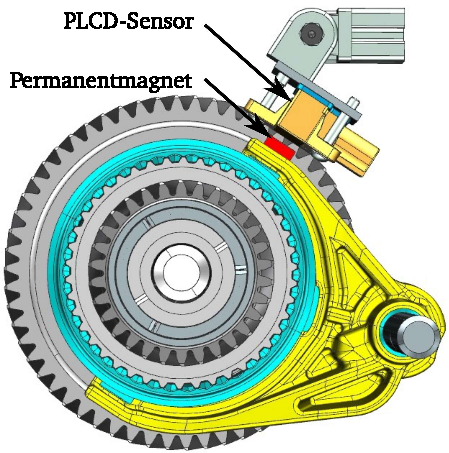
\includegraphics{Bilder/Sensor.pdf}
	\caption{Einbauposition PLCD Sensor an der Schaltgabel \cite[S.14]{adp}}
	\label{fig:Sensor}
\end{figure}
Die Kalibrierung wurde in \cite[S.24f]{messtechnik} entwickelt und erfolgt bisher bei jedem Start. Zu Beginn des Einfahrvorgangs der Schaltwalze wird dabei das Spannungssignal $U\textsubscript{0}$ ausgelesen, welches der Ausgangslage von $x\textsubscript{0}=\SI{0}{mm}$ entspricht. Anschließend werden die Spannungssignale $U\textsubscript{1}$ und $U\textsubscript{2}$ an beiden Anschlägen gemessen. Die Wegdifferenz zwischen den beiden Anschlagspositionen beträgt $x_{ges}$=\SI{16,97}{mm}. Nun kann eine Geradengleichung zur Bestimmung der aktuellen Schaltgabelposition aufgestellt werden. U\textsubscript{a} entspricht dabei immer dem aktuellen Ausgangssignal.

\begin{equation}\label{eq:Lage}
	x=\frac{U\textsubscript{a} -U\textsubscript{0}}{U\textsubscript{1}-U\textsubscript{2}}\cdot x\textsubscript{ges}
\end{equation}

Die bisherige Regelung der Schaltgabelposition wurde in einem vorangegangenem Advanced Design Project ausgelegt. Dazu wurden mithilfe des Ziegler-Nichols-Verfahren zunächst Parameter für einen PID-Regler ermittelt, welcher allerdings noch zu große Totzeiten und ein Überschwingen aufwies. In einer anschließenden iterativen Optimierung mit Störgrößenkompensation wurden die Regelparameter zu $K_P$ =\SI{0,026}{\frac{V}{mm}}, $K_I$ =\SI{0,2}{\frac{V}{s mm}} und $K_D$ =\SI{0,016}{\frac{Vs}{mm}} bestimmt. Der Verlauf der Sprungantwort ist in nachstehender Abbildung (\ref{fig:Sprungantwort Schaltgabelposition}) dargestellt.
\begin{figure}[h]
	\centering
		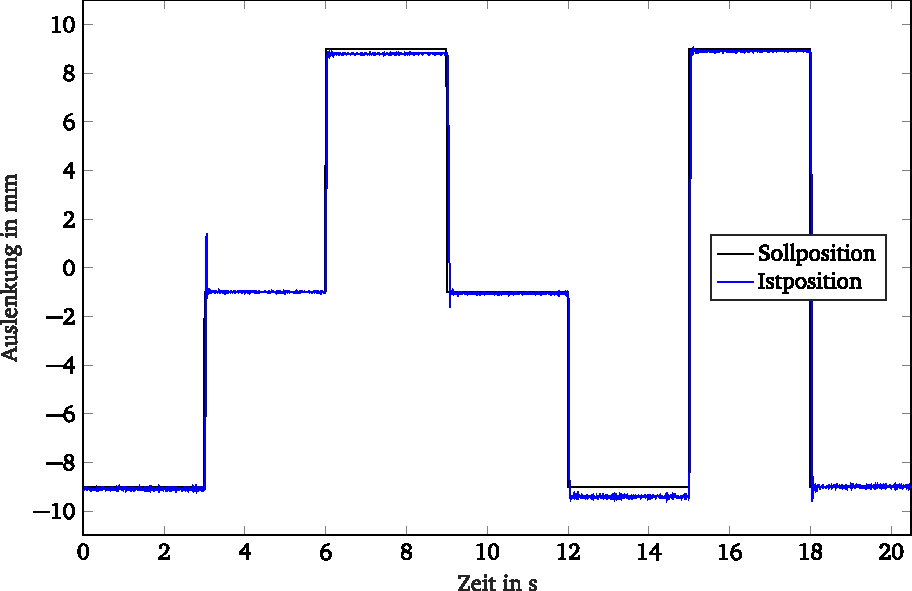
\includegraphics{Bilder/SprungantwortSchaltgabelposition.pdf}
	\caption{Sprungantwort Schaltgabelposition \cite[S.35]{adp}}
	\label{fig:Sprungantwort Schaltgabelposition}
\end{figure}

\section{Grundlagen Löten}
Löten gehört zu den Fügeverfahren und bezeichnet das Verbinden zweier Metalle durch eine Metalllegierung unter Einfluss von Wärme \cite{loeten}. Die Metalllegierung wird dabei als Lot bezeichnet und hat eine geringere Schmelztemperatur (Liquidustemperatur) als die beiden zu verbindenden Metalle (Solidustemperatur). Durch das Löten entsteht eine feste, korrosionsbeständige sowie strom- und wärmeleitende Verbindung. Lötverfahren werden nach Arbeitstemperatur eingeteilt in Weichlöten (bis 450°C), Hartlöten (450°C - 900°C) und Hochtemperaturlöten (über 900°C). Im Rahmen dieses Projektes wird das Verfahren Weichlöten mit Lötkolben angewendet, um die elektrischen Bauteile auf der Platine anzubringen. Dazu können die vom Institut bereitgestellten Lötstationen und –materialien verwendet werden. 

\section{Mikrocontroller}
Ein Mikrocontroller (\textit{MCU: microcontroller unit}) ist ein hochintegrierter Halbleiterchip, der ein komplettes Mikrorechnersystem enthält. Prozessoren, Speicher, Ein- und Ausgabegeräte sind somit auf einem kleinen Chip enthalten der zum Ziel hat, Steuerungs- und Kommunikationsaufgaben möglichst simpel mit wenig Bauelementen zu bearbeiten. 
\begin{figure}[h]
	\centering
		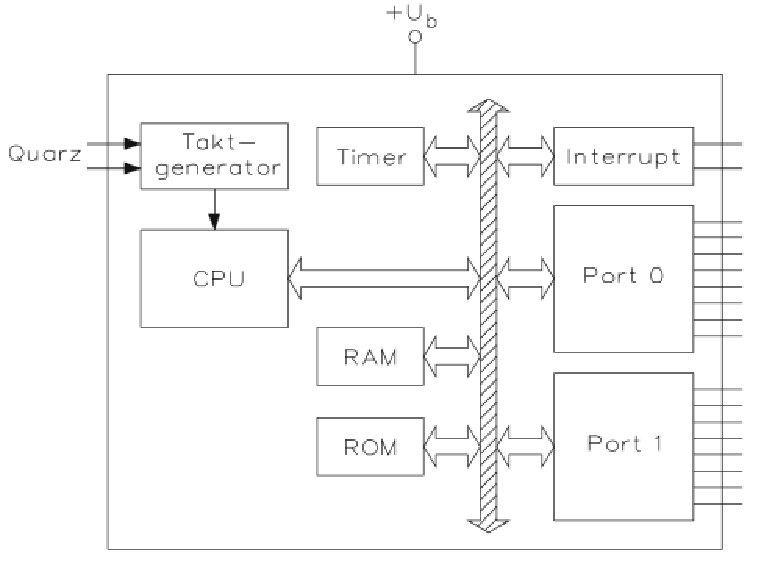
\includegraphics{Bilder/BlockschaltbildMikrocontroller.pdf}
	\caption{Blockschaltbild eines Mikrocontrollers \cite[S.3]{Bernstein2015}}
	\label{fig:Blockschaltbild Mikrocontroller}
\end{figure}

In Abbildung \ref{fig:Blockschaltbild Mikrocontroller} ist der typische Aufbau eines Mikrocontroller dargestellt. Die Schnittstellen zur Peripherie sind durch einen Betriebsspannungsanschluss, einen Takteingang sowie die Portleitungen  gegeben. Bei den Ports wird zwischen Eingangskanälen (\textit{\textbf{I}nput Port}), die digitale Signale lesen, und Ausgangskanälen (\textit{\textbf{O}utput Port}), die digitale Signale setzen beziehungsweise löschen, unterschieden. Des Weiteren können I/O Pins digitale oder analoge Signale auslesen und stellen, wobei analoge Signale mithilfe eines Analog/Digital Wandlers (\textit{ADC}) zuerst in digital Signale umgewandelt werden müssen, damit der Mikrocontroller sie verarbeiten kann.
Eine Spezialform von Eingängskanälen sind die Interrupt-Pins, die bei bestimmten Ereignissen Unterbrechungen des laufenden Programms verursachen, um temporär einen anderen Vorgang zu bearbeiten. 

Intern sind die einzelnen Bausteine, die im folgenden kurz erläutert werden, über ein Bussystem verbunden.
Der Prozessor (\textit{CPU: central processing unit}) führt Berechnungen und logische Operationen durch.
Der Arbeitsspeicher (\textit{RAM: random access memory}) speichert temporär Daten, die aber spätestens nach dem Entfernen der Betriebsspannung verloren gehen.
Der Festspeicher (\textit{ROM: read only memory}) behält seinen Speicherinhalt auch nach dem Entfernen der Betriebsspannung und enthält aufgrund dessen das Programm sowie Einstellungen und wichtige Daten. Im Vergleich zum RAM hat er eine langsame Schreibgeschwindigkeit. 
Ein sogenannter Timer hilft dabei, das Auftreten von Ereignissen zu zählen oder Zeitabstände zu messen, indem beispielsweise Spannungswechsel an einem Eingangskanal gezählt werden. 

Die genaue Ausführung des Chips kann je nach Aufgabentyp variieren, sodass eine Vielzahl an verschiedenen Mikrocontrollern erhältlich ist. Diese unterscheiden sich in der Größe des Speichers, in der Anzahl der Anschlüsse beziehungsweise Schnittstellen, in der Bitbreite, in den Taktraten sowie in der Bauform. Typischerweise werden Mikrocontroller in eingebetteten Systemen (\textit{embedded systems}) verwendet, bei denen die Steuereinheit direkt im System selbst integriert ist. Übliche Anwendungen für Mikrocontroller sind Robotik, Handys, Temperaturregler oder Motorsteuerungen \cite{Brinkschulte}. 

\section{Eingebettete Systeme und Smart Actuators}
Eingebettete Systeme werden definiert als Rechenmaschinen, die für den Anwender weitgehend unsichtbar in einem technischen System eingebettet sind und mit diesem in Wechselwirkung stehen \cite[S.8]{Gessler2014}. Der Rechner kann dabei für Regelungs-, Steuer- oder Überwachungsaufgaben und/ oder für Signal- und Datenverarbeitung zuständig sein. Der allgemeine Zweck ist es, die Stellglieder als Reaktion auf Eingangssignale, die von Sensoren oder manuell vorgegeben werden, zu steuern \cite[S.1]{Broy2003}. Eingebettete Systeme werden oft für speziell eine isolierte Aufgabe entwickelt und angepasst.
Ein Aktor, beziehungsweise Aktuator (aus dem englischen: \textit{actuator}) wird genutzt um elektrischen Signale in eine Bewegung oder Kraft umzusetzen und bildet somit das Stellglied. 
Ein intelligenter Aktor (\textit{smart actuator}) ist definiert als das integrierte Stellglied inklusive aller Komponenten wie Motor, Steuerung, Sensorik und Kommunikationseinheit \cite[S.442]{smartactuator}.
Das Konzept besteht darin, den Aktor um Informationsverarbeitungs- und Kommunikationsmöglichkeiten zu erweitern, sodass der Aktor die eingebettete Elektronik enthält.
Smart Actuators reduzieren beziehungsweise ersetzen die benötigte Interaktion mit einem Menschen oder externen Rechner und können somit effektiver und schneller arbeiten. Außerdem kann oft viel Bauraum eingespart werden, es gibt weniger Komponenten und deutlich weniger Verkabelung, womit der Einbau in ein Gesamtsystem komfortabler ist. Hervorzuheben sind weiterhin die verringerten Kosten, die Überwachung und Diagnose des eigenen Zustands sowie die verbesserte Präzision. Einbußen müssen Smart Actuators allerdings in Bezug auf flexible Anwendungen machen, da sie oft für eine spezielle Aufgabe ausgelegt sind und ihr Verhalten stark vorgegeben ist \cite[S.4]{smartaktor}.


\section{Controller Area Network (CAN)}
Um eine Kommunikation zwischen zwei Geräten (z.B. Sensoren, Aktoren und Steuergeräten) zu ermöglichen, muss ein System zur Datenübertragung vorhanden sein. Dabei hat sich bei vielen PKW- und NKW-Herstellern  das Controller Area Network (CAN) durchgesetzt \cite[S.57]{Werner2014}. CAN ist ein von Bosch für den Automobilbau entwickeltes Bussystem, mit dem mehrere gleichberechtigte Teilnehmer verbunden werden und miteinander kommunizieren können \cite[S. 278]{Woern2006}.
Für ein CAN-Netzwerk werden zwei Leitungen CAN-High und CAN-Low benötigt, an denen alle zu verbindenden Teilnehmer parallel angeschlossen sind. Die beiden Leitungen werden an beiden Enden mit Wellenwiderständen von 120 Ohm verbunden. Der schematische Aufbau eines CAN-Buses mit zwei Teilnehmern ist in Abbildung \ref{fig:CAN} dargestellt. 

\begin{figure}[h]
	\centering
		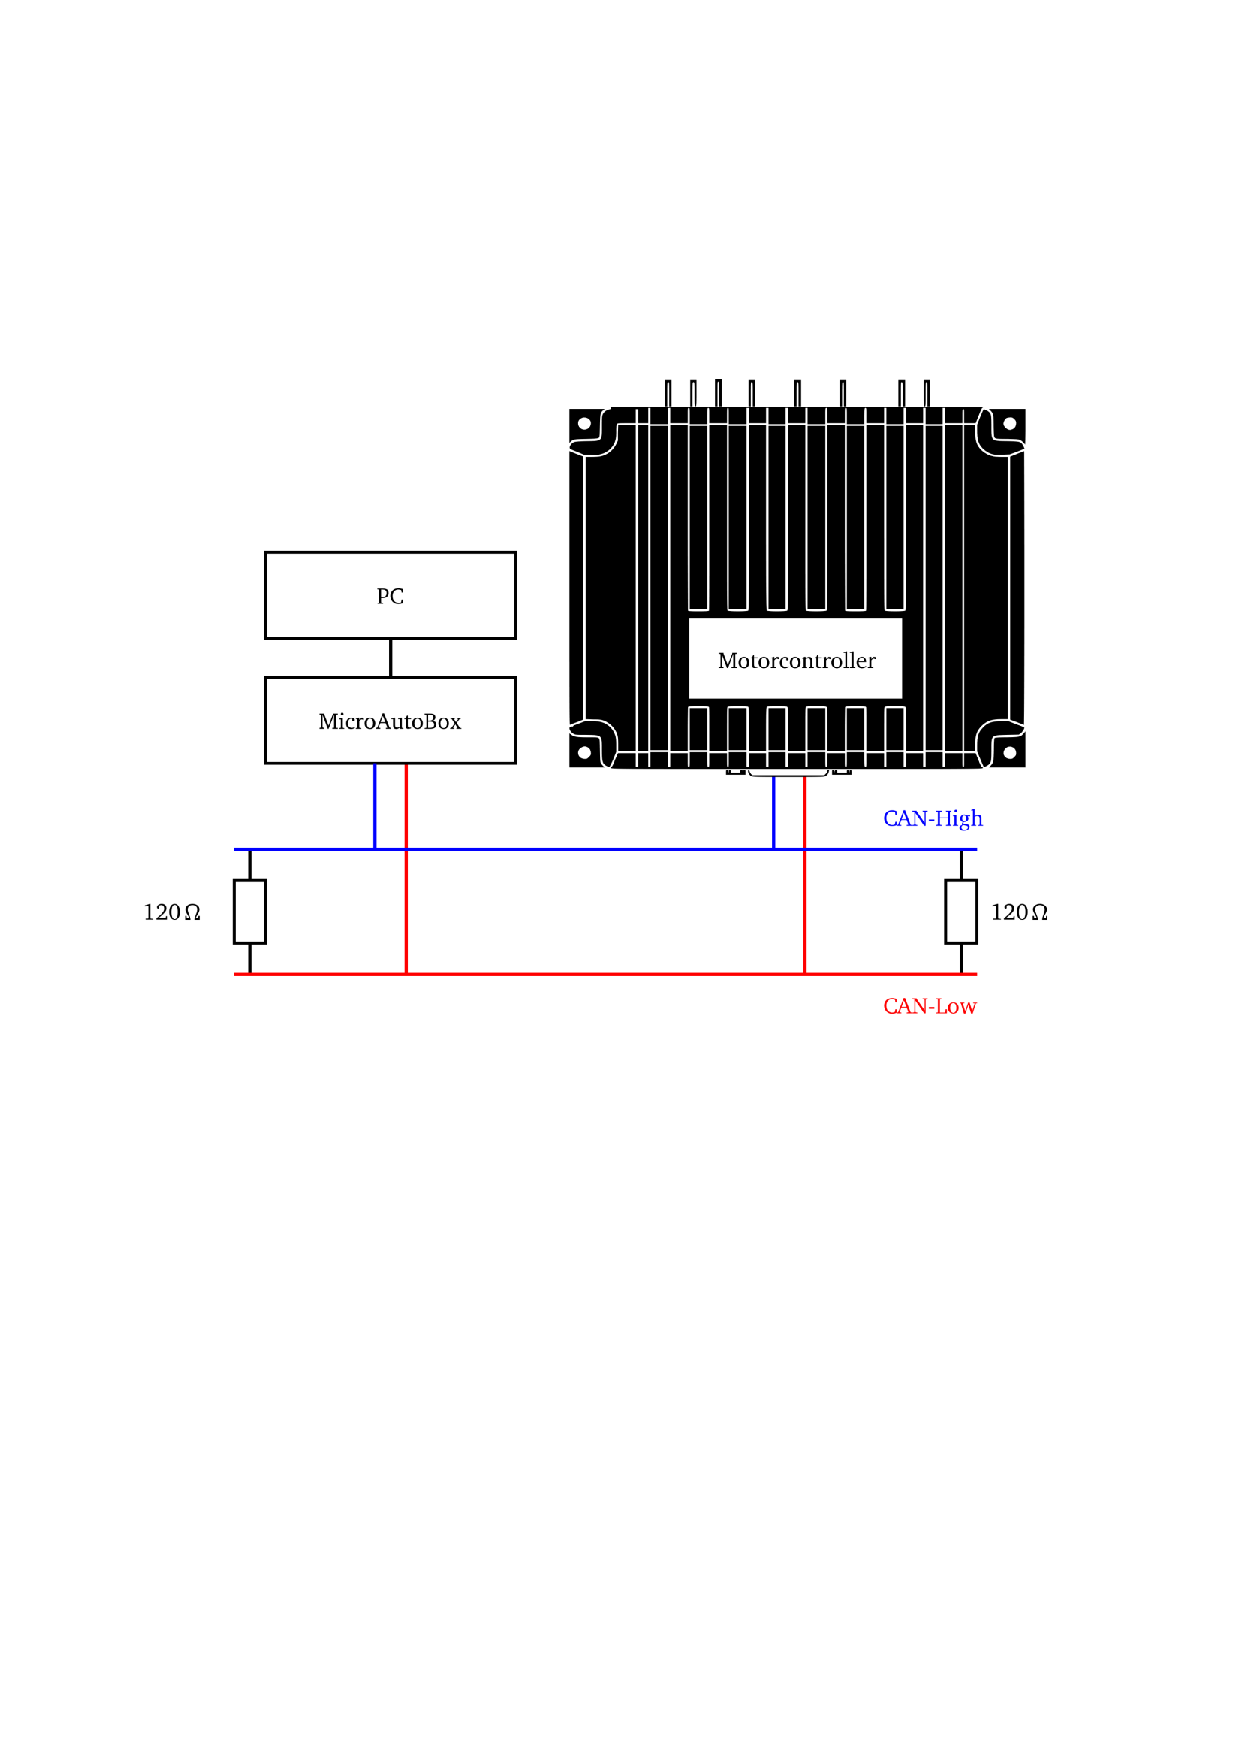
\includegraphics{Bilder/CAN2.pdf}
	\caption{Aufbau CAN-Bus \cite[S.158]{manual}}
	\label{fig:CAN}
\end{figure}

Sollten mehrere Teilnehmer gleichzeitig versuchen eine Nachricht zu senden und somit ein gleichzeitiger Buszugriff vorliegt, kommt es zu einer Kollision. Um diese Aufzulösen wird ein CSMA/CR-Verfahren (\textit{Carrier Sense Multiple Access/Collision Resolution}) verwendet, bei dem die höher gewichtete (dominante) Nachricht die niedriger gewichtete (rezessive) Nachricht überschreibt, sodass der Übertragungsversuch beendet wird. Die Einteilung der Relevanz einer Nachricht erfolgt auf Basis der sogenannten Identifier(ID)-Bits, wobei niedrige ID-Bits eine höhere Relevanz als höhere ID-Bits haben. Dadurch wird eine Hierarchie der Nachrichten erzeugt, wodurch die Nachricht mit der niedrigsten ID immer gesendet werden darf. Dementsprechend werden wichtigen Nachrichten niedrige IDs zugeteilt \cite{Lawrenz2010}. 
Die Geschwindigkeit der Datenübertragung zwischen den Teilnehmer ist dabei von der Länge der Leitungen abhängig und beträgt maximal 1Mbit/s. Nach \cite[S.58]{Werner2014} kann die Bitrate überschlagsmäßig mit 
\begin{equation}
	\text{Buslänge}\leq 40...50 m\cdot \frac{1MBit/s}{Bitrate}
	\label{eq:CAN}
\end{equation}
berechnet werden.

In \autoref{CANNachrichten} wird speziell auf die in dieser Arbeit eingerichtete CAN-Kommunikation eingegangen. Es wird ein CAN-Bus verwendet, mit dem lediglich zwei Teilnehmer miteinander verbunden werden. Diese sind zum einen die MicroAutoBox und zum anderen der Mikrocontroller des Smart Actuators. Die Länge der Leitungen zwischen den beiden ist wesentlich kürzer als 3m, wodurch nach Formel (\ref{eq:CAN}) die maximale Bitrate von 1Mbit/s möglich wird.

\section{Pulsweitenmodulation}
Pulsweitenmodulation (PWM) bietet die Möglichkeit, ein analoges Signal anhand einer digitalen Quelle zu bilden, indem das Tastverhältnis eines Rechteckimpulses bei gleichbleibender Frequenz moduliert wird. Dabei wird der Effekt ausgenutzt, dass sich ein digitales Signal, welches schnell genug und in einem gewissen Tastverhältnis seinen Zustand wechselt, sich verhält wie ein analoges Signal mit konstanter Spannung. So ist es mithilfe von PWM zum Beispiel möglich mit einem Mikrocontroller, der nur einen gewissen Spannungsbetrag liefern kann, verschieden hohe Spannungsignale am Endgerät zu erzeugen um es zu betreiben. Es muss allerdings darauf geachtet werden, dass die Pulse im Endeffekt nicht mehr als einzelne Pulse wahrgenommen werden können, das heißt die Frequenz der Pulse muss höher sein als die Abtastrate des Empfängers.

Das Tastverhältnis, oder der Tastgrad p, beschreibt dabei das Verhältnis zwischen der Einschaltzeit t\textsubscript{ein} und der Periodendauer T:

\begin{equation}
	p=\frac{t\textsubscript{ein}}{T} = \frac{t\textsubscript{ein}}{t\textsubscript{ein}+t\textsubscript{aus}}
\end{equation}

Das Tastverhältnis kann nur Werte zwischen 0 und 1 annehmen.

Der zeitliche Mittelwert der Spannung U\textsubscript{m} ergibt sich dann bei einer Betriebsspannung V\textsubscript{b} zu:

\begin{equation}
	U\textsubscript{m}=V\textsubscript{b}\cdot p
\end{equation}

In Abbildung \ref{fig:PWM} ist ein pulsweitenmoduliertes Signal mit dem entsprechendem zeitlichen Mittelwert aufgetragen. Das Tastverhältnis entspricht hier $p=0,75$.

\begin{figure}
	\centering
		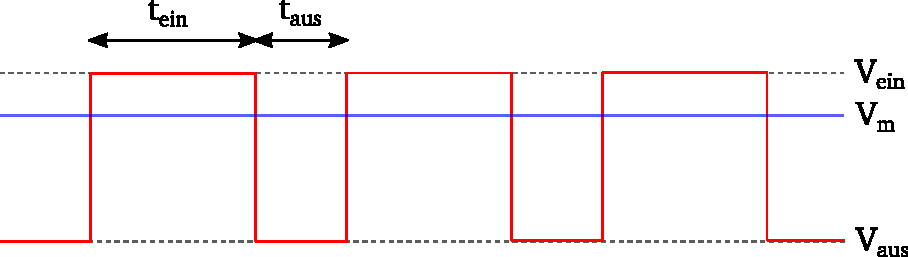
\includegraphics{Bilder/PWM.pdf}
	\caption{Beispielhaftes PWM Signal}
	\label{fig:PWM}
\end{figure}

\section{Zustandsautomaten}
Zustandsautomaten, auch endliche Automaten genannt, eignen sich zur Beschreibung von Systemen, in denen eine endliche Anzahl an Ereignissen eintreten können. In ihnen treten Zustände, Zustandsübergänge und Aktionen auf, aus dem das Verhalten einen Systems modelliert wird. Zustandsübergänge sind logische Operatoren, die erfüllt sein müssen, damit ein System von Zustand X in Zustand Y wechselt. Dementsprechend hat ein Übergang immer einen Zustand als Ein- und Ausgang. Aktionen können durch den Eingang in einen Zustand, den Ausgang aus einem Zustand oder durch eine Eingabe ausgelöst werden. \\
Eine visuelle Darstellung von Zustandsautomaten kann über Zustandsübergangsdiagramme erfolgen. Dabei werden die Zustände mit Pfeilen (Zustandsübergänge) verbunden. Diese Pfeile werden mit Bedingungen beschriftet, die erfüllt sein müssen, damit der Zustand in Richtung des Pfeils gewechselt wird. In den Zuständen selbst stehen die Aktionen die bei Ein- und Ausgang aus dem Zustand, sowie bei bestimmten Eingaben ausgeführt werden.

\section{Serial Wire Debug}
Serial Wire Debug (SWD) ist eine Weiterentwicklung des IEEE-Standards 1149.1 (\textit{JTAG}), welcher eine Debugging- und Programmiermethode für Mikrocontroller oder FPGAs auf Leiterplatten ist. JTAG wurde ursprünglich entwickelt um die Signalkommunikation zwischen mehreren Chips in einem elektronischen System zu überprüfen und wurde dann zunehmend zur Programmierung eingesetzt \cite{swd}. Während JTAG 5 Pins zur Programmierung benötigt (TCK, State Machine Control, Data In, Data Out, Reset) genügen SWD bei den selben Mikrocontroller-Ausgängen zwei Signale (SWCLK, SWDIO). Die geringe Anzahl der Ports basiert dabei auf dem bidirektionalen SWDIO Pin, welcher die Rolle der Data In und Data Out Ports gleichzeitig übernehmen kann \cite{swd}. Unter Debugging versteht man die geführte Ausführung eines Programms, vornehmlich um Fehlerzustände zu lokalisieren. Programmierung bezeichnet den Vorgang, bei dem ein Programm von einer Programmierumgebung auf die Zielhardware übertragen wird. In diesem ADP wird eine SWD-Verbindung aufgebaut um den Mikrocontroller der Platine zu programmieren.

\chapter{Vorgehensweise und Testverfahren}\label{kap3}
Das folgende Kapitel thematisiert, wie während des Projekts vorgegangen wird, welche Entwicklungsmodelle zum Einsatz kommen und welche Testkonzepte angewendet werden.

\section{Entwicklungsmodell}
Sowohl für die Entwicklung eines Softwaresystems als auch für die Entwicklung von Elektronik haben sich Modelle etabliert, die eine Systematik in den Entwicklungsprozess bringen. Dadurch soll eine hohe Qualität des Entwicklungsprodukts sichergestellt werden. 
Unter Qualität, insbesondere bei Softwaresystemen, werden nach \cite{BasSof} bzw. ISO-Norm 25010 \cite{ISO_25010} Eigenschaften verstanden wie Funktionalität, Zuverlässigkeit, Benutzbarkeit, Effizienz und Änderbarkeit.

Für die vorliegende Aufgabenstellung ist ein Softwaresystem zur
\begin{itemize}
	\item Verarbeitung der Sensorik,
	\item Anwendung des Regelgesetzes,
	\item Ansteuerung der Aktorik,
	\item nichtflüchtige Kalibrierung und
	\item selbstständige Fehlererkennung
\end{itemize}
notwendig. Gleichermaßen muss jedoch eine Elektronik entwickelt werden, auf welcher das Softwaresystem ausgeführt wird und durch welche die Schnittstelle zu notwendigen Komponenten hergestellt wird. Um beide Systeme parallel zu entwickeln wird das V-Modell gewählt, das in \autoref{fig_v_modell} dargestellt ist. 



\subsection{Das V-Modell}

\begin{figure}%
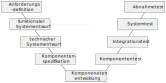
\includegraphics[width=\columnwidth]{./Bilder/fig_v_modell}%
\caption{V-Modell nach \cite{Boehm79}}%
\label{fig_v_modell}%
\end{figure}

Das V-Modell ist ein Vorgehensmodell, dass in verschiedenen Ausführungen existiert. Das hier vorgestellte und angewendete Modell entspricht dem Modell nach \cite{Boehm79}. Als weitere Quelle wird \cite{BasSof} herangezogen und im Folgenden referenziert.
Der linke Zweig stellt dabei die konstruktive Entwicklung dar, während jede Aktivität eine dazu korrespondierende Testaktivität im rechten Zweig besitzt. \\

\subsubsection{Konstruktive Entwicklung (linker Zweig)}
Zunächst wird demnach eine Anforderungsliste im Zuge der \textit{Anforderungsdefinition} erstellt, die die Entwicklungsaufgabe genauer spezifiziert und später eine Überprüfungsgrundlage bietet inwiefern das fertige Gesamtsystem des Wunschsystems entspricht. Daran anschließend wird ein \textit{funktionaler Systementwurf} durchgeführt. Hierbei werden die Anforderungen in Funktionen überführt, die das Gesamtsystem erfüllen muss, um den Anforderungen gerecht zu werden. Darauf folgend findet der \textit{technische Systementwurf} statt. Dafür wird das System in unabhängige Teilsysteme unterteilt und Schnittstellen zur Umwelt ermittelt. Daran logisch anknüpfend wird die \textit{Komponentenspezifikation} durchgeführt. Dafür wird für jede Komponente (elementares Teilsystem) die Aufgabe, das gewünschte Verhalten und Schnittstellen zu anderen Teilsystemen definiert. \\
Den letzten reinen Entwicklungsschritt bildet die \textit{Komponentenentwicklung}. Dabei werden schließlich die einzelnen Komponenten nach der zuvor erarbeiten Spezifikation entwickelt. Eine Komponente stellt dabei ein Teilsystem dar, das eine feste Funktion erfüllt, und in der Regel aus einem Softwareteil und einem Hardwareteil besteht. Beide Teile werden parallel in genauer Abstimmung entwickelt, da die gewünschte Funktion nur durch beide Systeme im Zusammenspiel erfüllt werden kann. Das Softwaresystem besteht dabei in der Regel aus einem Treiber, der die komplexe Hardwareschnittstelle für das Restsystem versteckt und komfortable Schnittstellen bereitstellt. Ein Beispiel dafür stellt der Treiber für den Tauchspulenaktor dar, der eine Pulsweite in Prozent und ein Aktivierungssignal entgegen nimmt. Intern werden dann daraus Steuersignale für die Halbbrücken generiert und über die Elektronikschaltung dem Aktor zugeführt.
Neben Elektronikschaltungen mit zugehörigem Treiber existieren auch \textit{reine Softwarekomponenten}, die unabhängig der Elektronik entwickelt werden wie bspw. eine Verhaltenslogik für ein- und ausgehende CAN-Nachrichten. Ebenso existieren \textit{reine Elektronikkomponenten}, die keinen direkten Bezug zur Software aufweisen und daher unabhängig zur Software entwickelt werden können.\\

\subsubsection{Testaktivitäten (rechter Zweig)}
Alle folgenden Informationen sowie detaillierte Ausführungen bezüglich des Testverfahrens können \cite{BasSof} entnommen werden.\\
Nachdem die Entwicklung aller Komponenten abgeschlossen ist, müssen die einzelnen Komponenten auf die geforderte Funktionalität überprüft werden. Dazu wird jede Komponente so isoliert wie möglich vom Restsystem getestet, ggf. unter Einsatz sogenannter Testtreiber und Platzhalter, um die zu testenden Komponenten mit Testdaten oder Testfällen auszuführen. Durch die Isolation wird sichergestellt, dass die einzelne Komponente als solche funktioniert und Fehlerzustände leichter eingegrenzt und lokalisiert werden können. Jeder Testfall enthält dabei feste Vorbedingungen, Eingabewerte und ein gefordertes Sollverhalten bzw. geforderte Ausgabewerte. Die Auswahl der Testfälle wird durch die Art der Komponenten unterschieden. \textit{Treiber mit zugehöriger Hardwarekomponente} bieten Schnittstellen, die beliebige Zahlenwerte und Kombinationen entgegen nehmen. Daraus resultiert eine quasi unendliche Menge an möglichen Testfällen, die nicht praktikabel getestet werden können. Vollständiges Testen ist daher nicht möglich. Aus diesem Grund werden die Testfälle aus einem Klassifikationsbaum mit anschließender Grenzwertanalyse gewonnen. Dabei wird jeweils mindestens ein Testwert aus jeder Gruppe ausgewählt. Die Gruppierung wird so vorgenommen, dass von jeder Gruppe aus Testwerten gleiches Verhalten angenommen wird. Als Beispiel kann wieder die Ansteuerung des Tauchspulenaktors herangezogen werden. Es wird davon ausgegangen, dass alle Werte zwischen -100 und 0 eine Bewegung in eine feste Richtung bewirken. Dagegen bewirken Werte von 0 bis 100 eine Bewegung in die Gegenrichtung. Werte außerhalb des Zahlenbereichs werden auf entsprechend -100 oder +100 abgerundet. Durch eine Grenzwertanalyse werden diese Gruppen (auch Äquivalenzklassen genannt) noch in Untergruppen unterteilt, in denen die oft kritischen Grenzwerte (-100, 0 und 100) noch eigene Gruppen bilden. Eine Sonderstellung besitzt die Null, weil hier keine Reaktion erwartet wird. Durch kombinatorische Paarbildungen werden darüber hinaus auch beliebige Kombinationen aus abhängigen Eingangswerten, bspw. Aktivierungssignal (enable) und Pulsbreite (PWM [\%]), berücksichtigt. Um die Testfallgenerierung durch Klassifikationsbäume zu verdeutlichen, ist in \autoref{fig_klass} der Klassifikatiosbaum grafisch dargestellt. Die untere Zeile aus konkreten Werten stellt beispielhafte Testwerte aus der darüberliegenden Äquivalenzklasse dar. Darunter ist über die Gitterstruktur angedeutet wie aus der paarweisen Kombination der einzelnen Testwerte Testfälle bestimmt werden. \textit{Testfall 1} entspricht dem Aufrufen des Treibers mit einer PWM von \SI{-100}{\%} und einem aktivierten \textit{enable}-Signal. Es wird daher erwartet, dass der Aktor voll in \glqq negative\grqq{} Bewegungsrichtung bestromt bzw. beschleunigt wird. Ob die Elektronik als solche den Erwartungen bzw. der Spezifikation entspricht, kann durch Strom-/Spannungs- sowie Temperaturmessungen verifiziert werden. 
\begin{figure}%
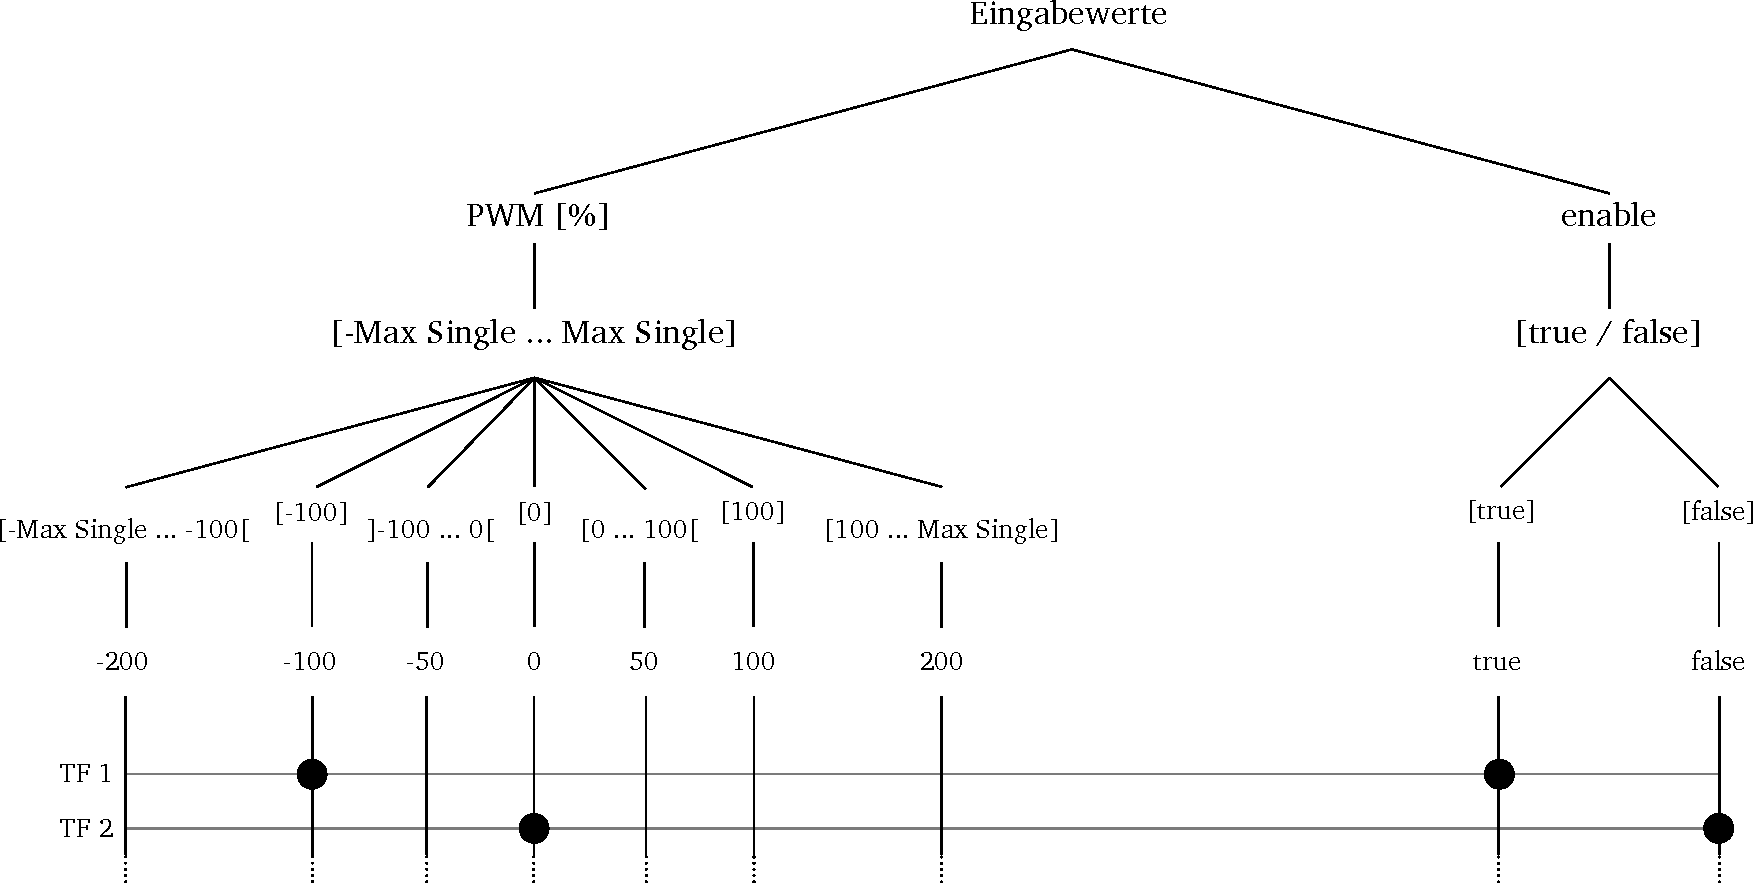
\includegraphics[width=\columnwidth]{./Bilder/fig_klass}%
\caption{Klassifikationsbaum am Beispiel des Motortreibers}%
\label{fig_klass}%
\end{figure}
\\
Für \textit{reine Softwarekomponenten} hingegen werden Testfälle auf eine geeignetere Weise generiert. Bei Softwarekomponenten auf Basis eines Zustandsautomaten werden Testfälle aus einer zustandsbasierten Testfallgenerierung gewonnen. Dabei wird als Testziel vorausgesetzt, dass alle Entscheidungen (Kanten) eines Zustandsautomaten mindestens einmal ausgeführt werden, was als Entscheidungsüberdeckungskriterium bezeichnet wird. Dieses Kriterium schließt auch automatisch ein, dass alle Zustände (Knoten) besucht worden sind. Wie viele Testfälle getestet werden müssen hängt dabei stark von der Größe und Komplexität des Zustandsautomaten ab.\\
Nach dem Test der einzelnen Komponenten wird eine Integration vollzogen. Unter Integration versteht man dabei das Zusammenführen der Komponenten zu einem Gesamtsystem. Es stehen viele Varianten zur Verfügung, dazu zählen \textit{Bottom Up}-, \textit{Top Down}- und \textit{Big Bang}-Integration. Letztere Variante sieht vor, dass alle Komponenten in einem Zug ins Gesamtsystem integriert werden. Auftretende Fehler können jedoch in diesem Fall nur schwierig zugeordnet werden. Günstiger ist daher die \textit{Bottom Up}-Integration, wobei nach und nach Komponenten hinzugefügt werden und übergeordnete Komponenten, die mit mehreren Einzelkomponenten Schnittstellen haben, später integriert werden. Da im vorangehenden \textit{Komponententest} bereits die Komponenten getestet sind, ist im anschließenden \textit{Integrationstest} mit Fehlern zu rechnen, die durch Schnittstellen zwischen den Komponenten hervorgerufen werden. Es kann davon ausgegangen werden, dass die Komponenten intern funktionieren und ausschließlich das Zusammenspiel der Komponenten fehlerhaft ist. \\
Zuletzt entsteht somit ein Gesamtsystem, das darauf getestet werden muss, ob die im \textit{funktionalen Systementwurf} festgelegten Funktionen erfüllt werden. Um dies zu testen werden \textit{Use-Case}-Szenarios erstellt, die eine übliche Nutzung simulieren. Dabei wird von mehreren Akteuren ausgegangen, die mit dem System in der realen Anwendung agieren werden. Der Schaltaktor wird bspw. über ein übergeordnetes Steuergerät (\textit{electrical Control Unit}) angesteuert. Die Schnittstelle wird durch CAN realisiert, sodass ein entsprechendes Steuergerät über CAN Signale/Befehle einen Schaltvorgang anfordern kann oder eine Fehlermeldung auslesen kann. Einen typischen \textit{Use-Case} würde bspw. ein Schaltbefehl vom neutralen in den zweiten Gang darstellen. Dieser kann erfolgreich ablaufen oder durch eine mechanische Blockade verhindert werden. Abschließend erfolgt der Abnahmetest, der in der Regel durch den Auftraggeber durchgeführt wird. Hier wird explizit verglichen, ob die versprochenen Leistungen im Pflichtenheft auch erreicht werden.

Diese und weitere Informationen für den interessierten Leser finden sich in \cite{BasSof}.

\subsection{Konkretes Vorgehen mit inkrementellem Entwicklungsansatz}

Neben dem V-Modell fließen auch inkrementelle Ansätze in die Entwicklung ein. So wird das V-Modell mehrmals durchlaufen, während nach jeder Iteration ein ausführbares und testbares Entwicklungsprodukt vorliegt. Diese Zwischenprodukte entsprechen der Anforderungsliste unter Umständen nur teilweise, sodass mehrere Iterationen bis zu einem zufriedenstellenden Produkt notwendig sind. Für das vorliegende Projekt wird in der ersten Iteration ein Prototyp angestrebt, der bereits die Grundfunktionalitäten bereitstellt. Dies umfasst die Möglichkeit, einen Schaltvorgang nach Anforderungsspezifikation durchzuführen. Dafür muss unter Anderem die Aktorik ansteuerbar sein und die Sensorik notwendige und hinreichend genaue Regelgrößen liefern. 
Während der Phase des Prototyping wurde der Mikrocontroller auf einem Entwicklungsboard verwendet, um Daten über die USB-Schnittstelle mit dem PC austauschen zu können, über die der Mikrocontroller auch programmierbar ist, und alle Pins leicht über Stiftleisten erreicht werden können. Die Funktionalität der geplanten Brückenschaltung zur Aktorsteuerung wurde dafür zunächst unabhängig vom Aktor getestet, um seine Sicherheit zu gewährleisten. Dies wurde der Einfachheit halber auf Steckbrettbasis und mit Anschluss zweier LEDs statt dem Motor durchgeführt. Die PWM-Frequenz konnte dabei die Helligkeit der LEDs steuern und durch verschiedene Eingangssignale in die schaltenden Transistoren wurde vorgegeben, welche der beiden LEDs leuchten soll. Um für den ersten Prototypen mit dieser Schaltung den Aktor anzusteuern, wurde der Leistungsteil mit THT-Bauteilen (\textit{through hole technology}-Bauteilen) auf eine Lochrasterplatine gelötet, da durch ihn größere Ströme als für Steckbrett empfohlene 1 Ampere fließen.
Die Elektronik für den Lagesensor, welcher bereits von Vorgängerprojekten genutzt wurde, wird ebenfalls auf einem Steckbrett realisiert. Um den Prototypen schließlich in Aktion zu testen, wird ein Testprogramm geschrieben und auf den Mikrocontroller geflasht. Anforderungen an Größe, Effizienz oder Integrierbarkeit sind bei diesem ersten Prototypen nicht verfolgt worden. Durch das Ergebnis werden Erkenntnisse gewonnen, die in den nächsten Iterationen berücksichtigt werden. 
Bei folgenden Iteration wird versucht über geeignete Maßnahmen (bspw. durch eine angepasste Komponentenspezifikation) bisherige Ergebnisse zu verbessern und weitere Anforderungen zu erfüllen. 
Hierfür rückt besonders die iterative Weiterentwicklung der Software in den Vordergrund, da fast die komplette benötigte Hardware zur Anforderungserfüllung bereits im ersten Prototypen Anwendung findet. %Nichtflüchtige Kalibrierung/ CAN etc%
Im nächsten Schritt wurde an der automatischen Fehlererkennung gearbeitet. Um Strommesswerte zu erhalten wurde, musste die integrierte Strommessung der verwendeten Halbbrücken über den Statuspin vom Mikrocontroller ausgelesen werden. Zur Erkennung von Übertemperatur im Aktor wird ein externer Temperatursensor angeschlossen und ausgelesen.
Einen wesentlichen Iterationsschritt stellt schließlich der Übergang von Steckbrett- auf Platinenbasis dar. Durch diesen Übergang treten weitere Anforderungen wie Baugröße und Integrierbarkeit in den Vordergrund. Nach dem letzten Iterationsschritt sollten alle Anforderungen nachweislich erfüllt sein, sodass ein erfolgreicher System- und Abnahmetest durchgeführt werden kann. In \autoref{fig_entw_evo} sind die Iterationen exemplarisch dargestellt, während in \autoref{tab_entw_evo} ein beispielhafter Ausschnitt aus dem Ergebnis des jeweiligen \textit{Systemtests} pro Iteration dargestellt sind.

\begin{table}%
\centering
\captionabove{Beispielhafter Ausschnitt aus Systemtest-Ergebnissen über mehrere Iterationen}
\begin{tabular}{c c c c c c c}
Iteration & Schaltzeit & Nichtflüchtige Kalibrierung & kompakte Baugröße & Effizienz & Fehlererkennung & ...  \\
\hline
1 & \checkmark  & \checkmark & \texttimes & \texttimes & \texttimes & ...  \\
2 & \checkmark & \checkmark & \texttimes & \texttimes & \checkmark  & ...   \\
3 & \checkmark & \checkmark & \texttimes & \checkmark & \checkmark  & ...   \\
...    \\
\end{tabular}
\label{tab_entw_evo}
\end{table}

\begin{figure}%
\centering
\includegraphics[width=0.7\columnwidth]{./Bilder/fig_entw_evo}%
\caption{Bildliche Darstellung des Prototypings (Iterationsprozesses)}%
\label{fig_entw_evo}%
\end{figure}

\chapter{Auswahl elektronischer Komponenten und Verschaltung}\label{ch:komp}
Im Folgenden wird auf die Auswahl der Platinenkomponenten, sowie deren Beschaltung eingegangen. Der gesamte Schaltplan ist in \autoref{app:boardlayout} angefügt.
\section{Anforderungen an die Komponenten}
Elektronische Komponenten sind üblicherweise in passive und aktive Bauelemente untergliedert. Unter passiven Bauelementen werden Komponenten verstanden, die das Eingangssignal ohne Verstärkung übertragen. Aktive Bauelemente benötigen meist eine Hilfsquelle und können somit ein Eingangssignal verstärken \cite[S.25]{haendschke}. Für den Einsatz elektronischer Komponenten im Automobilbereich hat sich für passive Bauteile die Zertifizierung nach AEC-Q200 und für aktive Bauteile nach AEC-Q100 als Qualitätsstandard etabliert. Anhand dieser Zertifizierungen wird eine nachweisliche Belastbarkeit der Bauelemente nach dem jeweiligen Standard definiert. Für die Anforderungen an die Platine werden die passiven Bauelemente nach AEC-Q200 und die aktiven Bauelemente nach AEC-Q100 mindestens in \textit{Grade 2} eingestuft, um den Temperaturanforderung bis \SI{105}{^\circ C} gerecht zu werden \cite[S.6]{aecq}. 
\subsection{Passive Bauteile}
Unter die benötigten passiven Bauteile fallen Kondensatoren und Widerstände, welche nach dem AEC-Q200 Standard ausgewählt werden. Anforderung ist danach eine thermische Belastbarkeit von mindestens \SI{105}{^\circ C}. Um eine geringe Baugröße der Platine zu gewährleisten, sollten sowohl Widerstände als auch Kondensatoren als SMD (\textit{surface-mounted device}) gekauft werden. Für Abblockkondensatoren werden nach \cite[S.7]{ldo} Keramikkondensatoren mit XR7 präferiert. Diese werden einerseits dazu genutzt, um bei impulsartiger Netzbelastung durch hohe Leistungsaufnahme von ICs das Netz zu entlasten, andererseits aber auch um Restwelligkeiten zu filtern. Als Baugröße bei manueller Bestückung bieten sich die Standardgrößen 1206 oder 0805 (Angabe in $\frac{1}{100}$ Zoll), welche noch per Hand lötbar sind. Die Widerstände für die Sensorik müssen mit sehr hoher Präzision, geringem Rauschen und niedriger Temperaturabhängigkeit gewählt werden, um Messfehler aufgrund falscher Widerstandswerte zu vermeiden. Im Anwendungsfall bieten sich daher Dünnschichtwiderstände an.
\subsection{Aktive Bauteile}
Die aktiven Bauelemente der Platine müssen dafür ausgelegt werden, um im späteren alle Anforderungen aus der Anforderungsliste gerecht zu werden. Demnach müssen sie in ihrer logischen Verschaltung einerseits in der Lage sein den Tauchspulenaktor anzusteuern und auszuregeln, andererseits aber auch die Bedingungen über Leistungsaufnahme etc. erfüllen. Kern der Platine ist ein Mikrocontroller, welcher schnell genug sein muss, um Gangwechsel in weniger als \SI{0,1}{s} durchzuführen. Weiterhin muss der Mikrocontroller die CAN-Kommunikation mit der MicroAutobox unterstützen. Da der Mikrocontroller nicht über die \SI{13,8}{V} der Autobatterie gespeist werden kann, wird ein Spannungsregler benötigt, welcher auf die Betriebsspannung des Mikrocontrollers regelt. Um aus den physikalischen Bussignalen CAN-HIGH und CAN-LOW für den Mikrocontroller verwertbare Signale zu erhalten wird ein CAN-Transciever benötigt. Über diesen ist eine Kommunikation des Mikrocontrollers mit der CAN-Peripherie erst möglich. Zum Regeln des Tauchspulenaktors ist ein Motortreiber nötig, welcher vom Mikrocontroller angesteuert wird, um die Spannung an den Tauchspulenaktor durchzuschalten. Eine Ansteuerung des Motortreibers mittels PWM-Signal sollte möglich sein. Der Motortreiber muss dabei für zukünftige Aktorkonfigurationen für Ströme bis zu \SI{55}{A} ausgelegt sein. Des Weiteren wird eine Spannungsebene von \SI{5}{V} benötigt um die Lagesensorik des Aktors zu unterstützen, wofür ein zweiter Spannungsregler eingeplant werden muss.
%\begin{figure}[H]%
%\centering
%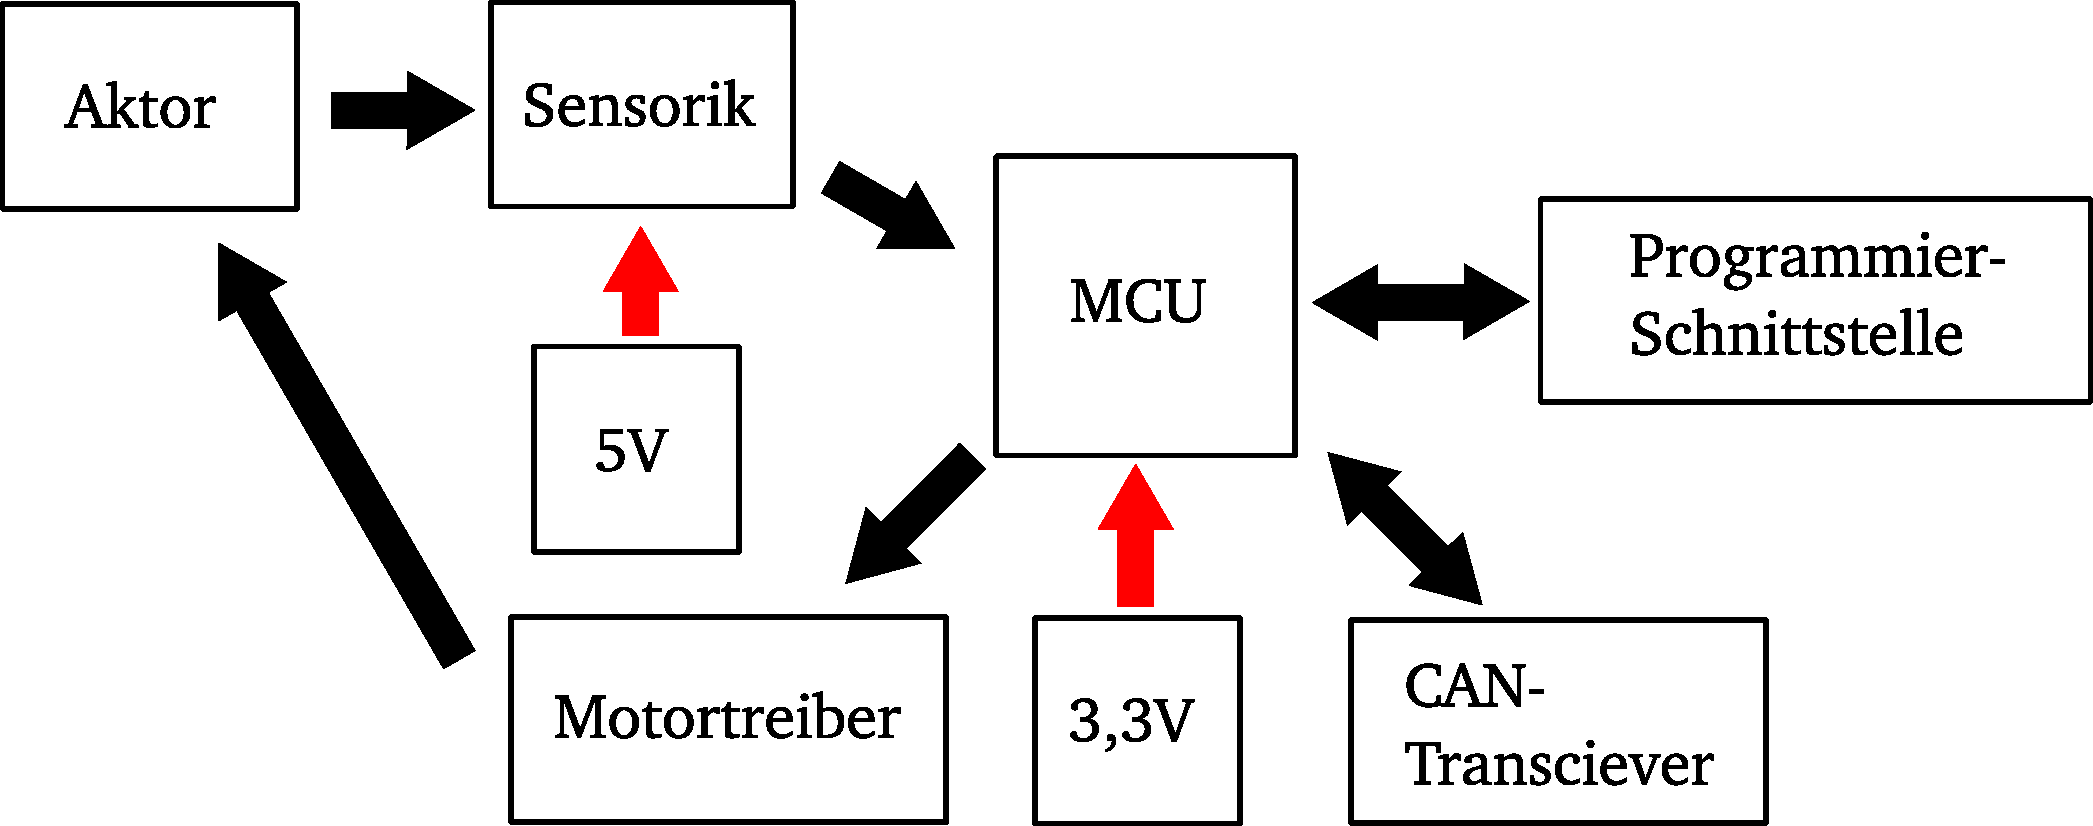
\includegraphics[width=250pt]{./Bilder/anf.pdf}%
%\caption{Benötigte Ebenen der Verschaltung}%
%\label{fig:anf}%
%\end{figure}
\newpage
\section{Komponentenauswahl}
Anhand der Anforderungen an die Platinenelemente sind die endgültigen Komponenten der Platine zu wählen. Es müssen Mikrocontroller, Spannungsregler, CAN-Transciever und Motortreiber ausgewählt werden. Weiterhin wird eine Temperaturbeständigkeit bis \SI{105}{^\circ C} gefordert.
\subsection{Mikrocontroller}
Die Recheneinheit zur Regelung des Tauchspulenaktors ist ein STM32F405RGT7-Mikrocontroller. Dieser ist mit verschiedenen Pin-Anzahlen erhältlich und auf der Platine aus Platzgründen in der Ausführung LQFP64 mit 64 Pins verbaut. Der Mikrocontroller zeichnet sich durch seine hohe CPU-Geschwindigkeit von \SI{168}{MHz} und seine große Programm-Speichergröße von \SI{1}{MB} aus. Die Namensendung -T7 steht dabei für die zulässige Betriebstemperatur von -40...\SI{105}{^\circ C}. Weiterhin besitzt dieser Mikrocontroller die geforderten CAN-Schnittstellen, anhand derer mit der MicroAutobox kommuniziert werden soll. In \autoref{fig:mcumin} ist die Minimalbeschaltung des Mikrocontrollers zu sehen. Diese ist dem Datenblatt des STM32 entnommen \cite[S.77]{stm32}. Die Pins mit den Bezeichnungen VDD...VDD\_4 sind die Versorgungspins des Mikrocontrollers. An diesen Pins liegt die Versorgungsspannung an, welche nach dem Datenblatt zwischen 1,8 und \SI{3,6}{V} liegt. Diese ist aufgrund der Versorgungsspannung anderer Bauteile zu VDD = \SI{3,3}{V} gewählt. Die VDD Pins werden durch die Keramikkondensatoren C7 bis C11 entkoppelt, welche nach dem Datenblatt dimensioniert sind und möglichst nah an den dem jeweiligen VDD-Pin plaziert werden sollen. Die Entkopplung wird benötigt, um Welligkeiten der Spannungsversorgung zu filtern und parasitäre Induktivitäten zu entkoppeln \cite{decoupling}. Der Pin VBAT wird unter Anderem für die Versorgung der Echtzeituhr (\textit{RTC}), der Backup-Register und des Backup-SRAMs genutzt und wird, wenn keine zweite Spannungsversorgung neben der Hauptversorgung vorhanden ist, ebenfalls an VDD angeschlossen \cite[S.31]{stm32}. VDDA ist der Pin für die Spannungsversorgung des Analog-Digital-Converters (\textit{ADC}) und wird ebenfalls mit der Versorgungsspannung von VDD angeschlossen. Die Kapazitäten C5 und C6 sind nach den Herstellerangaben dimensioniert und sorgen ebenfalls für eine Entkopplung der Spannungsversorgung. Die Induktivität L1 bietet die Möglichkeit, je nach Welligkeit der Versorgungsspannung, diese über einen LC-Filter zu filtern um eine bessere Auflösung des ADCs zu gewährleisten. Wenn dieser Filter nicht benötigt wird, sollte L1 durch einen \SI{0}{\Omega} Widerstand ersetzt werden.
VCAP\_1 und VCAP\_2 sind die Ausgänge des internen Voltage Regulators des STM32 und C5 bzw. C6 werden zur Glättung der intern geregelten Spannung genutzt \cite[S.77]{stm32}. Die Pins VSS, VSS\_2 und VSSA sind die GND Anschlüsse für den Mikrocontroller und den internen ADC.
\begin{figure}[H]%
\centering
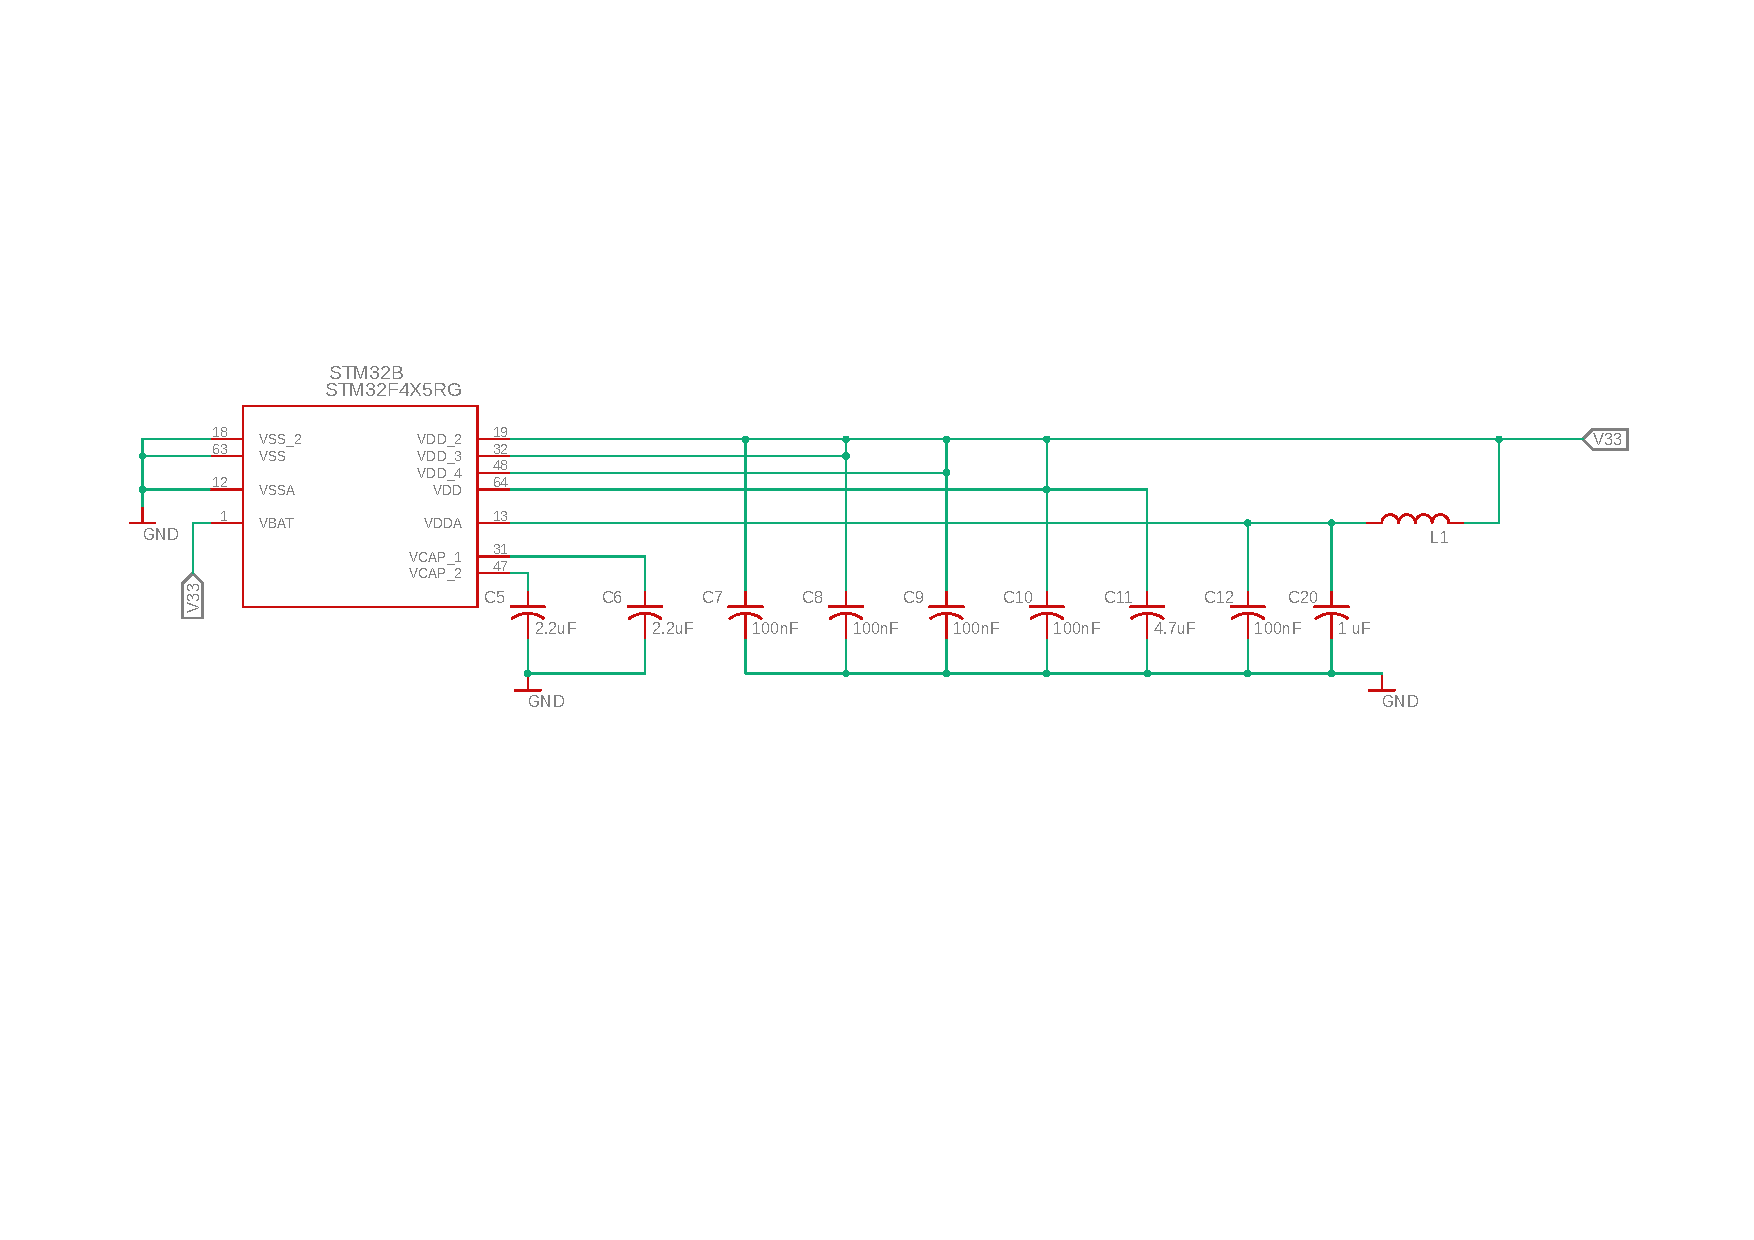
\includegraphics[width=\columnwidth]{./Bilder/MCU_MIN.pdf}%
\caption{Minimalbeschaltung des STM32F405RGT7}%
\label{fig:mcumin}%
\end{figure}\noindent
In \autoref{fig:mcupin} sind die Pin-Belegungen des Mikrocontrollers dargestellt, welche durch \autoref{tab:pins} genauer beschrieben sind. Unter Sensorik fallen die Ausgänge für Lagesensorik, Temperatursensorik und Messung der Versorgungsspannung. Die UART Pins können zum \textit{debuggen} auf der endgültigen Platine genutzt werden. Zur CAN-Kommunikation werden die Pins CAN1-TX (PA11) und CAN1-RX (PA12) benötigt, womit der Mikrocontroller über einen CAN-Transciever Nachrichten an die MicroAutobox senden und ebenfalls Nachrichten von dieser empfangen kann. Zum Programmieren des Mikrocontrollers wird eine \textit{SWD}-Schnittstelle aufgebaut, welche sich mittels externem ST-Link/V2 mit dem Computer verbinden lässt. Dazu werden die jeweiligen Pins über den Platinenstecker nach außen geführt (vgl. \autoref{fig:stecker}). Weiterhin müssen Pins zum Beschalten der H-Brücke und zum Auslesen der Strommessungen belegt werden. Die Pins OSC\_IN und OSC\_OUT sind zum Anschließen eines externen Quarzes, welcher als Taktgeber für den Mikrocontroller genutzt wird. Der Pin NRST wird für den Fall eines notwendigen Resets herausgeführt. Über diesen kann der Mikrocontroller bei Fehlern im Befehlszähler (\textit{program counter corruption}) wieder in den Initialzustand des Programms zurückgesetzt werden. Daten aus dem Flash-Speicher bleiben dabei unverändert. Dazu muss der NRST-Pin für eine Sekunde extern auf \textit{low} (0 bis \SI{0,8}{V}) gezwungen werden \cite[S. 111]{stm32}. Somit ist im Falle eines undefinierten Programmzustands auch im eingebauten System ein Programmneustart möglich.

\noindent\begin{minipage}{0.75\textwidth}
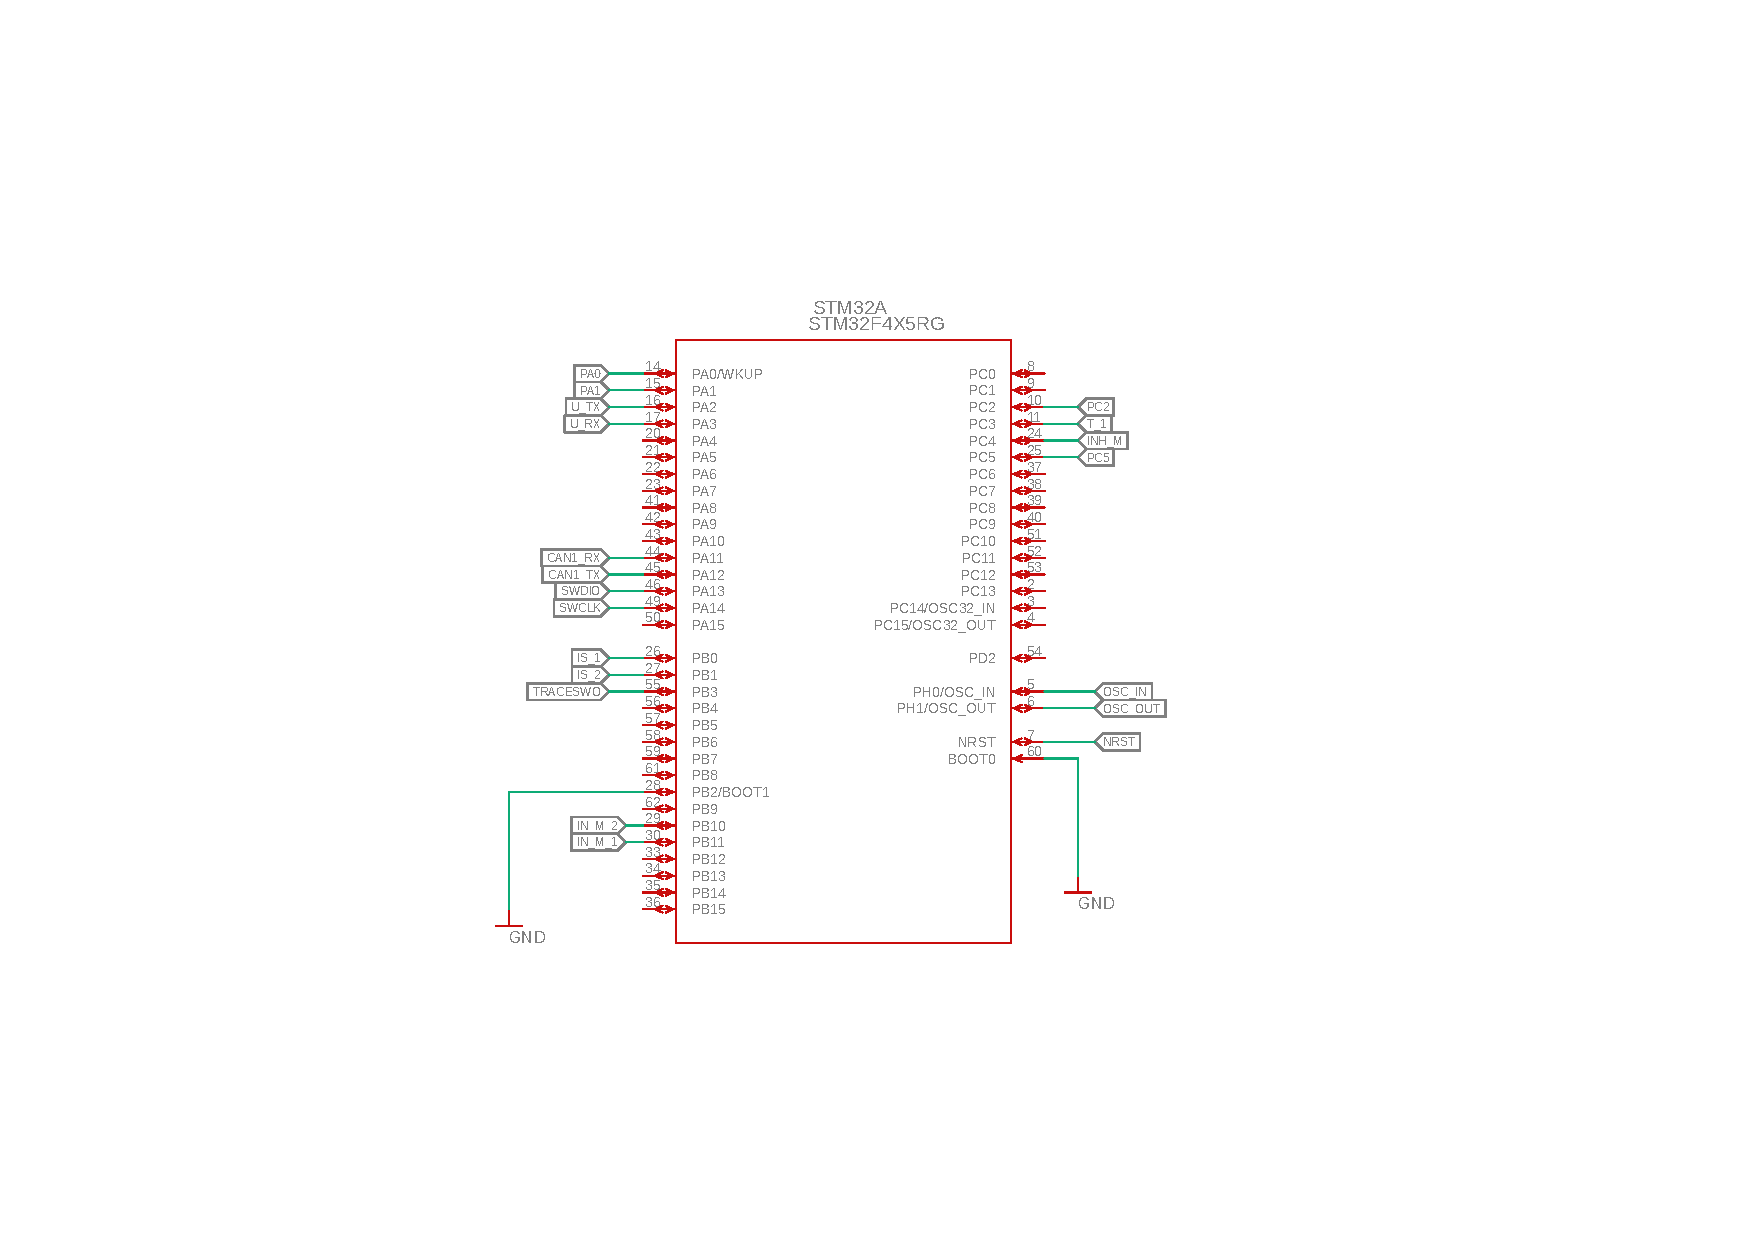
\includegraphics[width=\textwidth]{./Bilder/MCU_PINS.pdf}
\end{minipage}
\noindent\begin{minipage}{0.1\textwidth}
\begin{tabular}{l | l}
			Pin & Funktion\\ \hline
			PA0& Sensorik\\
			PA1& Sensorik\\
			PB0& Sensorik\\
			PB1& Sensorik\\
			PC2& Sensorik\\
			PC3& Sensorik\\
			PC5& Sensorik\\
			PA2& UART\\
			PA3& UART\\
			PA11& CAN\\
			PA12& CAN\\
			PA13&SWD\\
			PA14&SWD\\
			PB3& SWD\\
			PB0 & H-Brücke\\
			PB1 &H-Brücke\\
			PB10&H-Brücke\\
			PB11&H-Brücke\\
			PC4&H-Brücke\\
			OSC\_IN&Quarz\\
			OSC\_OUT&Quarz\\
			NRST & Reset
		\end{tabular}
\end{minipage}

\noindent\begin{minipage}{0.75\textwidth}
\captionof{figure}{Pin-Belegung des Mikrocontrollers}
\label{fig:mcupin}
\end{minipage}
\noindent\begin{minipage}{0.2\textwidth}
	\captionof{table}{Pin-outs}
	\label{tab:pins}
\end{minipage}
\hspace{1cm}
\newline
\\
Wichtig bei der Beschaltung ist außerdem die Belegung von BOOT0 und BOOT1, welche den Speicherbereich definieren aus dem der Mikrocontroller beim Startvorgang sein Programm lädt. Nach \autoref{tab:boot} muss für den Start im Main Flash memory BOOT0 auf GND-Niveau gesetzt werden, während die Belegung von BOOT1 undefiniert ist und somit mit GND belegt werden kann.

\begin{table}[H]%
\centering
\captionabove{Boot modes des STM32F405RGT7 nach \cite[S.69]{stmref}}
\begin{tabular}{c c c c}
BOOT1 & BOOT0 & Boot mode & Aliasing \\ \hline
x & 0 & Main Flash memory & Main Flash memory is selected as the boot space\\
0 & 1 & System memory & System memory is selected as the boot space\\
1 & 1 & Embedded SRAM & Embedded SRAM is selected as the boot space
\end{tabular}

\label{tab:boot}
\end{table}

Um möglichst akurate Taktraten zu haben und somit Schaltvorgänge und Sensorikdaten genau und reproduzierbar zu gestalten, wird, wie vom Hersteller des Mikrocontrollers empfohlen, ein externer Taktgeber benutzt \cite[S.218]{stmref}. Auf der Platine wird hierbei ein ABLS-8.000MHZ-K4T von Abracon genutzt, welcher eine Nennfrequenz von 8MHz hat. \autoref{fig:quarz} zeigt die letztendliche Verschaltung auf der Platine. Die Lastkapazitäten CQ1 und CQ2 von \SI{22}{pF} sind dabei nach dem Datenblatt des Herstellers gewählt. Die Widerstände R19 und R20 sind einerseits verbaut, um den externen Quarz vom Mikrocontroller trennen zu können, andererseits wird R20 benutzt, um den Stromfluss des Quarzes zu beschränken \cite[S.16]{stmquarz}. Nach \cite[S.16]{stmquarz} lässt sich eine Abschätzung von R20 über
\begin{align*}
R_{20} = \frac{1}{2\pi f C_{Q1}}
\end{align*}
gewinnen. Damit ergibt für R20 sich ein Richtwert von etwa \SI{900}{\Omega} bei CQ1 = 22pF. Ein zu niedriger Widerstand erhöht die Verlustleistung über den Quarz, während ein höherer Widerstand zum Stillstand der Oszillation führen kann. Auf der Platine ist ein Widerstand von \SI{1}{k\Omega} gewählt.

\begin{figure}[H]%
\centering
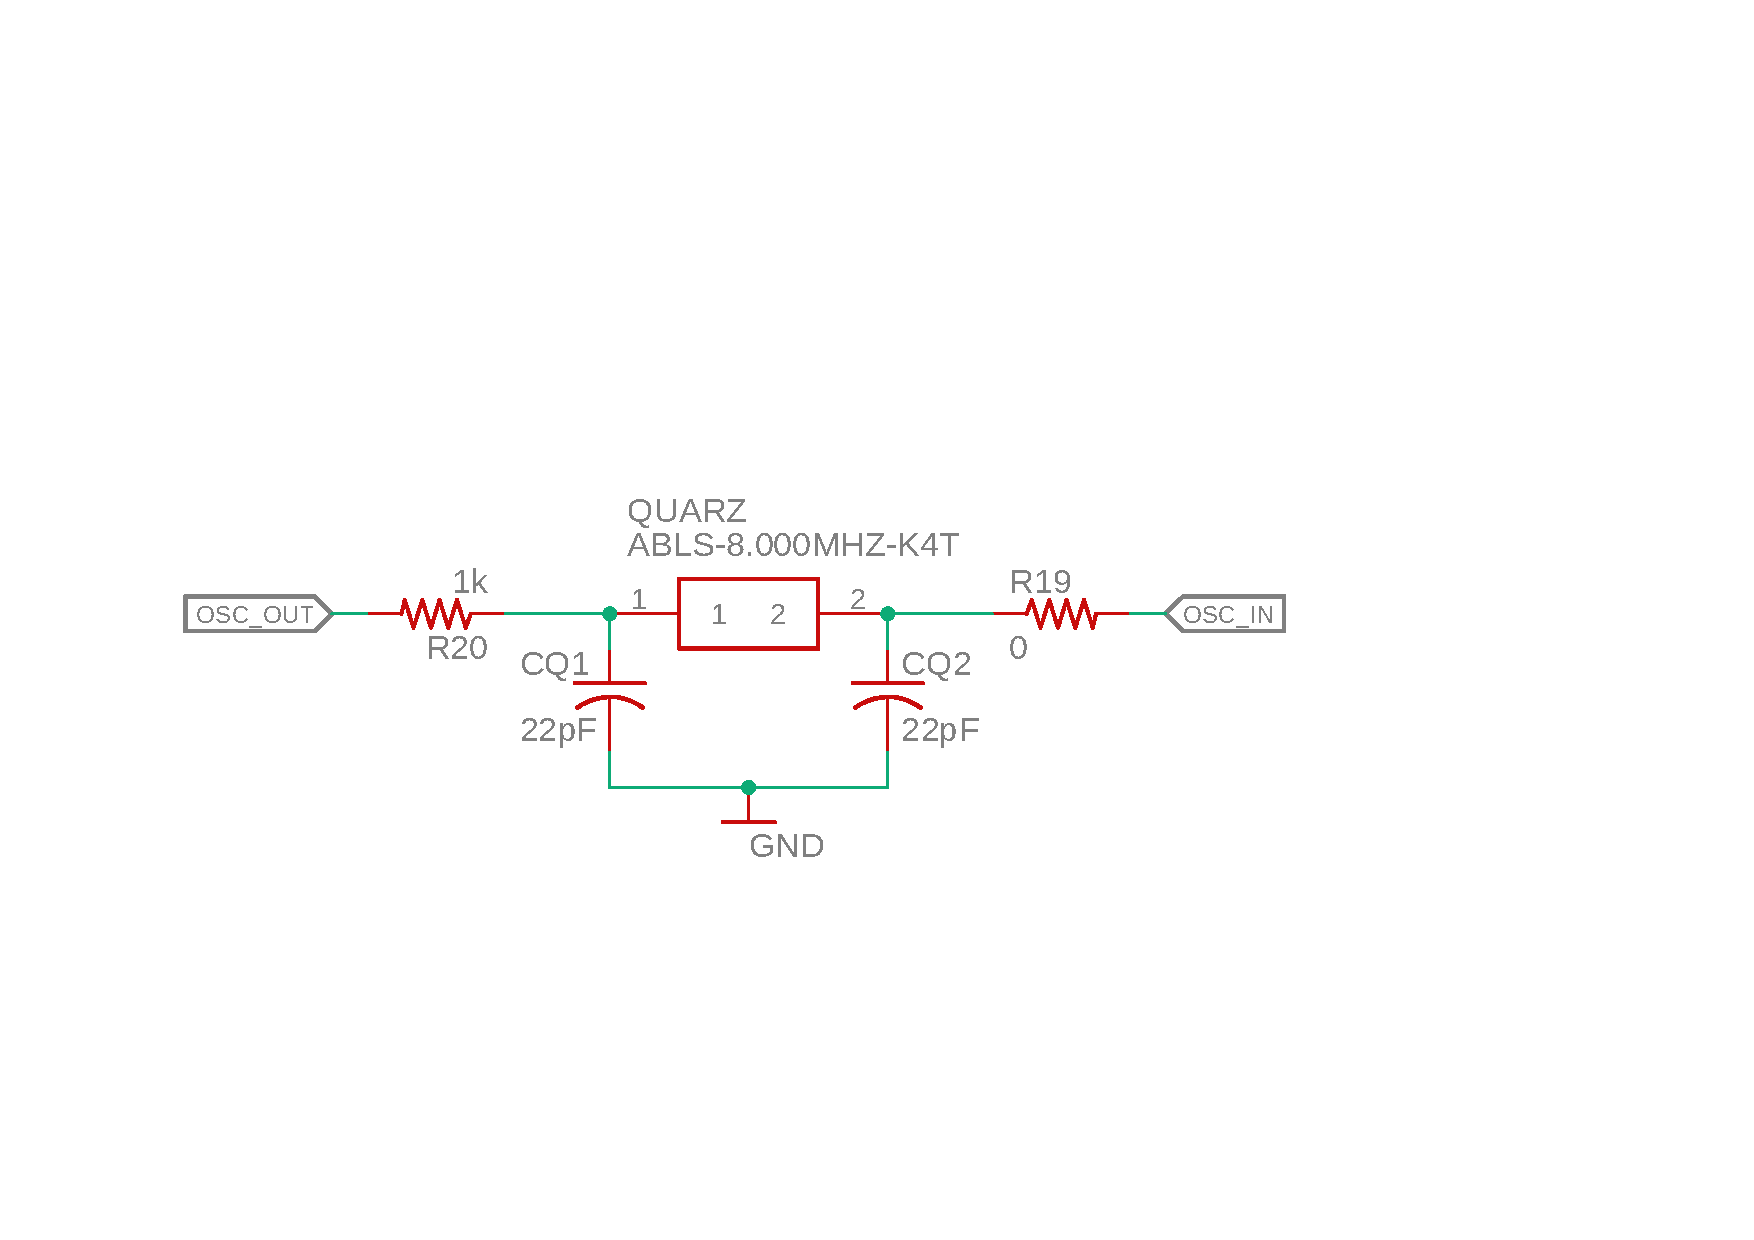
\includegraphics[width=300pt]{./Bilder/quarz.pdf}%
\caption{Anschluss externer Quarz}%
\label{fig:quarz}%
\end{figure}

\subsection{CAN-Transciever}
Zur Kommunikation des Mikrocontrollers mit der MicroAutobox ist eine Signalübertragung über CAN vorgesehen. Da der Mikrocontroller die physikalischen Bussignale nicht verarbeiten kann, wird die Kommunikation des Mikrocontrollers mit dem Bussystem über einen CAN-Transciever gestaltet. Dieser sorgt dafür, dass den Mikrocontroller nur für ihn lesbare Daten erreichen und übersetzt gleichzeitig die vom Mikrocontroller ins Bussystem gesendete Nachrichten. Die Pins des Mikrocontrollers für diese Aufgaben sind CAN1-RX zum Erhalten von Informationen und CAN1-TX zum Senden von CAN-Nachrichten. Auf Busebene gibt es die Signale CAN-HIGH und CAN-LOW, welche in \autoref{sec:CAN_KAP2} beschrieben wurden. In \autoref{fig:cantrans} ist die Verschaltung des CAN-Transcievers SNHVD230QD von Texas Instruments zu sehen. An Pin VCC wird die Spannungsversorgung von \SI{3,3}{V} angeschlossen. VREF ist ein Ausgangspin mit halber VCC-Spannung beispielsweise zum Entwerfen einer Split-Termination. Pin D ist der Anschlusspin für die gesendeten Nachrichten des Mikrocontrollers über CAN1-TX. Pin R sendet die übersetzten CAN-Nachrichten des Bussystems an CAN1-RX.
\begin{figure}[H]%
\centering
\includegraphics[width=400pt]{./Bilder/can.pdf}%
\caption{CAN-Transciever Verschaltung}%
\label{fig:cantrans}%
\end{figure}\noindent
Über den Pin RS lassen sich durch den Widerstand R\_RS verschiedene \textit{slew rates} einstellen und damit, wie schnell der Ausgangstransistor bei der Übermittlung von Nachrichten durchschaltet \cite[2]{cantrans}. Für einen Widerstandswert von \SI{0}{\Omega} ist die Geschwindigkeit maximal, während sie bei \SI{10}{k\Omega} etwa \SI{15}{\frac{V}{\mu s}} beträgt. Zwischen CAN-HIGH und CAN-LOW wird nach dem Datenblatt ein \SI{120}{\Omega} geschaltet. Bei der Wahl von R5 und R\_RS wurde sich an der bestehenden Konfiguration des STM-Discovery-Shields orientiert, mit der die CAN-Kommunikation aufgebaut wurde. 

\subsection{Spannungsversorgung}\label{sec:spannver}
Die Elektronik wird weiterhin mit dem bisher verwendeten Manson SBC-2130 Battery Charger versorgt. Dieser stellt eine konstante Spannung von \SI{13,8}{V}. Da die verschiedenen Komponenten jedoch Versorgungsspannungen von \SI{3,3}{V} und \SI{5}{V} benötigen, muss die Schaltung durch einen Spannungsregler erweitert werden. Zusätzlich werden dadurch Schwankungen in der Eingangsspannung geglättet. 

\subsubsection{Low Dropout Spannungsregler}
Ein LDO ist ein Festspannungsregler, der eine festgelegte und somit invariable Ausgangsspannung liefert, die sich auch dann nicht ändert, wenn die Eingangsspannung schwankt. Die Schaltung eines LDO-Reglers besteht aus einer Referenzspannungsquelle, einem Differenzverstärker und einem Stellglied in Form eines Leistungstransistors. Die hier verwendeten Ausführungen sind P-Kanal-MOSFET-basierte Regler. Das Blockschaltbild eines solchen LDOs ist in folgender Abbildung schematisch dargestellt.\\
\begin{figure}[H]
	\centering
		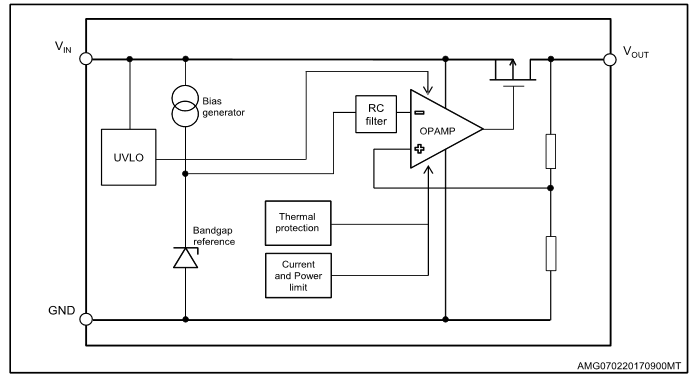
\includegraphics[width=350pt]{./Bilder/LDO.png}
	\caption{Blockschaltbild LDO nach \cite{ldo}}
	\label{fig:LDO2}
\end{figure} \noindent
Der Differenzverstärker vergleicht die Ausgangsspannung mit einer stabilen Referenzquelle aus einer Zenerdiode, sodass die gemessene Spannungsabweichung über das Stellglied ausgeregelt werden kann. Ist die Ausgangsspannung zu niedrig, so wird der Transistor stärker angesteuert bis die geforderte Ausgangsspannung erreicht wird. Im umgekehrten Fall wird der Strom über den Transistor reduziert. Der Transistor wird in dieser Schaltung wie ein veränderlicher Widerstand verwendet, an dem die überflüssige Spannungsdifferenz abfällt und in Wärme umgewandelt wird. Die verwendeten LDOs besitzen außerdem eine Strombegrenzungsschaltung und eine Schutzschaltung, die die Betriebstemperatur überwacht und das Bauteil vor thermischer Überlastung schützt, sowie eine Unterspannungsabschaltung. 

\subsubsection{Verschaltung auf Platine}
Grund für die Wahl dieser Art von Spannungsreglern für die Platine ist ihre kompakte Bauform, ihr günstiger Einkaufspreis und das geringe Rauschen im Vergleich zu Schaltreglern, da keine Schaltvorgänge auftreten. Auf der Platine werden LDOs vom Typ LDL1117 von STMicroelectronics verwendet. Für die \SI{3,3}{V} Versorgung ist dies der LDL1117S33R und für die \SI{5}{V} der LDL1117S50R LDO. Nach dem Datenblatt \cite[S.7]{ldo} ist die Eingangskapazität zu \SI{1}{\mu F} und die Ausgangskapazität zu \SI{4,7}{\mu F} zu wählen. Diese werden aus Stabilitätsgründen und zur Entkopplung verwendet. Empfohlen wird weiterhin Keramikkondensatoren zu verwenden, welche X5R oder X7R Dielektrika aufweisen. In \autoref{fig:volt} ist der Schaltplan der Spannungsversorgung für die Platine zu sehen. An VIN wird die Batteriespannung angelegt, welche mit \SI{1}{\mu F} gegen GND entkoppelt wird. An VOUT liegen die jeweiligen \SI{3,3}{V} bzw. \SI{5}{V} an, welche jeweils über \SI{4,7}{\mu F} gegen GND geschaltet sind. Zur allgemeinen Spannungsglättung wird eine Kapazität C13 von \SI{1000}{\mu F} zwischen der Batteriespannung und GND geschaltet, welche starke Schwankungen beim Durchschalten der H-Brücke verhindern soll.

\begin{figure}[H]%
\centering
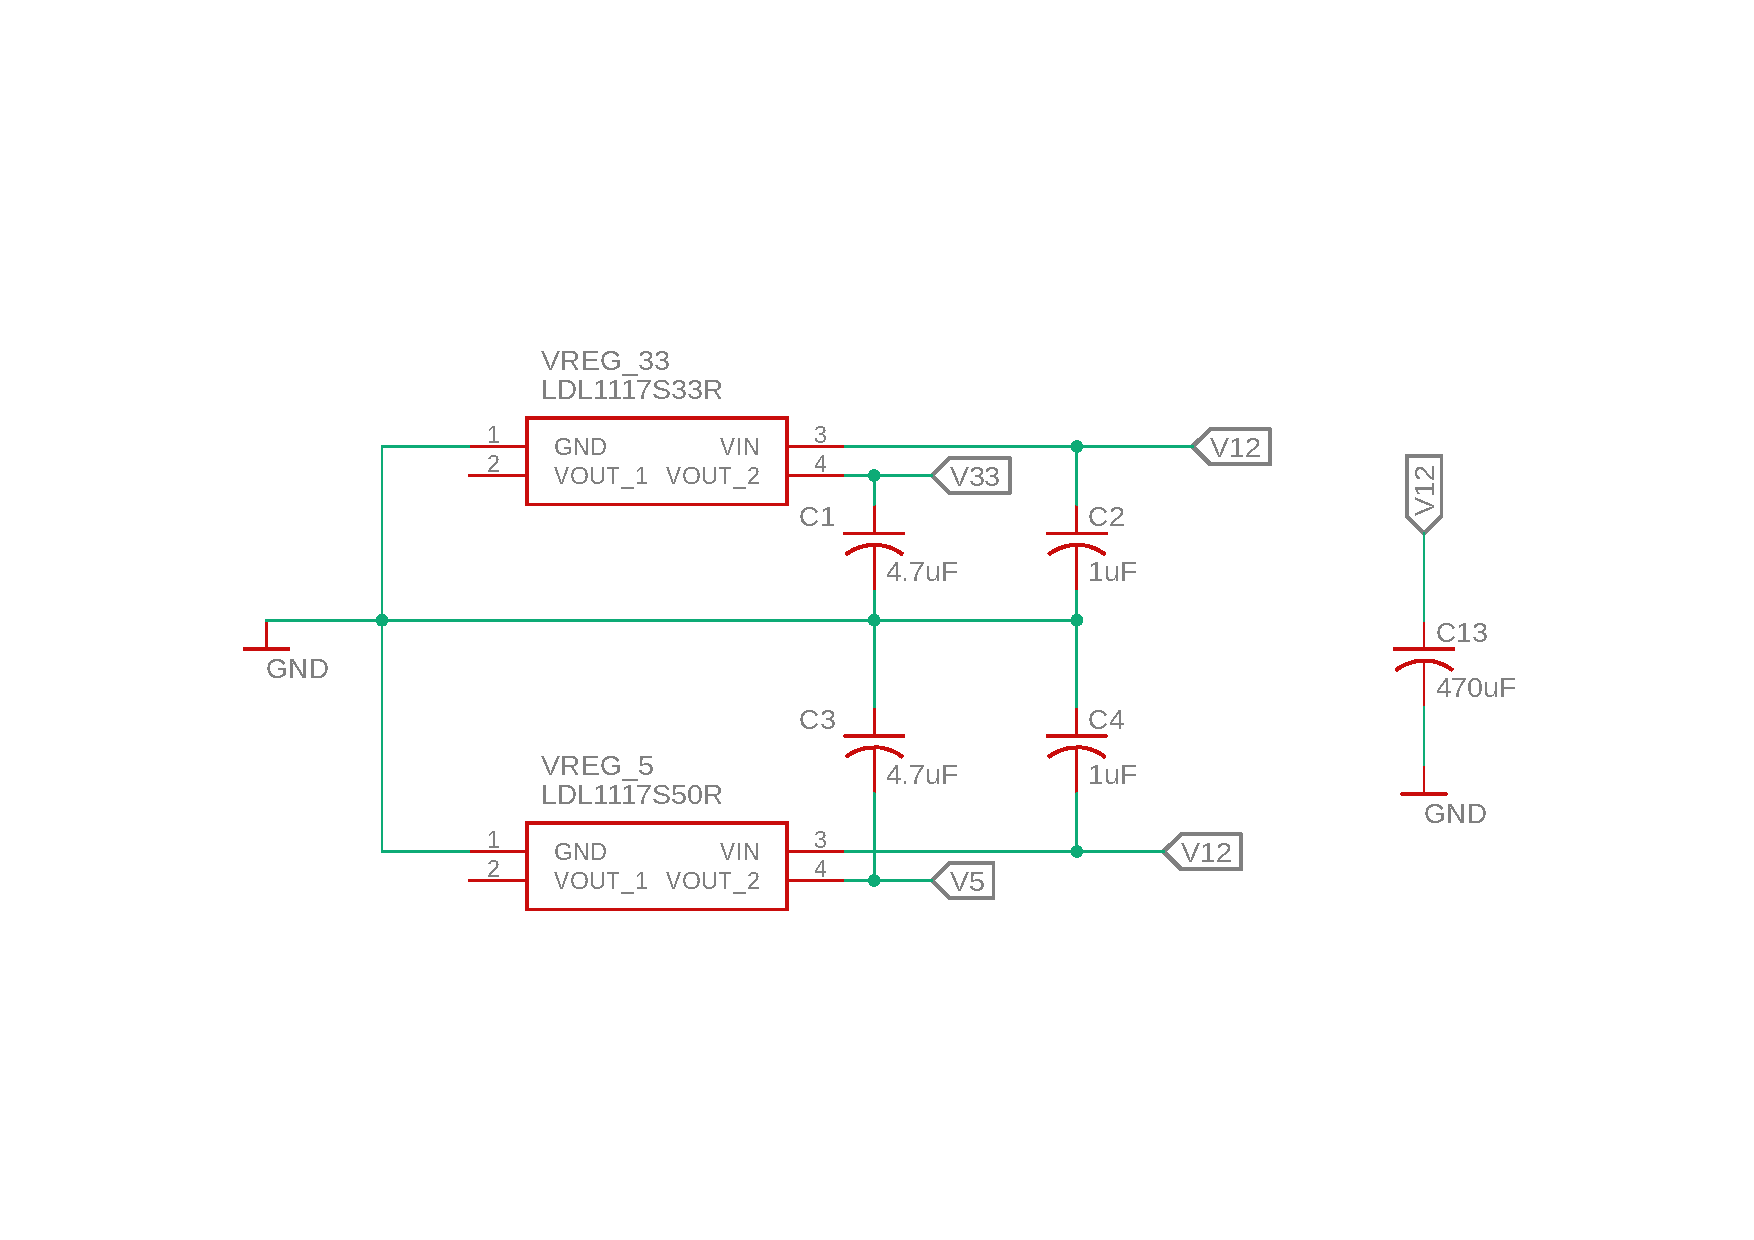
\includegraphics[width=410pt]{./Bilder/volt.pdf}%
\caption{Schaltplan Spannungsversorgung}%
\label{fig:volt}%
\end{figure}

\section{Platinenanschluss}\label{sec:stecker}
Die Platine wird mit einem 1-776267-1 Stecker von TE Connectivity verbunden, um notwendige Signalleitungen nach Außen zu führen und zusätzlich Spannungsversorgung und Lagesensorik mit der Platine verbinden zu können. In \autoref{fig:stecker} ist die Pin-Belegung des Steckers zu sehen. Um den Mikrocontroller über SWD programmieren zu können, muss der Stecker die notwendigen Signalleitungen SWDIO, SWCLK, TRACESWO, V33 und GND nach Außen führen. Diese werden direkt mit einem ST-Link/V2 nach \autoref{app:stlink} verbunden, sodass Programme von einem Computer auf den Mikrocontroller übertragen werden können. Zusätzlich muss der Mikrocontroller zur Programmierung mit Spannung versorgt werden, sodass der Stecker mit der Autobatterie verbunden sein muss. Weiterhin soll der Mikrocontroller über CAN-Signale mit der MicroAutobox kommunizieren können. Dazu werden die Schnittstellen CANH (CAN-HIGH) und CANL (CAN-LOW) über den Stecker nach außen geführt. Die Steckerpins V5, L\_1, L\_2 und GND werden für die Lagesensorik benötigt. Pin 4 und Pin 5 sind beide mit der Batterie verbunden und bilden die Spannungsversorgung der gesamten Platine. Aufgrund der potentiell hohen Ströme wird die Versorgung über zwei Pins zugeführt. Über den NRST-Pin lässt sich der Mikrocontroller zurücksetzen.\\ Als Gegenstück des Steckers existieren drei verschiedene Varianten. Jeweils eine Variante sind Programmier- und Betriebsstecker, die dritte Variante vereint diese beiden Optionen. Der Programmierstecker beinhaltet dabei alle Eingänge der oben genannten Signalleitungen, die zum Flashen des Mikrocontrollers über SWD nötig sind, und wird nur kurzzeitig verwendet. Im Dauerbetrieb wird der Betriebsstecker verbunden, welcher die Leitungen zur Spannungsversorgung, Lagesensorik und CAN-Kommunikation führt. Der kombinierte Stecker ist vor allem in der Entwicklungsphase hilfreich, um nicht ständig den Anschluss wechseln zu müssen. 


\begin{figure}[H]%
\centering
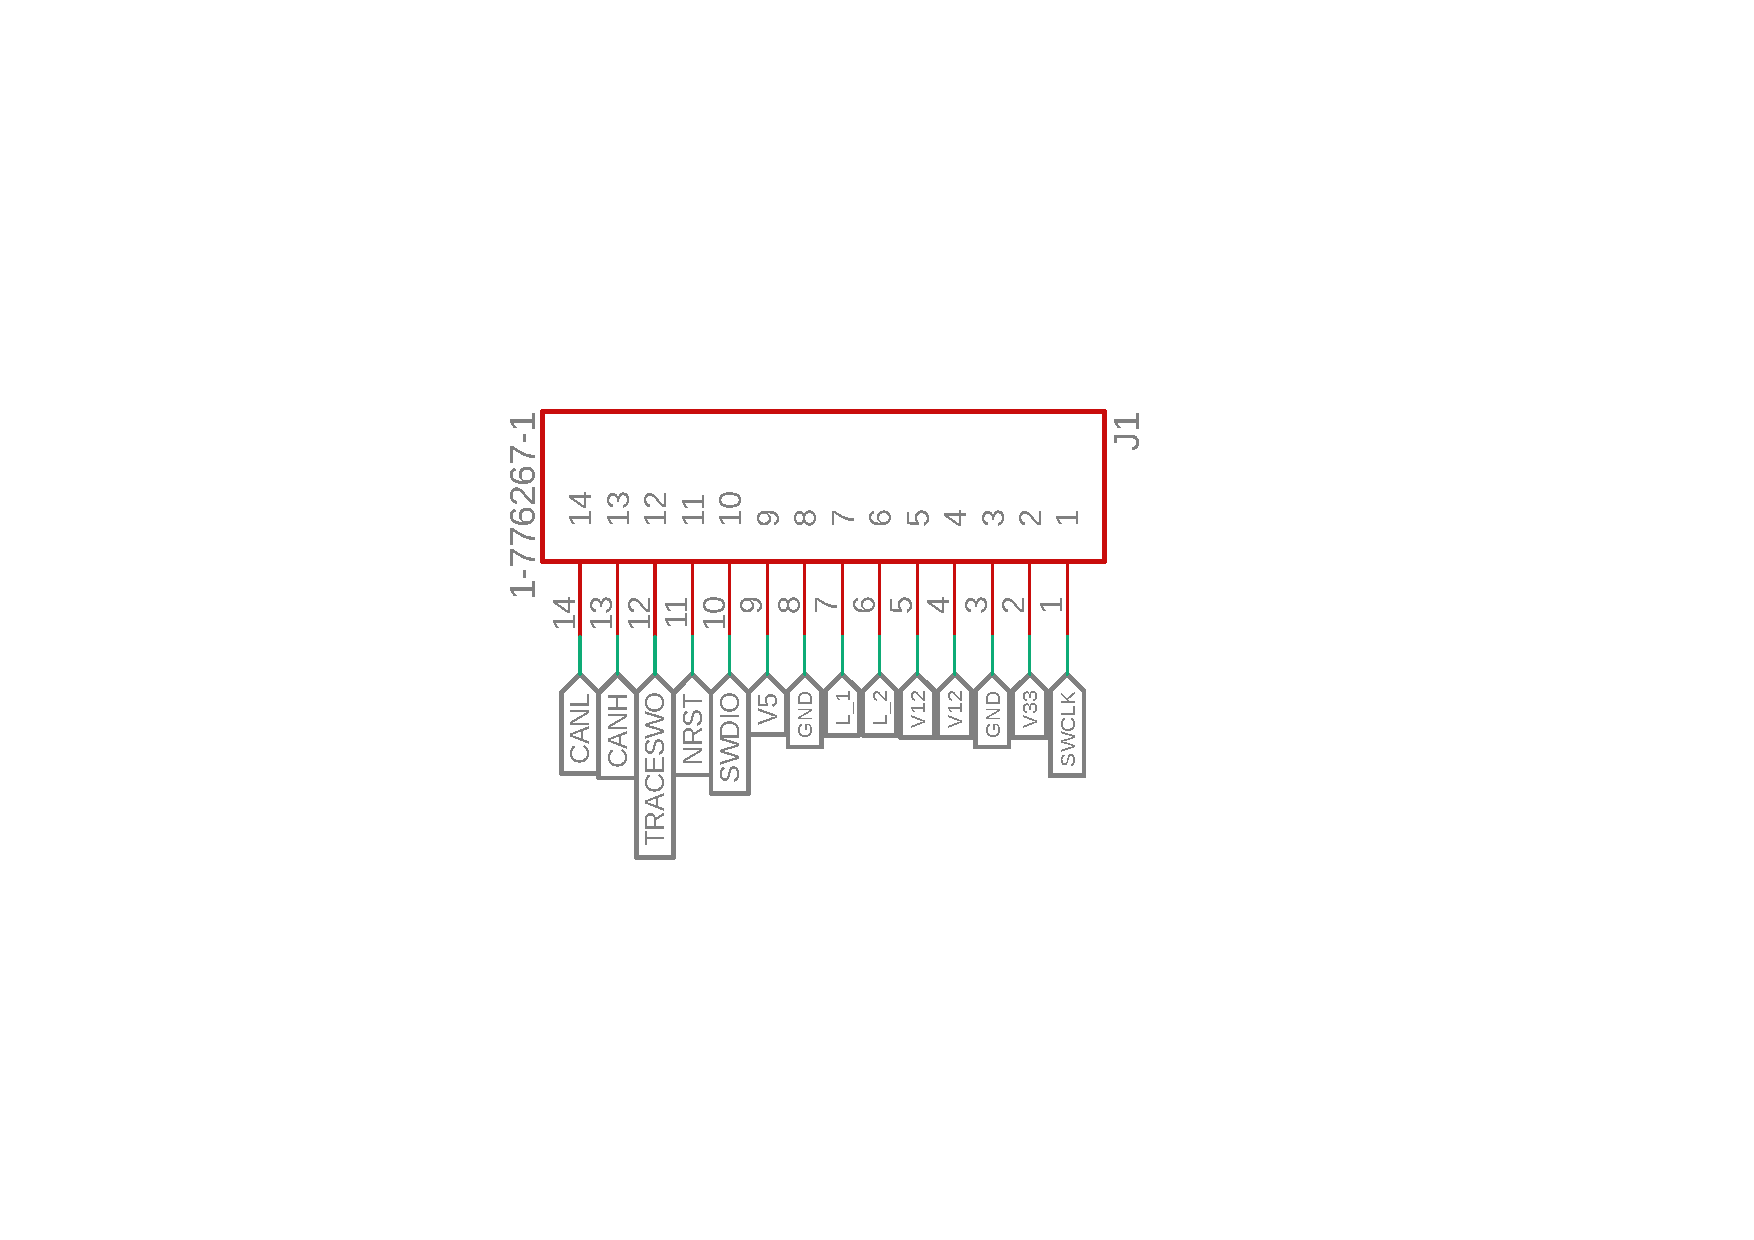
\includegraphics[width=200pt]{./Bilder/stecker.pdf}%
\caption{Anschlusspins Stecker}%
\label{fig:stecker}%
\end{figure}

\section{H-Brücke}\label{sec:hbridge}
Um den Aktor in beide Richtungen  betreiben zu können wird eine elektronische Schaltung benötigt, welche eine Stromrichtungsumkehr ermöglicht. Eine einfache Möglichkeit bietet die sogenannte H-Brückenschaltung, die vereinfacht in \autoref{fig:hbruecke} dargestellt ist. Eine H-Brücke ist eine Vollbrücke bestehend aus vier Schaltern und demnach ein Vierquadrantensteller. Werden die Schalter $S_1$ und $S_4$ geschlossen, kommt es zu einem Stromfluss durch den Aktor. Werden hingegen ausschließlich die Schalter $S_2$ und $S_3$ geschlossen, fließt der Strom entgegengesetzt. Ein Kurzschluss entsteht, wenn $S_1$ und $S_3$ oder $S_2$ und $S_4$ gleichzeitig geschlossen werden. Die Kombination aus Schließung von $S_1$ und $S_2$ oder $S_3$ und $S_4$ resultiert in einem offenen Schaltkreis. \\
\begin{figure} [H]
	\centering
	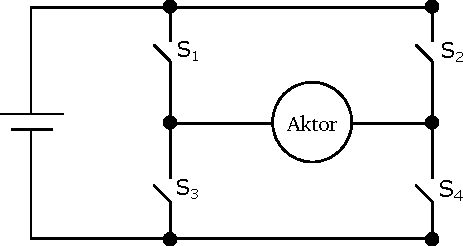
\includegraphics[width=0.3\linewidth]{Bilder/hbruecke.pdf}
	\caption{Vereinfachter Aufbau einer H-Brücke}
	\label{fig:hbruecke}
\end{figure}\noindent
In realen Systemen werden die Schalter durch Transistoren realisiert. Um Kurzschlüsse zu vermeiden, bietet sich die Schaltung einer H-Brücke über zwei Halbbrücken-ICs an. Jede Halbbrücke besteht dabei aus zwei Transistoren, wobei die integrierte Schaltung verhindert, dass beide gleichzeitige durchschalten. Bisher wurde am Aktorprüfstand eine gekaufte H-Brückenschaltung verwenden, die auf zwei \textit{BTS7960}-Halbbrücken der Firma Infineon basiert. Diese lieferte in vorangegangenen Arbeiten zufriedenstellende Leistungsergebnisse. Da sie jedoch  lediglich einen maximalen Stromfluss von \SI{43}{A} zulässt, die Schaltung aber in Zukunft auch für einem Aktor mit \SI{55}{A} benutzt werden soll, kann sie für die zu entwickelnde H-Brücke nicht verwendet werden. Eine Alternative ist die \textit{BTN8982}-Halbbrücke, welche auch von der Firma Infineon produziert wird und für einen maximalen Strom von \SI{55}{A} ausgelegt ist. Das Blockdiagramm dieser Halbbrücken ist in \autoref{fig:btn8982} dargestellt. \\
\begin{figure} [H]
	\centering
	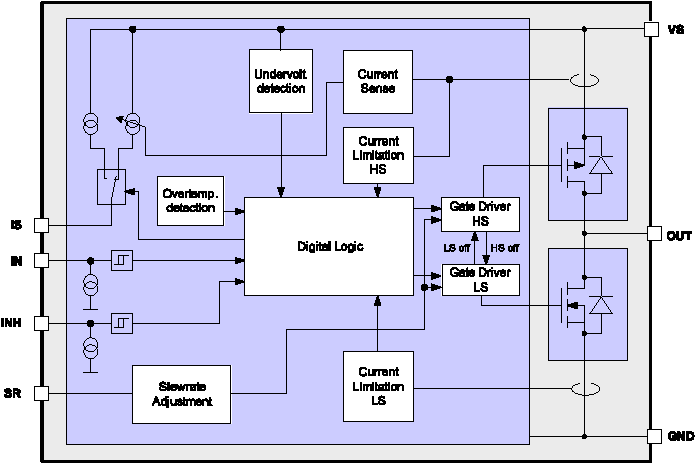
\includegraphics[width=0.5\linewidth]{Bilder/btn8982.pdf}
	\caption{Blockdiagramm der BTN8982 Halbbrücke \cite[S.4]{btn}}
	\label{fig:btn8982}
\end{figure}\noindent
Sie besteht aus einem \textit{p-channel highside MOSFET}, einem \textit{n-channel lowside MOSFET} und einem \textit{Driver IC}, die \textit{logic level inputs} unterstützt, wodurch der Anschluss an einen Microcontroller erleichtert wird. Die \textit{BTN8982} ist in einem Temperaturbereich von \SI{-40}{^\circ C} bis \SI{150}{^\circ C} einsetzbar und kann mit einer Versorgungsspannung von bis zu \SI{40}{V} betrieben werden, wobei diese im normalen Betrieb zwischen \SI{8}{V} bis \SI{18}{V} liegen sollte. Zusätzlich sind mehrere Schutzfunktionen integriert, beispielsweise ein Überstrom- und ein Übertemperaturschutz. Die \textit{BTN8982} besitzt acht Ausgänge, welche in \autoref{tab:Pinverteilung} aufgelistet und im Folgenden näher erläutert werden.

\begin{table}[H]
	\centering
		\captionabove{Pinverteilung Halbbrücken}
		\begin{tabular}{l p{2,5cm} p{8cm} p{3cm}}
			\textbf{Pin Nummer} & \textbf{Bezeichnung} & \textbf{Erläuterung} & \textbf{Anschluss an} \\ \hline
			1 & GND (Ground) & Erdung & Ground MCU \\
			2 & IN (Input) & definiert die Schalterstellung (1 = High Switch Mode; 0 = Low Switch Mode) & O-Pin MCU \\
			3 & INH (Inhibit) & 1: Betriebsmodus, 0: Schlafmodus & O-Pin MCU \\
			4, 8 & OUT (Output) & Ausgang der Brückenschaltung & Aktor \\
			5 & SR (Slew Rate) & Einstellen der Steigung der Spannungsantwort & Ground über Widerstand \\
			6 & IS (Status) & Strommessung \& Fehlererkennung & I-Pin MCU\\
			7 & VS (Supply) & Stromversorgung & Batterie\\
		\end{tabular}
	
	\label{tab:Pinverteilung}
\end{table}\noindent
Pin 1 ist der GND-Pin und bestimmt das Bezugsniveau der Versorgungsspannung, welche an Pin 7 angelegt wird. Ob Strom durch den highside MOSFET oder den lowside MOSFET fließt, wird durch Pin 2 (IN) bestimmt. Liegt eine 1 an fließt Strom durch den highside MOSFET, während bei einer 0 Strom durch letzteren fließt. Wird die Halbbrücke über ein PWM Signal geschaltet, geschieht dies über das Signal an diesem Pin. Der dritte Pin (INH) setzt die Halbbrücke in einen \textit{sleep-mode}, solange eine 0 anliegt. Somit kann die Halbbrücke nur genutzt werden, wenn eine 1 anliegt. Der \textit{sleep-mode} wird als Notaus verwendet, falls die Software einen kritischen Fehler detektiert (siehe \autoref{subsec:MOT}). Pin 4 und 8 (OUT) sind die Pins an die die Versorgungsspannung durchgeschaltet wird und stellen damit die direkte Schnittstelle mit dem Aktor da. Pin 5 (SR) bestimmt die Slew Rate des PWM Signals IN-Pin. Der sechste Pin (IS) ist für die Strommessung, sowie für die Meldung von Fehlern zuständig. Die Funktionsweise ist in \autoref{fig:IS_Pin} dargestellt.\\

\begin{figure} [H]
	\centering
	\includegraphics[width=0.7\linewidth]{Bilder/IS_Pin.pdf}
	\caption{Funktionsweise des IS \cite[S.18]{btn}}
	\label{fig:IS_Pin}
\end{figure}\noindent
Im normalen Operationsmodus (Current Sense Mode) liefert eine integrierte Stromquelle einen Strom $I_{is}$ der proportional zum durchgeschalteten Strom $I_{l}$ ist. Tritt ein Fehler auf wie zum Beispiel Übertemperatur oder Überstrom, schaltet die Halbbrücke in den Error Flag Mode. Hierbei wird die Stromquelle am IS-Pin gewechselt, welche einen konstanten Strom $I_{IS}$ liefert.  Dieser beträgt maximal \SI{6,5}{mA}. Der Proportionalitätsfaktor $k$ ist durch

\begin{equation}
k = \frac{I_{L1}-I_{L2}}{I_{IS}(I_{L2})-I_{IS}(I_{L1})}
\end{equation}\noindent
definiert und beträgt laut Datenblatt typischerweise 19.500. Messungen haben gezeigt, dass $k$ in der geschalteten H-Brücke unterhalb dieses Wertes liegt, sodass er als obere Abschätzung des geflossenen Stroms verwendet werden kann.
Die Spannungen an IN- und INH-Pins und somit auch die Funktionalität der H-Brücke wird durch einen hochgeschwindigkeits Leitungsverstärker/Puffer (\textit{CD74HCT125}) bereitgestellt. Leitungsverstärker sind elektronische Verstärkerschaltungen, die eingesetzt werden, um die Qualität elektrischer Signale zu verbessern \cite{Conrads2014}. Der schematischer Schaltplan des verwendeten Leitungsverstärkers und die zugehörige Logiktabelle in \autoref{fig:buffer} dargestellt. Der \textit{CD74HCT125} besitzt vier unabhängige Wege, die getrennt voneinander aktiviert werden können. Diese Aktivierung geschieht hierbei über ein \textit{Low Level} Spannungssignal am nOE-Pin. Low Level bedeutet, dass die Spannung maximal \SI{1,35}{V} betragen darf. Aufgrund des Platinendesigns \autoref{kap5} lässt sich dies recht problemlos bewerkstelligen, was neben der Hitzebeständigkeit und Schnelligkeit das Hauptargument für diesen Leitungsverstärker ist. Ist ein Weg aktiviert, sorgt ein \textit{High Level} Spannungssignal am Eingang (nA) dafür, dass die Versorgungspannung (VCC) an den jeweiligen Ausgang (nY) durchgeschaltet wird. In der ausgeführten Schaltung wird am VCC-Pin des \textit{CD74HCT125} eine Spannung von \SI{5}{V} angelegt. Die ersten drei Wege sind direkt mit GND verbunden, wodurch eine dauerhafte Aktivierung realisiert wird. Die ersten beide Wege sorgen für die Spannung an den IN-Pins der Halbbrücke, während der dritte Weg die INH-Pins versorgt. Die Eingänge sind dabei mit dem Microcontroller und die Ausgänge mit den Pins der Halbbrücke verbunden. Somit wird das PWM-Signal des Microcontrollers, welches eine maximale Spannung von \SI{3,3}{V} besitzt, auf ein PWM-Signal mit einer maximalen Spannung von \SI{5}{V} angehoben.

\begin{figure}[H]
	\begin{center}
		\noindent\begin{minipage}[h!]{0.45\textwidth} %Beginn der ersten Minipage
			\centering
			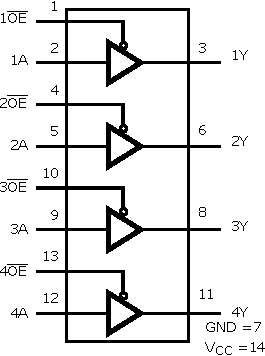
\includegraphics[height=0.85\textwidth]{Bilder/buffer.pdf}
		\end{minipage} %Ende der ersten Minipage
		\quad
		\begin{minipage}[h!]{0.45\textwidth} %Beginn der zweiten Minipage
			\centering
			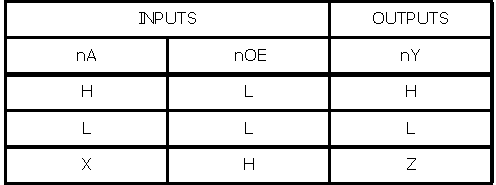
\includegraphics[height=0.3\textwidth]{Bilder/tabelle.pdf}
		\end{minipage} %Ende der zweiten Minipage
	\end{center}
	\caption{Schematischer Aufbau und Logiktabelle des CD74HCT125 Leitungsverstärkers}
	\label{fig:buffer}
\end{figure}\noindent
Die H-Brücke kann auch ohne einen Leitungsverstärker direkt mit dem Microcontroller verbunden werden, was zur Folge hätte, dass keine \SI{5}{V} sondern \SI{3,3}{V} Spannung an den Pins der H-Brücke anliegen. \autoref{fig:Strommessung} zeigt den geflossenen Strom durch den dabei angeschlossenen Aktor mit und ohne Leitungsverstärker bei variierenden PWM-Signalen. Es ist zu sehen, dass die Messung mit Geschalteten Leitungsverstärker deutlich symmetrischer sind, was auf eine bessere bidirektionale Schaltbarkeit schließen lässt. Außerdem sind die maximal durchgeschalteten Ströme größer. Dies lässt vermuten, dass die \SI{3,3}{V} nicht ausreichen um die Transistoren in den Halbbrücken vollständig schalten zu lassen. Dementsprechend wurde sich bei der endgültigen Schaltung für den Einsatz eines Leitungsverstärkers entschieden. 

\begin{figure} [H]
	\centering
	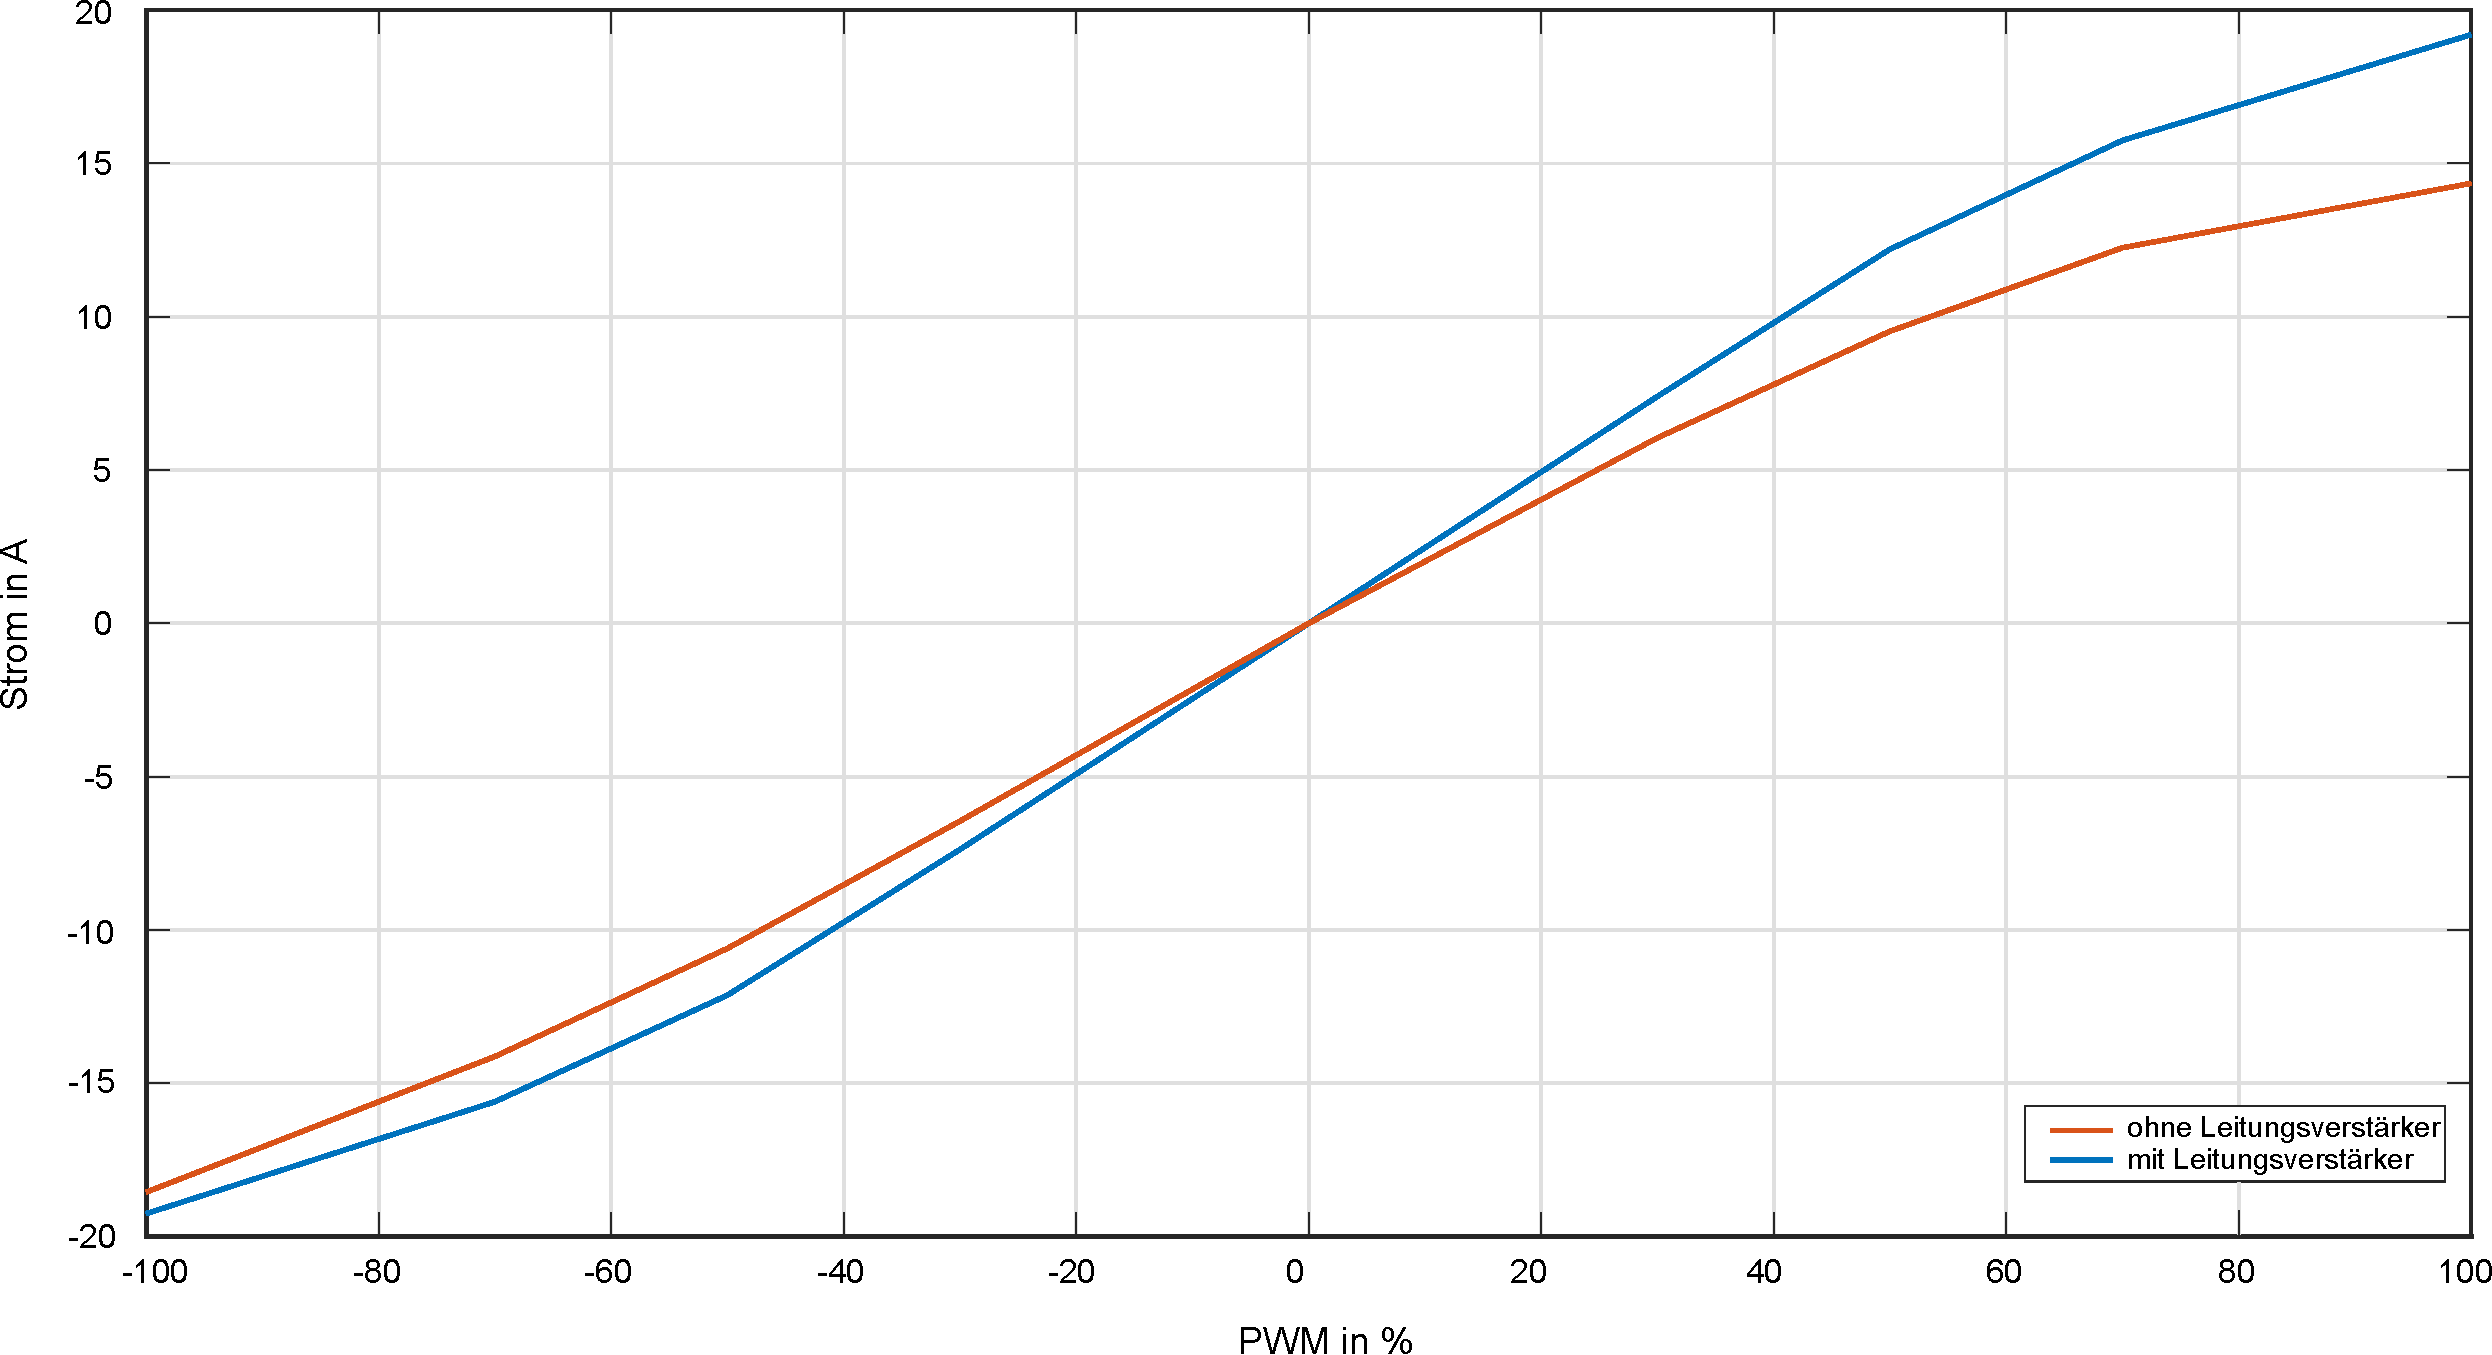
\includegraphics[width=0.8\linewidth]{Bilder/Strommessung.pdf}
	\caption{Strommessung mit und ohne Leitungsverstärker bei unterschiedlichen PWM-Signalen \cite[S.2]{Buffer}}
	\label{fig:Strommessung}
\end{figure}\noindent
Der schematische Aufbau der verwendeten H-Brücke ist in \autoref{fig:schematisch_hbruecke} zu sehen und wird im Folgenden genauer erläutert. Bei dem hier vorgestellten Aufbau wurde sich am Datenblatt der \textit{BTN8982}-Halbbrücken orientiert.

\begin{figure} [H]
	\centering
	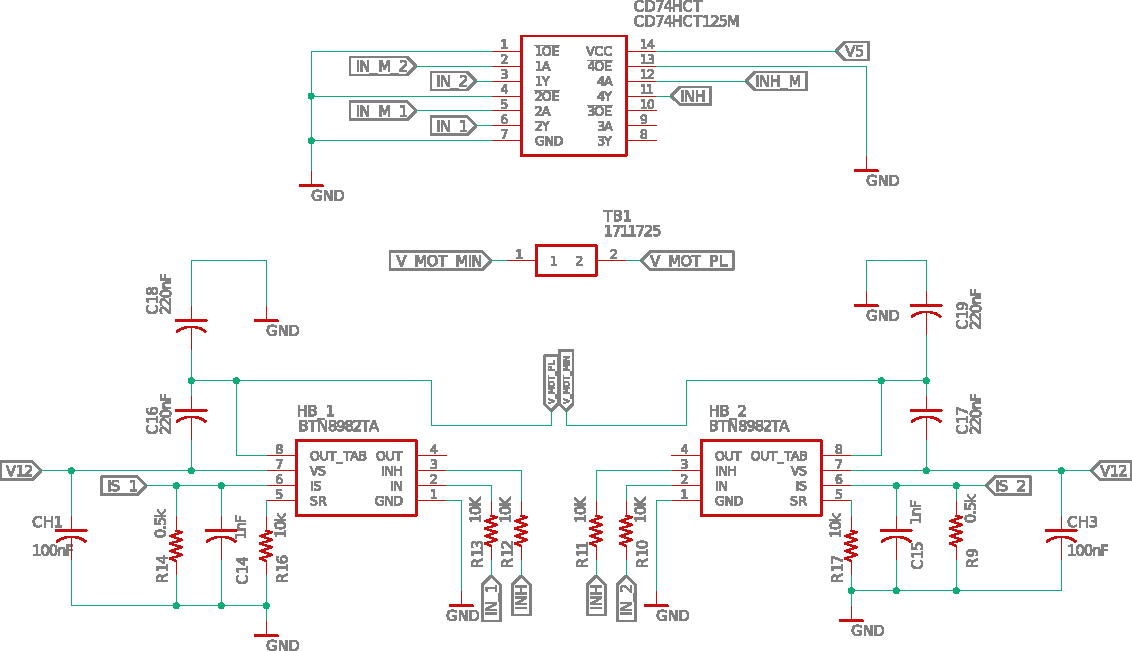
\includegraphics[width=1\linewidth]{Bilder/schematisch_hbruecke.pdf}
	\caption{Schematischer Aufbau der H-Brücke}
	\label{fig:schematisch_hbruecke}
\end{figure}\noindent
An beiden Halbbrücken wird am VS-Pin die Versorgungsspannung angelegt. Nahe am jeweiligen VS-Pin ist ein \SI{100}{nF} Kondensator (CH1, CH3) gegen GND geschaltet, welcher die Schwankungen der Versorgungsspannung, z.B. verursacht durch andere Komponenten, glättet. Ob diese Spannung an die OUT-Pins durchgeschaltet wird, hängt von der Spannung an den IN- und INH-Pins ab. Die INH-Pins setzen die Halbbrücken in einen \textit{sleep-mode}, wenn an ihnen keine Spannung zwischen 3 und \SI{5,3}{V} angelegt ist. Sofern diese Spannung anliegt, sorgt der gleiche Spannungsbereich am IN-Pin dafür, dass die Versorgungsspannung an die OUT-Pins der Halbbrücke durchgeschaltet wird. Jede Halb-Brücke besitzt zwei solcher OUT-Ausgänge, wobei einer über einen Pin und der andere über eine große Fläche auf der Rückseite realisiert wird. Letzterer eignet sich besser zum Übertragen großer Ströme, weshalb dieser zur Aktoransteuerung verwendet wird.  Die IN- und INH-Pins werden über \SI{10}{k\Omega} Widerstände (R10, R11, R12, R13) mit den Ausgängen des Leitungsverstärkers verbunden. Diese Widerstände werden zum Schutz der digitalen Eingänge benötigt.
Die IS-Pins der Halbbrücke werden direkt mit dem Mikrocontroller verbunden. Parallel sind \SI{0,5}{k\Omega} (R9, R14), sowie ein  \SI{1}{nF} Glättungskondensator (C14, C15) gegen GND geschaltet. Diese Pins sind für die Sensorik der Halbbrücke verantwortlich. An ihnen ist eine Stromquelle angeschlossen, die einen zum durchgeschalteten Strom proportionalen Strom liefert. Abhänging von den gegen GND geschalteten Widerständen ergibt sich eine Spannung die vom Mikrocontroller gemessen und aus der der durchgeschaltete Strom berechnet werden kann. Da der Strom am IS-Pin maximal \SI{6,5}{mA} beträgt, resultiert durch einen \SI{0,5}{k\Omega} eine maximale Spannung von \SI{3,25}{V} am Mikrocontroller. Ein größerer Widerstand hätte eine größere Spannung zur Folge, wodurch eine Schädigung des Mikrocontrollers nicht mehr ausgeschlossen werden kann. 
Die Widerstände, die zwischen SR-Pins und GND geschaltet sind (R16, R17), bestimmen die Slewrate des durchgeschalteten Signals. Dieser darf laut Datenblatt zwischen \SI{0}{\Omega} und \SI{51}{k\Omega} liegen. Der Hersteller bietet zudem eine Simulation an, in der verschiedene Slew-Rate-Widerstände getestet werden können. Die Ergebnisse einer solchen Simulation mit den eingestellten Widerständen \SI{0}{\Omega}, \SI{10}{k\Omega} und \SI{51}{k\Omega} sind anhand des durchgeschalteten Stroms $I_{OUT}$ in \autoref{fig:Simulationsergebnisse} dargestellt. Es ist zu sehen, dass der durchgeschaltete Strom mit zunehmendem Widerstand abnimmt, die Welligkeit jedoch nahezu gleich bleibt. Allerdings gilt es zu beachten, dass die \textit{Electromagnetical Interference} (kurz: EMI) für kleinere Slew-Rate-Widerstände ansteigt. Ein Widerstand von \SI{10}{k\Omega} stellt dabei einen guten Kompromiss dar und liefert auch in realen Messungen sehr gute Ergebnisse.
\begin{figure} [H]
	\centering
	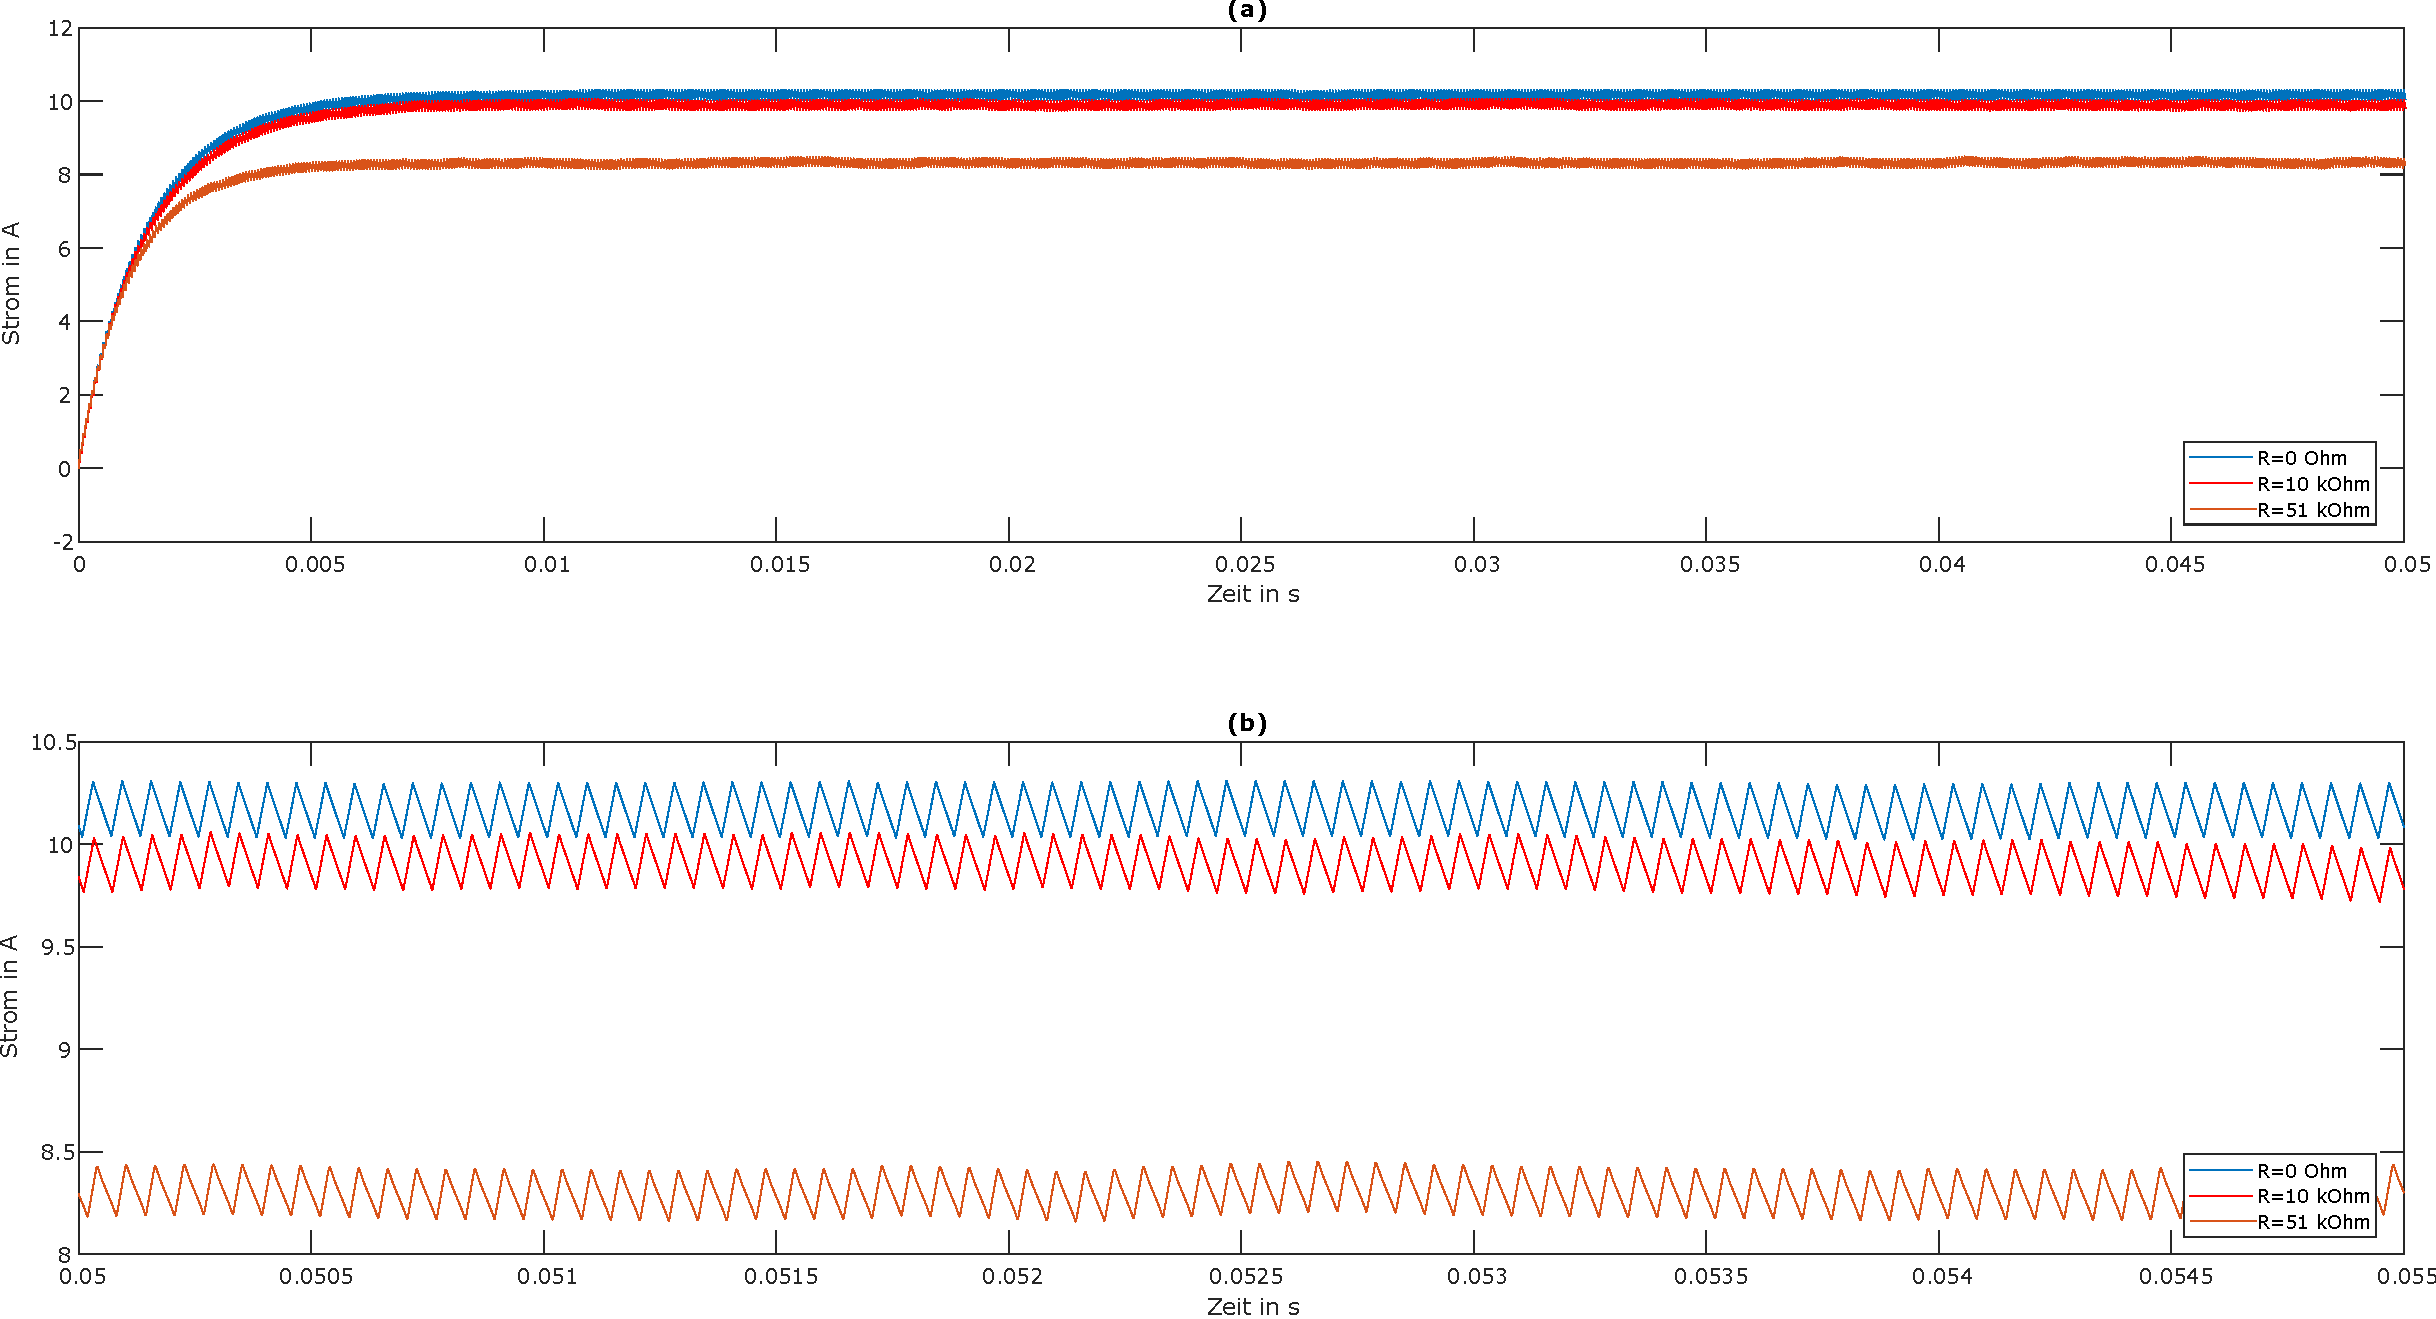
\includegraphics[width=1\linewidth]{Bilder/Simulationsergebnisse.pdf}
	\caption{(a):Simulationsergebnisse des durchgeschalteten Stroms über der Zeit aufgetragen; (b): Welligkeit des durchgeschalteten Stroms}
	\label{fig:Simulationsergebnisse}
\end{figure}\noindent
Bei der Simulation, sowie auch in der realen Anwendung, beträgt die Schaltfrequenz \SI{16}{kHz}. Dabei wurde sich an der vorangegangenen Arbeit orientiert, wobei auch höhere (\SI{20}{kHz}) und niedrige Frequenzen (\SI{10}{kHz}) getestet wurden. Höhere Schaltfrequenzen bieten prinzipiell den Vorteil, dass die Welligkeit des durchgeschalteten Stroms abnimmt. Allerdings steigt dabei auch die EMI. Der Unterschied der Welligkeit zwischen \SI{16}{kHz} und \SI{20}{kHz} ist jedoch vernachlässigbar klein, weshalb sich für die geringe EMI entschieden wurde. Im Gegensatz dazu ist bei \SI{10}{kHz} die Zunahme der Welligkeit deutlich zu beobachten.  

\section{Sensorik}
Die Sensorik des Gesamtsystems besteht aus einem Stromsensor, einem Temperatursensor und einem Lagesensor. Während die ersten beiden wichtige Kontroll- und Leistungsgrößen liefern, ist der Lagesensor essentiell für die Schaltvorgänge und damit die Funktionalität des Gesamtsystems. Der Stromsensor ist in den BTN8982 Halbbrücken integriert und ist bereits beschrieben. Die Funktionsweise und Verschaltung des Temperatur- und Lagesensors werden im folgenden erläutert. 

\subsection{Temperatursensor}\label{sub:temp}
Als Temperatursensor wird ein \textit{B57861S0103A039}-Thermistor verwendet. Dieser besteht aus einem Sensor und zwei \SI{350}{mm} langen Anschlusskabeln. Thermistoren sind elektrische Widerstände, deren Wert temperaturabhängig variiert. Dabei werden sie in die zwei Gruppen Heiß- und Kaltleiter aufgeteilt \cite{Stiny2015}. Da der \textit{B57861S0103A039}-Thermistor zur ersten Gruppe gehört, wird im folgenden ausschließlich auf diese eingegangen. Heißleiter besitzen einen negativen Temperaturkoeffizient (NTC), was bedeutet, dass ihr elektrische Widerstand sich mit steigender Temperatur reduziert. Dieser Zusammenhang ist allerdings hochgradig nichtlinear und kann durch 

\begin{equation} \label{eq:NTC}
R(T) = R_R \cdot e^{B\left(\frac{1}{T}-\frac{1}{T_R}\right)}  
\end{equation}
beschrieben werden mit der Referenztemperatur $T_R$, dem Widerstand $R_R$ bei der Referenztemperatur und dem Beta-Wert $B$. Als Referenztemperatur wird meistens \SI{25}{^\circ C} gewählt. Der Beta-Wert ist eine Materialkonstante, die üblicherweise zwischen \SI{1500}{K} und \SI{6000}{K} liegt \cite{Stiny2015}. Für den \textit{B57861S0103A039}-Thermistor beträgt der Widerstand $R_R$ \SI{10}{k\Omega} und der Beta-Wert $B$ \SI{3988}{K}. Der Betriebstemperatur liegt zwischen \SI{-55}{^\circ C} und \SI{155}{^\circ C}, was in den typischen Bereich für Heißleiter fällt \cite{Stiny2015}.\\
Eine mögliche Schaltung zur hochgenauen Temperaturmessung mittels Heißleitern ist die Wheatstonsche-Brückenschaltung (\autoref{fig:wheatstone}) bestehend aus drei ohmschen Widerständen und einem NTC-Thermistor \cite{Stiny2015}.

\begin{figure} [h]
	\centering
	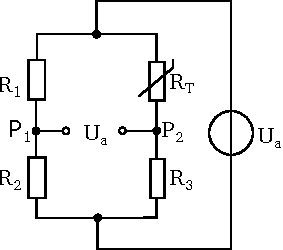
\includegraphics[width=0.4\linewidth]{Bilder/wheatstone.pdf}
	\caption{Wheatstone-Brückenschaltung}
	\label{fig:wheatstone}
\end{figure}\noindent
Solange die Brücke ausgeglichen ist, liegt keine Spannungsdifferenz zwischen $P_1$ und $P_4$ vor. Ändert sich der Widerstand des Thermistors, wird der ausgeglichene Zustand verlassen und es kommt zu einer Spannungsdifferenz, aus der der veränderte Widerstand des Thermistors bestimmt werden kann. Wird \autoref{eq:NTC} nach der Temperatur $T$ umgestellt, lässt sich daraus die aktuelle Temperatur berechnen. Aus Platzgründen auf der endgültigen Platine und da die hiermit erzielbare Genauigkeit nicht benötigt wird, ist stattdessen ein Spannungsteiler zum Einsatz gekommen. Dieser Spannungsteiler teilt den am Thermistor und an einem festen Widerstand abfallende Spannung und ist in \autoref{fig_ther_elek} dargestellt. Aus der Spannung, die am konstanten Widerstand $R_c$ abfällt, kann auf die Spannung geschlossen werden, die am Thermistor $R_t$ abfällt und somit auch auf dessen aktuellen Widerstand. Über \autoref{eq:NTC} ist dann ein direkter Zusammenhang zur gemessenen Temperatur gegeben.
Die Spannungsmessung findet im Mikrocontroller bzw. in dessen Analog-Digital-Convertern (ADC) statt. Dabei sind für eine möglichst exakte Messung mehrere Umstände zu beachten, die nun exemplarisch erörtert werden. Die Überlegungen gelten jedoch auch für die übrigen Spannungsteiler und ADCs. Im STM32F4 kommen \textit{successive approximation analog-to-digital converter} zum Einsatz, die eine Auflösung von bis zu \SI{12}{bit} liefern \cite{stmref}. Die Messdauer ist dabei konfigurierbar, entspricht jedoch mindestens für jedes Auflösungs-Bit und 3 zusätzliche Takte (12 + 3 Takte)\cite[S.397]{stmref}. Dieser Takt $f_{ADC}$ entspricht dabei nicht dem Kerntakt, sondern dem \textit{Advanced Peripheral Bus Clock} (APBC), der sich durch konfigurierbare Takt-Teiler vom Kerntakt unterscheidet. \\
Durch den Aufbau des ADC's bedingt, führen zu große Eingangswiderstände (bzw. Widerstandswerte im Spannungsteiler) zu großen Ungenauigkeiten. Dies ist umso kritischer je kürzer die Messdauer beträgt, da sich die interne Kapazität im ADC bei großen Eingangswiderständen nur langsam aufladen kann. Nach Ablauf der Abtastdauer sollte  jedoch die interne Kapazität auf die tatsächlichen Spannung am Eingangspin aufgeladen sein, sonst kommt es zu Abweichungen (siehe dazu auch \cite{ADC}, \cite{stm32}). ST stellt für den Mikrocontroller \autoref{eq:ADC} bereit, durch welche sich der maximale Eingangswiderstand 
\begin{equation} \label{eq:ADC}
R_{AIN} = \frac{(k-0,5)}{f_{ADC} C_{ADC} ln(2^{N+2})} - R_{ADC}
\end{equation}
abhängig der Messdauer berechnen lässt. Dabei entspricht $k$ den konfigurierten Messtakten pro Messung, $C_{ADC}$ der Kapazität des internen ADCs, $N$ der Auflösung und $R_{ADC}$ dem Schaltwiderstand des ADCs. Über $k$ und $f_{ADC}$ lässt sich dabei die Messdauer beeinflussen und somit die erlaubten Eingangswiderstände am Spannungsteiler beeinflussen. Für eine effektive Messdauer von \SI{2,7}{\mu s} muss der Eingangswiderstand unter \SI{31,355}{k\Omega} liegen, während bei einer Messdauer von nur \SI{1,5}{\mu s} nur Eingangswiderstände bis \SI{440,6}{\Omega} für hohe Genauigkeit zulässig sind. Der Nachteil niedrigere Widerstände im Spannungsteiler liegt jedoch in der Belastung des jeweiligen Sensorausgangs. Dort kann nur ein begrenzter Strom bereit gestellt werden. Daher bietet es sich an, eine Kapazität parallel zum Eingang des ADCs und somit zu $C_{ADC}$ zu schalten, die als Puffer für $C_{ADC}$ dient \cite{ADC}. Hier muss jedoch beachtet werden, dass eine weitere Kapazität zusätzlichen Bauraum, Kosten und Fehlerpotential zur Folge hat. Darüber hinaus werden schnelle Signaländerungen durch die RC-Zeitkonstante zum Auf-/Entladen des Kondensators ggf. herausgefiltert. Für den Thermistor werden keine kritischen Temperatursprünge erwartet, daher wird in diesem Fall eine zusätzliche Kapazität $C_c$ eingesetzt.\\
Auch durch einen Impedanzwandler, also eine Operationsverstärkerschaltung mit einer Spannungsverstärkung von $1$, lässt sich der Eingangswiderstand durch den Spannungsteiler kompensieren. Auch hier ergeben sich jedoch Nachteile durch benötigten Bauraum, anfallende Kosten, gesteigertes Fehlerpotential und zusätzliches Rauschen.\\
\begin{figure}[H]
	\centering
	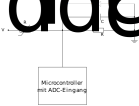
\includegraphics[width=0.5\linewidth]{./Bilder/fig_ther_elek}
	\caption{Schaltung zum Auslesen des Thermistors}
	\label{fig_ther_elek}
\end{figure}\noindent
Durch den Temperatursensor soll die Spulentemperatur im Tauchspulenaktor gemessen werden, da hier durch eine Überhitzung der Isolation Gefahrenpotential ausgeht. In der Umgebung der Spulen wird jedoch eine große Induktionswirkung erwartet, die die Genauigkeit der Spannungsmessung gefährden oder sogar ganz außerhalb des Messbereichs von \SI{0}{V} bis \SI{3,3}{V} liegen und somit die Funktionsfähigkeit des Mikrocontrollers gefährden \cite{stm32}. Eine Gegenmaßnahme stellt die Verseilung der Zuleiterkabel dar. Darüber hinaus kann durch die Schirmung der Kabel eine Schirmdämpfung erreicht werden, was die Induktionswirkung weiter reduziert \cite{Wolfsperger}. Falls trotzdem eine Spannung induziert wird, kann ein  Strom im mA-Bereich über interne Dioden im ADC abgeleitet werden \cite{stmref}. Um den Strom zu begrenzen, muss sich ein Widerstand zwischen induzierter Spannung und ADC-Eingang befinden. Eine weitere Methode den Pin vor einer Überspannung zu schützen, stellt eine Zener-Diode dar, die parallel zum Eingang des ADC's geschaltet wird (grau angedeutet). Hierbei ist jedoch darauf zu achten, dass auch im Normalbetrieb ein Kriechstrom durch die Diode fließt, der das Messergebnis verfälschen kann. \\
Um Probleme dieser Art zu umgehen, wurden auch alternative Sensorkonzepte in Betracht gezogen, die nicht über ein ADC ausgewertet werden. Diese haben sich jedoch als zu rechenaufwändig beim Auslesen erwiesen.

\subsection{Lagesensor}
Die Funktionsweise des PLCS-25M Sensors ist in \autoref{kap2} bereits erläutert worden. Der Sensor gibt demnach ein Spannungssignal aus, das nach \autoref{eq:Lage} in den Schaltgabelweg umgerechnet werden kann. Hierbei ist zu beachten, dass der Lagesensor mit \SI{5}{V} Gleichspannung betrieben wird und demnach der mögliche Ausgangsspannungsbereich zwischen \SI{0}{V} und \SI{5}{V} liegt, was außerhalb des gültigen Messbereichs der ADCs liegt. Über einen Spannungsteiler wird die Ausgangsspannung des Lagesensors demnach in den gültigen Messbereich übersetzt. Es gelten dabei bei der Auslegung des Spannungsteilers die gleichen Überlegungen wie in \autoref{sub:temp}. Um darüber hinaus eine Verbesserung der Positionsbestimmung zu erreichen, wird auch der komplementäre Ausgang des Lagesensors gemessen und entsprechend verrechnet. Der dadurch erreichte Genauigkeitsgewinn wird in \autoref{kap7} thematisiert.

\subsection{Sensorik Eingangsspannung}\label{eingangsspannung}
Um Fehlerzustände in der Spannungsversorgung feststellen zu können, ist ein einfacher Spannungsteiler zu entwerfen, anhand dessen die Eingangsspannung in einen für den ADC lesbaren Bereich gebracht wird. Es gelten die gleichen Überlegungen wie in \autoref{sub:temp}.


\chapter{Platinendesign}
\chapter{Software}\label{kap6}
Dieses Kapitel behandelt das zum Einsatz kommende Softwaresystem in Hinblick auf die verwendete Toolchain, die Programmstruktur als solche und Optimierungspotential. Dadurch soll dem Leser ein Überblick gegeben werden, sodass dieser den Programmablauf nachvollziehen kann und selbstständig Weiterentwicklungen durchführen kann.

\section{Toolchain}
Unter Toolchain werden die Werkzeuge bzw. Programme und ihr Zusammenwirken bezeichnet, die zur Programmentwicklung verwendet werden.\\ Für die vorliegende Aufgabenstellung ist ein Programm notwendig, das auf einem Mikrocontroller des Typs STM32F4 lauffähig ist. Zur Entwicklung des Programms kommt ein innovativer Ansatz zum Einsatz, der einfach verständlich und schnell erlernbar ist. Er basiert auf \textit{Matlab Simulink} und ermöglicht die Programmierung des Mikrocontrollers auf intuitive Weise. Um hardwarespezifische Blöcke bspw. zum Auslesen der ADCs nutzen zu können, wird ein Simulink Blockset namens \textit{Waijung} eingesetzt \cite{waijung}. Um das Blockschaltbild für den STM32 ausführbar zu machen, wird neben Simulink selbst auch der \textit{Simulink Coder} und der \textit{Embedded Coder} für Matlab benötigt. Durch diese Toolboxes ist es möglich aus einem Simulink Modell  C-Code zu generieren\cite{simulinkCoder}. Der \textit{Embedded Coder} führt dabei zusätzlich Optimierungen durch, die eine effiziente Ausführung auf einem eingebettetem System ermöglichen \cite{embeddedCoder}. 
Auch dieser C-Code ist nicht direkt ausführbar auf einem ARM-basierten Prozessor, wie es der STM32F4 ist. Es existieren jedoch geeignete Übersetzungstools (Compiler), die den C-Code in ARM-Assembler übersetzen und direkt lauffähig machen können. Im \textit{Waijung Blockset} werden dafür die \textit{GNU Tools for ARM embedded processors} mitgeliefert. Der kompilierte Code muss im letzten Schritt auf den Mikrocontroller übertragen werden, auch \textit{flashen} oder \textit{programmieren} genannt. Die Firma ST liefert dafür ein Programm namens \textit{STLink Utility}, welches neben des Programmiervorgangs über die definierte Programmierschnittstelle SWD auch Debugging-Fähigkeiten liefert, womit Fehlerzustände lokalisiert und beseitigt werden können. Einen groben Überblick über den Prozess vom Simulink  Modell bis zur Ausführung auf der Zielhardware wird in \autoref{fig_toolchain} gegeben.

\begin{figure}[H]%
\centering
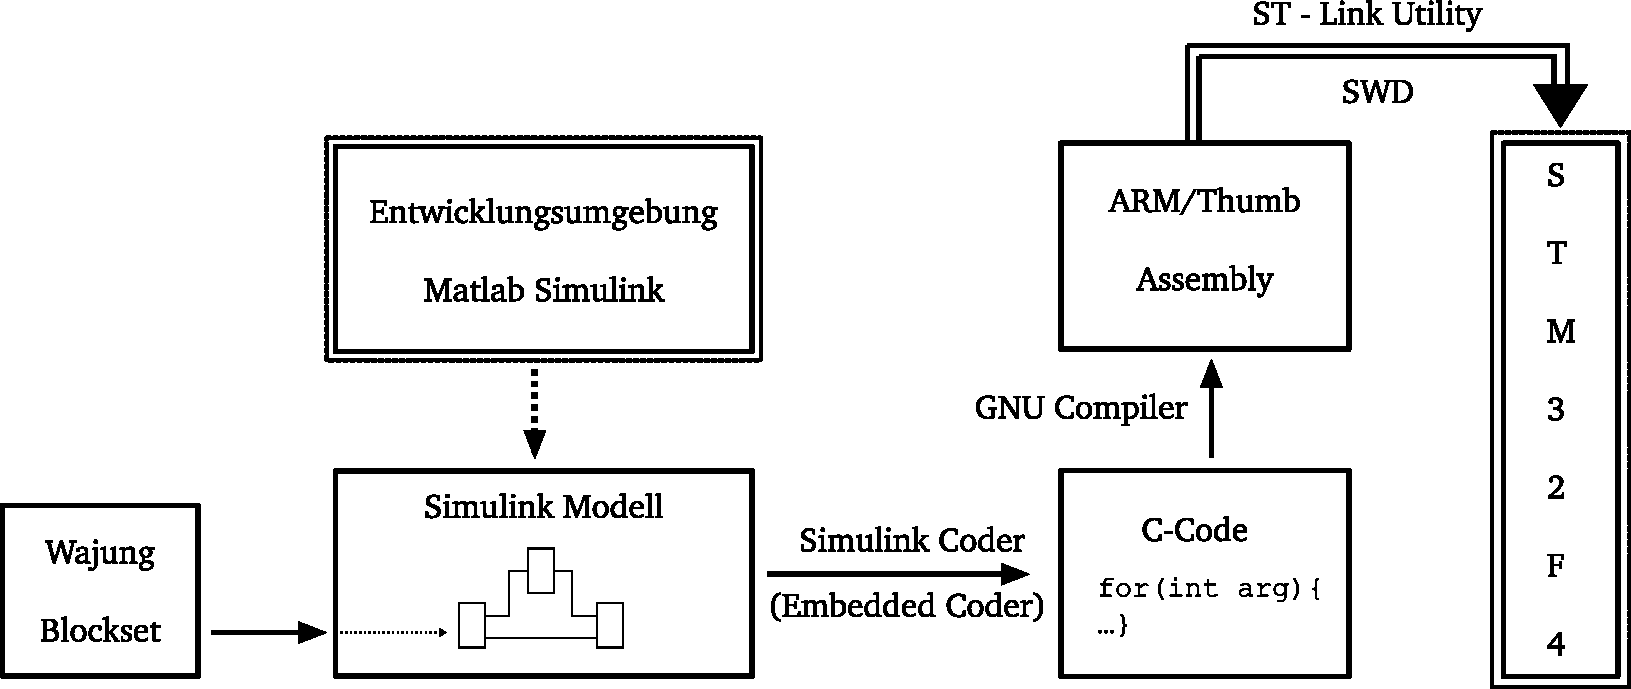
\includegraphics[width=0.8\columnwidth]{./Bilder/fig_toolchain}%
\caption{Vereinfachte Darstellung der eingesetzten Toolchain}%
\label{fig_toolchain}%
\end{figure}

\section{Vorstellung des Hauptprogramms}
Um einen Einblick in das Hauptprogramm zu bieten, das auf dem finalen Smart Actuator zum Einsatz kommt, wird zunächst geklärt welche Systemarchitektur zum Einsatz kommt.
Insbesondere im Gebiet des \textit{automated driving} sind viele Architekturansätze bekannt, durch welche komplexe Software strukturierter, robuster und zuverlässiger werden soll \cite{automated}.\\
 Weit verbreitet ist die 1983 entwickelte Architektur von Rasmussen, die zwischen wissensbasiertem, regelbasiertem und reflexbasiertem Verhalten unterscheidet. Unter reflexbasiertem Verhalten werden Aktionen verstanden, die rein reaktiv Sensordaten in Aktor-Aktivitäten umsetzen, ohne dabei komplexen Regeln zu folgen. Regelbasiertes Verhalten auf der anderen Seite ist bestimmt durch feste vordefinierte Regeln, die auf bestimmte Situationen angewendet werden. Falls eine Situation jedoch nicht vorhersehbar ist bzw. keine Regeln dafür hinterlegt sind, muss durch wissensbasiertes Verhalten gehandelt werden . Dieses Verhalten kann beispielsweise durch neuronale Netze erreicht werden, die jedoch in dieser Arbeit keine Anwendung finden. \cite{Rasmussen}\\
Wichtig sind daher die unteren beiden Ebenen, wobei nur die reflexbasierte Ebene Zugriff auf Sensorik und Aktorik hat. Auf übergeordneter regelbasierter Ebene werden dann vorverarbeitete Werte ausgewertet und anhand fester Regeln Handlungsanweisungen an die untere Ebene erzeugt. In \autoref{fig_arch} ist die Architektur nochmal vereinfacht dargestellt.
\begin{figure}[H]%
\centering
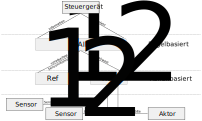
\includegraphics[width=0.8\columnwidth]{./Bilder/fig_arch}%
\caption{Drei-Ebenenarchitektur nach Rasmussen (vereinfacht)}%
\label{fig_arch}%
\end{figure}
Eine regelbasierte Hauptkomponente (MAIN) entscheidet je nach anliegenden vorverarbeiteten Sensorinformationen und Steuerbefehlen des übergeordneten Steuergeräts, welches Verhalten auf Reflexebene erwünscht ist. Es wird beispielsweise eine Sollgröße für einen Regler ($Ref_{2}$) vorgegeben, die schnellstmöglich ausgeregelt wird. \\
Konkret wird die Hauptkomponente durch einen Zustandsautomaten realisiert, der mehrere Ein- und Ausgänge zu anderen Komponenten bietet. Die Außendarstellung ist in \autoref{fig_main} dargestellt. Dabei sind links Eingänge von Sensorik- und CAN-Komponenten angeordnet und rechts Ausgänge. Die erste Buchstabenfolge beschreibt dabei jeweils von welchem Block das Signal ursprünglich generiert wird. Die Abkürzungen sind in \autoref{tab_kurz} erläutert. \\
Ein Vorteil dieser Architektur ist zunächst die Übersichtlichkeit und Nachvollziehbarkeit, da der gesamte Programmablauf in der Hauptkomponente nachvollzogen werden kann. Wie genau nämlich die Anweisungen dieser Hauptkomponente umgesetzt werden, ist für das Verständnis irrelevant. Darüber hinaus ist der wichtigste Vorteil, dass durch die strikte Trennung zwischen regelbasierter und reflexbasierter Ebene unterschiedliche Arbeitsfrequenzen realisiert werden können. Die aufwändige regelbasierte Ebene arbeitet dabei in der Regel langsamer. Weiterhin gelten die allgemeinen Vorteile beim Einsatz einer definierten Architektur wie Robustheit, Zuverlässigkeit, Wartbarkeit. Als Nachteilig ist anzusehen, dass sich der Entwickler durch die Anwendung dieser Architektur einschränkt und daher ggf. nicht zum idealen Ergebnis kommt. \cite{Rasmussen} \\
Eine klassische alternative Struktur stellt die \textit{Real-Time Control System Architecture} nach \cite{albus} dar. Diese besitzt ein breites Anwendungsspektrum, ist jedoch durch eine größere Anzahl an Ebenen komplexer und wird vornehmlich für intelligente Regelungen in unbekanntem Umfeld eingesetzt. \cite{albus}
\begin{table}%
\centering
\begin{tabular}{c c}
\hline
Abkürzung & Erläuterung \\
\hline
POS & Schaltgabelpositionsermittlung\\
CAN\_RECEIVE & empfangsseitge CAN-Schnittstelle \\
CAN\_TRANSMIT & sendeseitige CAN-Schnittstelle \\
CAL & Kalibrierung des Lagesensors\\
ERR & Fehlererkennung\\
MAIN & Hauptzustandsautomat\\
SEN & Sensorik\\
CONS & Regler zum Schalten\\
CONH & Regler zum Positionshalten\\
PWMS & Auswahlglied für PWM-Signal\\
MOT & Motortreiber \\

\end{tabular}
\caption{Erläuterung der Abkürzungen im Softwaresystem}
\label{tab_kurz}
\end{table} 

\subsection{Gesamtsystem}
In \autoref{fig_gesamtsystem} ist das gesamte Softwaresystem dargestellt. Hierbei ist die Sensorik hellblau, die Regelung hellgrün, die Aktorik dunkelgrün, die CAN-Kommunikation gelb und die Fehlererkennung orange dargestellt. Alle Komponenten agieren reflexbasiert direkt auf die Steuerungssignale des mittig angeordneten Hauptzustandsautomaten. Eine Ausnahme bildet die Kalibrierung, die ihrerseits durch einen Zustandsautomaten realisiert ist, wobei dieser durch den Hauptzustandsautomaten aktiviert und gestoppt wird. 
\begin{figure}[H]%
\centering
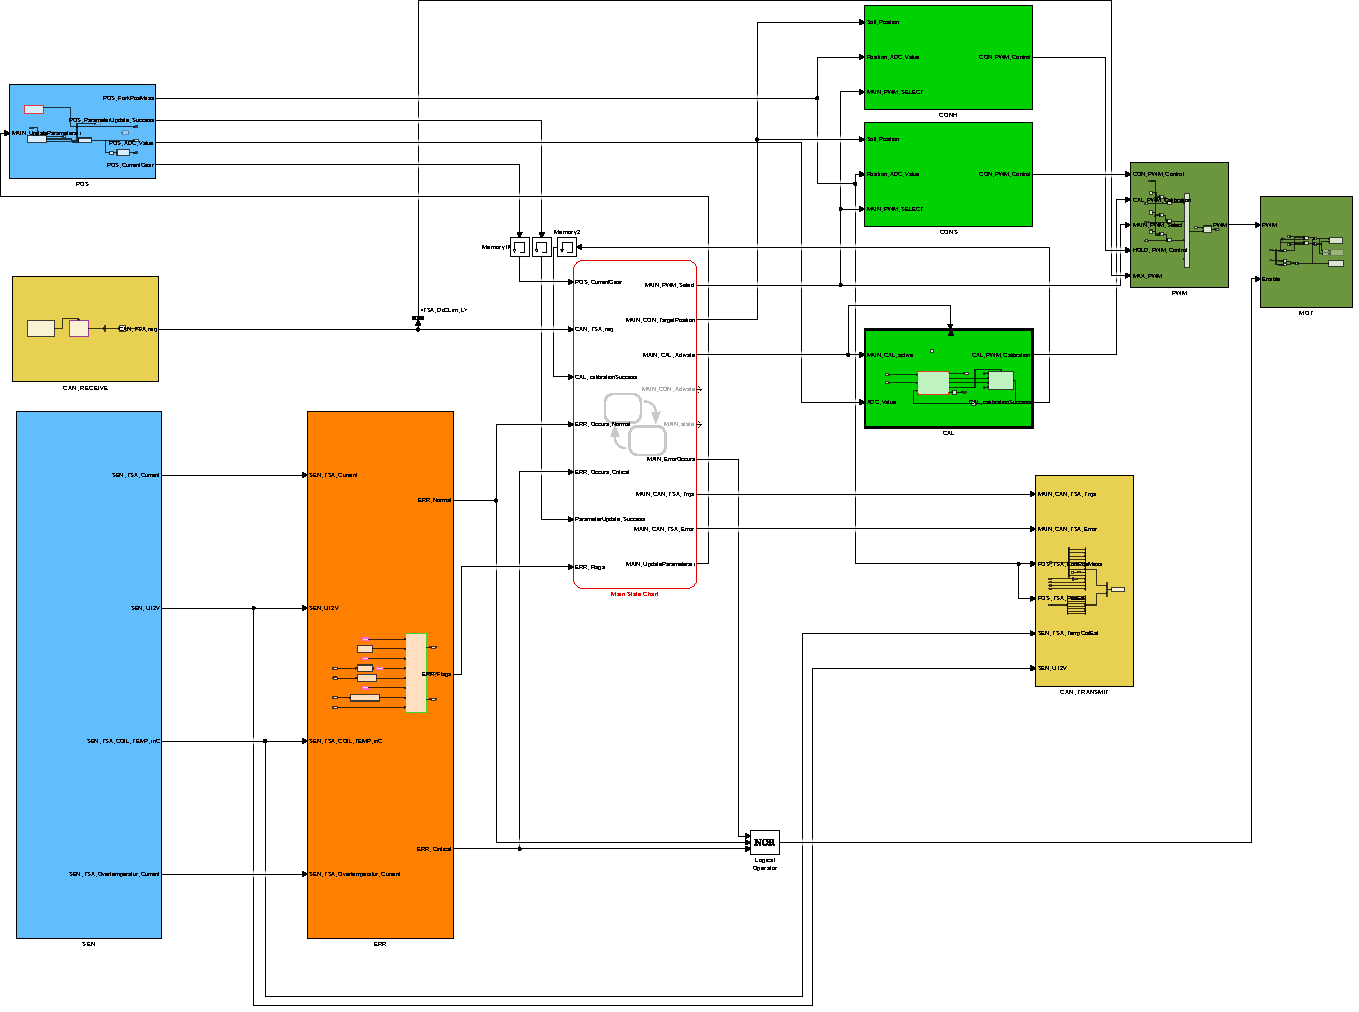
\includegraphics[width=0.9\columnwidth]{./Bilder/fig_gesamtsystem}%
\caption{Darstellung des Gesamtsystems}%
\label{fig_gesamtsystem}%
\end{figure}
Im Folgenden wird der Hauptzustandsautomat und die reflexbasierten Komponenten einzeln erläutert.

\subsection{Hauptzustandsautomat (MAIN)}

\begin{figure}[H]%
\centering
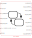
\includegraphics[width=0.6\columnwidth]{./Bilder/fig_main}%
\caption{Hauptzustandsautomat (MAIN), Außenansicht}%
\label{fig_main}%
\end{figure}

Der Hauptzustandsautomat ist die Kernkomponente der Software und beeinflusst jede Komponente des Systems. Als Eingangssignal wird dem Hauptzustandsautomaten
\begin{itemize}
	\item der aktuell eingelegte Gang (\textit{POS\_CurrentGear}),
	\item die letzte empfangene \textit{Trqs}-CAN-Nachricht (\textit{Main\_CAN\_TSA\_Trqs}),
	\item das Statussignal einer laufenden/abgeschlossenen Kalibrierung (\textit{CAL\_calibrationSuccess}),
	\item das Fehlersignal bei \textit{normalen Fehlern} (\textit{ERR\_Occurs\_Normal}),
	\item das Fehlersignal bei \textit{kritischen Fehlern} (\textit{ERR\_Occurs\_Ciritcal}),
	\item das Statussignal beim Laden der Kalibrierparameter (\textit{ParameterUpdate\_Success}) und
	\item eine Liste an Fehler Bits (\textit{ERR\_Flags})
\end{itemize}
zugeführt. Als Ausgangssignal gibt der Hauptzustandsautomat
\begin{itemize}
	\item die aktuelle Quelle für PWM Generierung (\textit{MAIN\_PWMS\_Select}),
	\item den Wunschgang (\textit{MAIN\_CON\_TargetPosition}),
	\item das Aktivierungssignal der Kalibrierung  (\textit{MAIN\_CAL\_Activate}),
	\item den aktuellen Zustand des Automaten  (\textit{MAIN\_state}),
	\item ein Fehlersignal bei internem Fehler im Automaten  (\textit{MAIN\_ErrorOccurs}),
	\item die \textit{Trqs}-CAN-Nachricht  (\textit{MAIN\_CAN\_TSA\_Trqs}),
	\item die \textit{Error}-CAN-Nachricht  (\textit{MAIN\_CAN\_TSA\_Error}) und
	\item den Auslöser zum Auslesen der Kalibrierparameter  (\textit{MAIN\_UpdateParameters()})
\end{itemize}
aus. Über \textit{MAIN\_PWMS\_Select} wird nicht nur die Quelle ausgewählt, die den Motortreiber ansteuert, sondern ebenfalls welche Teilsysteme aktiv sind. Somit wird sichergestellt, dass zu jedem Zeitpunkt ausschließlich ein einziger Regelalgorithmus oder Kalibrieralgorithmus ausgeführt wird (siehe dazu auch \autoref{performanceopt}).\\
Intern agiert der Zustandsautomat in vier streng separierten Betriebsmodi. Nach jedem Reset (bspw. nach dem Anlegen der Versorgungsspannung) befindet sich der Automat zunächst im Initialisierungsschritt. Hier werden zunächst für die Ausführung relevante Variablen initialisiert. Daran anschließend werden die Kalibrierparameter aus dem nichtflüchtigen Speicher geladen. Das Auslesen und Zwischenspeichern der Werte findet dabei im Block zur Schaltgabelpositionsermittlung (POS) statt und wird durch das Setzen eines entsprechenden Triggersignals angestoßen. Durch die Kalibrierwerte ist es nun möglich die aktuelle Schaltgabelposition zu bestimmen, wobei zunächst im Betriebsmodus \textbf{Inaktiv} verblieben wird. Durch einen entsprechenden CAN-Befehl kann der Übergang in den Betriebsmodus \textbf{Regulär} erfolgen. Hierin ist es möglich Schaltbefehle auszuführen. Es wird unterschieden zwischen \textit{Schalte in Gang X} und \textit{Bleibe in Gang X}, wobei jeweils entweder der Regler zum Schalten oder der Regler zum Halten der Position aktiv ist. Für Letzteren existiert noch keine zufriedenstellende Realisierung. Falls eine Kalibrierung durchgeführt werden soll, kann aus diesem Betriebsmodus in den Betriebsmodus \textbf{Kalibrierung} gewechselt werden. Aus allen Betriebsmodi wird durch das Auftreten eines Fehlers (angezeigt durch die entsprechenden Eingangssignale am Automaten) direkt in den Betriebsmodus \textbf{Fehler} übergegangen. In diesem Betriebsmodus werden keine Stellgrößen am Motortreiber zugelassen und alle Regler sind deaktiviert. Erst durch das Senden des entsprechenden Freigabe-Befehls wird wieder in den Betriebsmodus \textbf{Inaktiv} geschaltet.
 
\begin{figure}[H]%
\centering
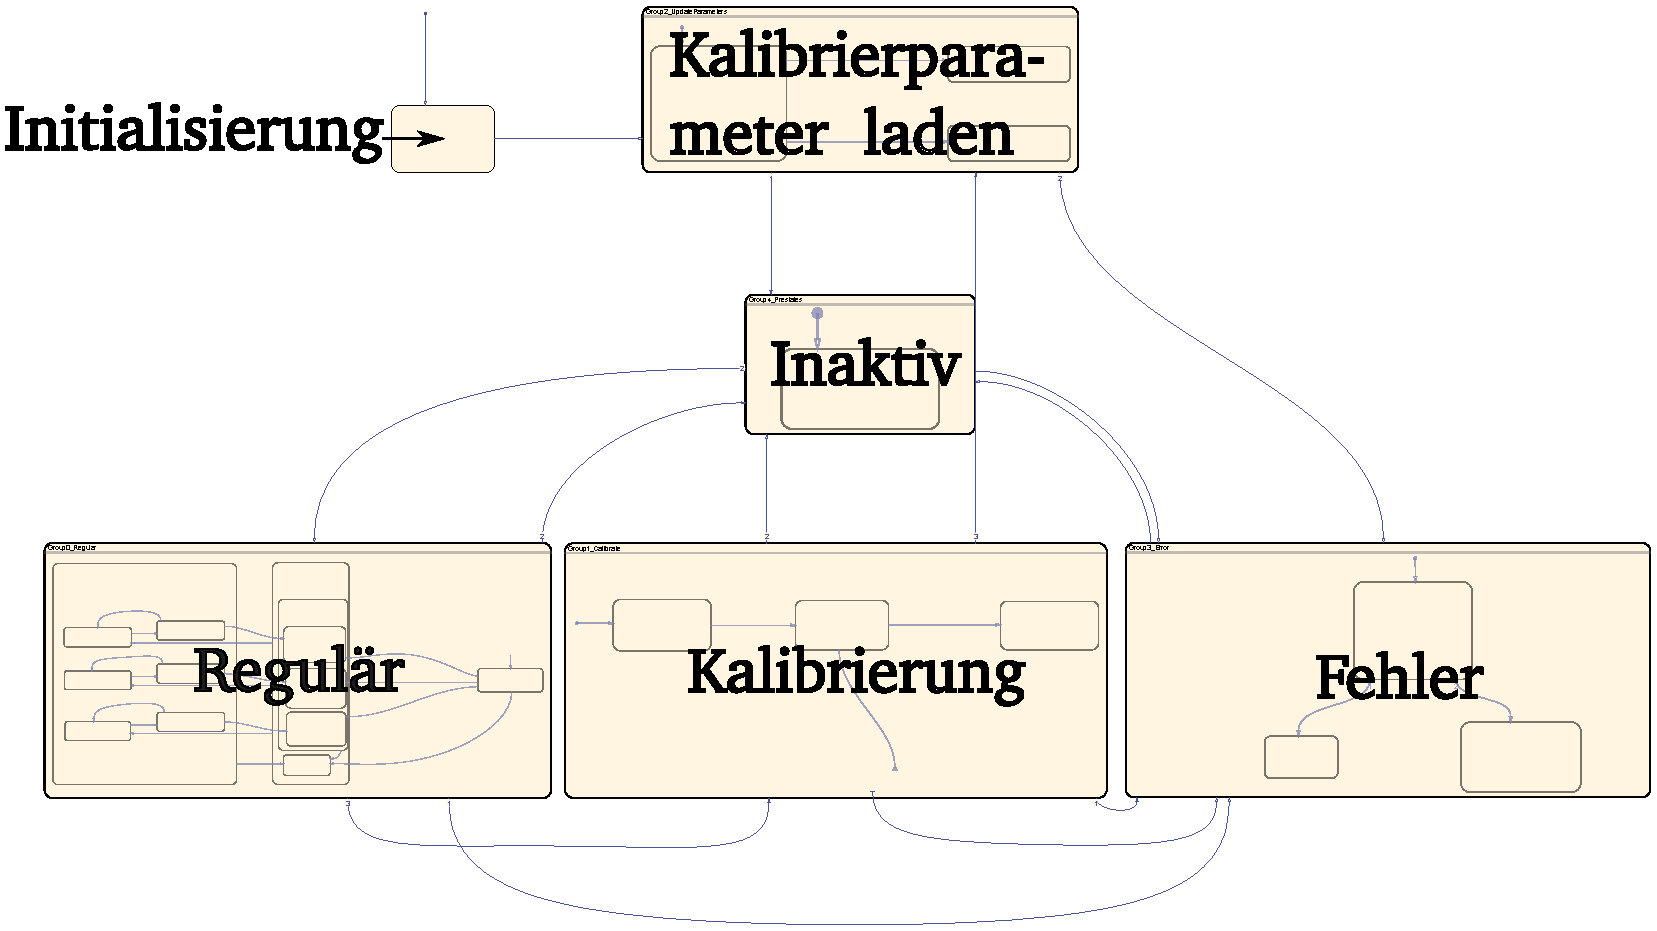
\includegraphics[width=0.6\columnwidth]{./Bilder/fig_main_detail}%
\caption{Hauptzustandsautomat (MAIN), vereinfachter Aufbau}%
\label{fig_main_detail}%
\end{figure}

\subsection{Positionsermittlung (POS)}\label{lagesens}
\begin{figure}[H]%
\centering
\includegraphics[width=0.3\columnwidth]{./Bilder/fig_POS}%
\caption{Schaltgabelpositionsermittlung}%
\label{fig_POS}%
\end{figure}

Die Positionsermittlung der Schaltgabel genießt eine Sonderstellung unter der Sensorik. Sie stellt die Regelgröße dar und ist daher von essentieller Bedeutung für die Regelung.  Dementsprechend wird die Positionsregelung getrennt von der restlichen Sensorik behandelt. Die Sensorik ist im \textit{SEN}-Subsystem anzutreffen (siehe \autoref{SEN}). Eingangsseitig kann durch den Hauptzustandsautomaten angestoßen werden, dass die Kalibrierdaten für die Lagesensorik aus dem nichtflüchtigen Speicher gelesen werden. Ausgangsseitig wird 
\begin{itemize}
	\item die momentane Gabelposition in Millimetern,
	\item der Zustand des Lesezugriffs auf die Kalibrierdaten,
	\item die Sensor Rohdaten und 
	\item der aktuell eingelegte Gang
\end{itemize}
bereit gestellt. 
Die Positionsmessung wird intern über einen ADC realisiert, durch den die Ausgangsspannung des Hall-Sensors (vgl. \autoref{regler}) in die Schaltgabelposition übersetzt wird. Um die Genauigkeit zu erhöhen wird sowohl der direkte als auch der komplementäre Sensorausgang erfasst. Somit wird eine Genauigkeit von \SI{0,1}{mm} erzielt. Durch eine \textit{Burst}-Messung kann die Genauigkeit noch weiter erhöht werden. Hierbei werden mehrere Messungen durchgeführt und in einen Puffer zwischengespeichert ohne den Programmablauf zu unterbrechen. In regelmäßiger Auslesefrequenz wird die gepufferte Menge an Sensordaten durch das Programm ausgelesen und verarbeitet. Im STM32 wird diese Funktion über \textit{Direct Memory Access} realisiert, wodurch die ADC-Peripherie Messwerte direkt in den Speicher schreibt, den der Prozessor in regelmäßigen Abständen ausließt \cite{stm32}. Diese Funktion wird in \autoref{perfVergl} wieder aufgegriffen.

\subsection{CAN-Kommunikation (CAN\_RECEIVE, CAN\_TRANSMIT)}

\begin{figure}[H]%
\centering
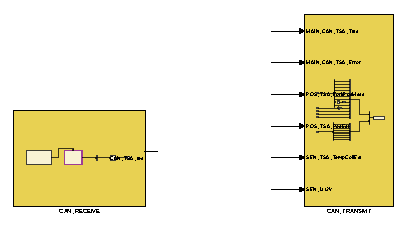
\includegraphics[width=0.6\columnwidth]{./Bilder/fig_can}%
\caption{CAN-Kommunikation}%
\label{fig_can}%
\end{figure}

Die CAN-Kommunikation wird durch eine Empfangs- (\textit{CAN\_RECEIVE}) und eine Sendekomponente (\textit{CAN\_TRANSMIT}) realisiert. Die Empfangskomponente funktioniert Interrupt-basiert und wird somit immer aktiv, wenn eine neue Nachricht empfangen wird. Über einen Rate-Transmission-Block wird diese Empfangsfrequenz an die Arbeitsfrequenz des Hauptzustandsautomaten angepasst. Als Ausgang steht dem Automaten ein Bus-Vektor mit dem Nachrichteninhalt zur Verfügung. 
Die Sendekomponente basiert auf \textit{Non-Blocking}-Basis. Dadurch können während des Sendevorgangs nebenläufig auch noch andere Aufgaben abgearbeitet werden. Die einzelnen Eingangswerte werden vor dem Senden zu größeren Nachrichten zusammengefügt.

\subsection{Sensorik (SEN)}\label{SEN}
\begin{figure}[H]%
\centering
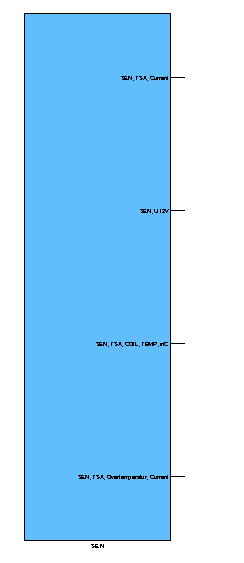
\includegraphics[width=0.3\columnwidth]{./Bilder/fig_sen}%
\caption{Sensorik}%
\label{fig_sen}%
\end{figure}
Die Sensorik umfasst eine Strommessung durch den Aktor, eine Spannungsmessung am Eingang, eine Spulentemperaturmessung und eine Detektion gegen Übertemperatur/Überstrom an den Halbbrücken. Die Sensorwerte stehen zunächst als ADC-Rohwerte für die weitere Verarbeitung bereit. Diese werden je nach Sensortyp skaliert oder wie im Falle des externen Thermistors durch komplexe Formeln in den realen Messwert konvertiert (vgl. \autoref{ch:komp}). An den Ausgängen stehen anschließend die Messgrößen in gewünschter Einheit bereit. Der Lagesensor wird nach \autoref{lagesens} implementiert.

\subsection{Fehlererkennung (ERR)}\label{err}
\begin{figure}[H]%
\centering
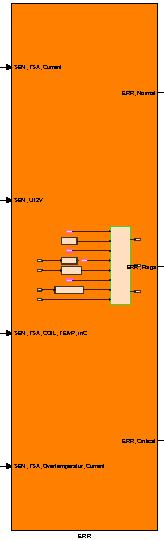
\includegraphics[width=0.25\columnwidth]{./Bilder/fig_err}%
\caption{Fehlererkennung}%
\label{fig_err}%
\end{figure}
Durch die Fehlererkennung werden die gemessenen Überwachungsgrößen mit Schwellwerten verglichen und ggf. ein Fehlersignal zum Hauptzustandsautomaten weitergeleitet. Dabei muss berücksichtigt werden, dass Messfehler erkannt und ggf. gefiltert werden und nicht zu falsch positiv Ergebnissen führen. Auf der anderen Seite sollten Fehler schnellstmöglich erkannt werden und die falsch negativ - Rate minimal sein. Neben dem Hauptzustandsautomaten besitzt die Komponente auch noch eine Schnittstelle zum Motortreiber, um den Stromfluss im Aktor schnellstmöglich zu unterbinden. Hierfür wird das in \autoref{subsec:MOT} genauer erklärte \textit{enable}-Signale genutzt. \\
Eine Sonderstellung nimmt der Systemfehler (\textit{TSA\_SystErr}) ein, der bei Fehlern im Softwaresystem auftritt. Dazu zählen Zustände, die nie erreicht werden sollten und ausschließlich zur Fehlererkennung dienen. Das Erreichen der Zustände deutet auf einen Programmierfehler und/oder eine nicht berücksichtigte Situation hin. Durch einen CAN-Befehl zur Fehlerfreigabe, wird das Softwaresystem wieder in den Initialzustand versetzt.

\subsection{Kalibrierung (CAL)}

\begin{figure}[H]%
\centering
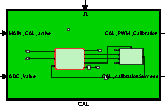
\includegraphics[width=0.35\columnwidth]{./Bilder/fig_cal}%
\caption{Kalibrierung (Lagesensor)}%
\label{fig_cal}%
\end{figure}

Die Kalibrierung dient dazu, den Spannungswerten des Lagesensors konkrete Positionen der Schaltgabel zuordnen zu können. Das Kalibrierungsverfahren basiert auf dem Ansatz von \cite{adp}. Es werden dabei die Anschlagspositionen durch große Stellgrößen angefahren und der Sensor an diesen Werten ausgelesen. Nach mehrmaliger Ausführung und anschließender Mittlung werden die Kalibrierungswerte nichtflüchtig abgespeichert. Im Falle eines Spannungsverlustes stehen die Kalibrierungsdaten nach wie vor bereit. Die Komponente besitzt Schnittstellen zur Lagesensorik sowie zum Hauptzustandsautomaten, von welchem aus die Kalibrierung eingeleitet wird.

\subsection{Halteregler (CONH) und Schaltregler (CONS)}

\begin{figure}[H]%
\centering
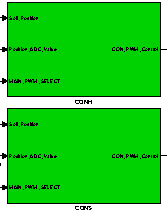
\includegraphics[width=0.3\columnwidth]{./Bilder/fig_conh_cons}%
\caption{Regelung}%
\label{fig_conh_cons}%
\end{figure}

Für die Regelung der Schaltgabelposition nach \autoref{regler} werden den Reglern die momentane Gabelpositon zugeführt. Darüber hinaus wird über den Hauptzustandsautomaten die Sollposition vorgegeben. Über den Soll-Ist-Vergleich und die Anwendung eines Regelgesetzes wird schließlich eine PWM als Stellgröße ermittelt. Eine Regelfrequenz von \SI{10}{kHz} hat sich als ausreichend schnell herausgestellt und kann durch den Mikrocontroller geleistet werden. Beim \textit{Schaltregler} kommt ein PID-Regler mit Störgrößenkompensation zum Einsatz, der in \cite{adp} erarbeitet wurde. Eine praktikable Lösung für einen \textit{Halteregler} konnte nicht ermittelt werden. Der jeweilige Regler ist nur aktiv, falls er durch den \textit{MAIN\_PWM\_SELECT} des Hauptzustandsautomaten auch explizit angefragt ist.
 
\subsection{Auswahlglied für PWM-Signal (PWMS)}

\begin{figure}[H]%
\centering
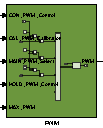
\includegraphics[width=0.25\columnwidth]{./Bilder/fig_pwm}%
\caption{Auswahlglied für PWM-Signal}%
\label{fig_pwm}%
\end{figure}

Über das Auswahlglied für das PWM-Signal wird selektiert, welche der möglichen PWM-Signale zum Motortreiber durchgeschaltet wird. Die Auswahl wird aufgrund des \textit{MAIN\_PWM\_SELECT}-Eingangs getroffen. Darüber hinaus kann die maximale PWM durch entsprechende CAN-Signale begrenzt werden. 

\subsection{Motortreiber (MOT)} \label{subsec:MOT}

\begin{figure}[H]%
\centering
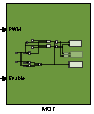
\includegraphics[width=0.10\columnwidth]{./Bilder/fig_mot}%
\caption{Motortreiber}%
\label{fig_mot}%
\end{figure}

Der Motortreiber erwartet ein vorgegebenes PWM-Signal, bzw. dessen Tastgrad \textit{p}. Über das Vorzeichen wird bestimmt, welche der beiden Halbbrücken gepulst angesteuert wird und welche konstant auf Erdpotential gesetzt wird. Über ein explizites \textit{enable}-Signal kann der Motortreiber bspw. im Falle einer Notausschaltung deaktiviert werden. Hierfür wird der Motortreiber über einen separaten Pin in einen \textit{sleep mode} gesetzt (vgl. \autoref{sec:hbridge}). Zwei Vorgabewerte werden demnach in Signale umgewandelt, die zur H-Brücke weitergeführt werden.


\section{Codegenerierung und Performanceoptimierung} \label{performanceopt}
Der generierte und kompilierte Code wird auf dem Mikroprozessor Cortex M4 ausgeführt, der auf dem STM32F4 eingesetzt wird. Dieser Mikroprozessor zeichnet sich durch eine vergleichsweise hohe Rechenleistung aus und verfügt darüber hinaus über eine \textit{Floating Point Unit} (FPU). Somit ist er in der Lage Gleitkommazahlen zu verrechnen. Bei maximaler Taktfrequenz ist die Rechenleistung begrenzt auf \SI{225}{DMIPS}. In DMIPS wird dabei die Leistungsfähigkeit, gemessen an einem repräsentativen Testprogramm namens \textit{Dhrystone}, angegeben \cite{dmips}. Der Prozessor kann daher nicht beliebig viele Aufgaben in beliebiger Arbeitsfrequenz abarbeiten. Für weiterführende Informationen sei auf das Datenblatt \cite{stm32} verwiesen.\\
Um zu verstehen, wie die begrenzten Rechenressourcen optimal ausgelastet werden können, ist es von Vorteil den Codegenerierungsprozess zu kennen. Über Waijung und die Simulink Toolboxes wird Code nach dem sogenannten \textit{Multirate Single Tasking}- Prinzip generiert. Somit ist es möglich, mehrere Aufgaben mit unterschiedlichen Arbeitsfrequenzen abzuarbeiten.  Über den sogenannten \textit{SysTick Timer} wird in der Frequenz der höchstfrequenten Aufgabe ein Interrupt ausgelöst. Ein Interrupt bezeichnet eine Unterbrechung des regulären Programmablaufs, wobei nach der Abarbeitung der sogenannten Interrupt Service Routine wieder der reguläre Programmablauf an der letzten Stelle fortgeführt wird. 
Innerhalb des \textit{SysTick Timer}-Interrupts wird angestoßen, dass diejenigen Aufgaben ausgeführt werden, die zum entsprechenden Zeitpunkt ausgeführt werden sollen. Beispielsweise wird eine Aufgabe, die mit \SI{100}{Hz} ausgeführt werden soll, durch jeden zehnten \textit{SysTick Timer}-Interrupt mit \SI{1}{kHz} angestoßen. Eine Besonderheit fallen Aufgaben zu, die als laufzeitkritisch eingestuft werden, denn diese Aufgaben werden direkt innerhalb der Interrupt Service Routine abgearbeitet und haben somit Priorität vor den übrigen Aufgaben. Ein Beispiel einer solchen Aufgabe ist der geschlossene Regelkreis zur Reglung der Gabelposition. Um den Ablauf des Programms nicht zu gefährden, muss darauf geachtet werden, dass diese Aufgaben nicht länger dauern als bis zum Auslösen des nächsten \textit{SysTick Timer}-Interrupts. Zusätzlich muss noch genügend Zeit bleiben, um die übrigen Aufgaben auszuführen.\cite{waijung}\\
Um dies zu ermöglichen wird eine Reihe von Maßnahmen ergriffen, die im Folgenden kurz vorgestellt werden.
Zunächst sind ausschließlich Teile des Systems aktiv, die zum aktuellen Zeitpunkt auch benötigt werden. Alle Funktionalitäten zur Kalibrierung, Halteregelung und Speicherung nichtflüchtiger Daten sind beispielsweise während eines Schaltvorgangs deaktiviert. So wird verhindert, dass wartende inaktive Prozesse Rechenzeit beanspruchen.
Als weitere Maßnahme wird die Arbeitsfrequenz für verschiedene streng voneinander geteilte Bereiche evaluiert, sodass jeder Bereich nur so oft wie nötig aufgerufen wird.
Auch durch die Wahl entsprechender Variablentypen kann die Gesamtperformance optimiert werden. Viele Mikrocontroller bieten keine FPU und können demnach hardwarebeschleunigt keine Gleitkommaoperationen durchführen (vgl. STM32F0, STM32F1). Daher werden in solchen Fällen statt Gleitkommazahlen Festkommazahlen oder eine Skalierung auf Ganzzahlen verwendet. Da der STM32F4 jedoch über eine FPU verfügt, ist der Leistungsgewinn in dieser Hinsicht begrenzt. Wichtig ist jedoch zu berücksichtigen, dass der STM32 einen 32-bit Prozessor besitzt und die Arithmetische Logik Einheit (ALU) nur Zahlen im 32-bit Bereich direkt verrechnen kann. Auf 64-bit Zahlen wird daher im Unterschied zu modernen 64-bit-Architekturen verzichtet, auch wenn sie einen höheren Zahlenbereich bzw. eine höhere Genauigkeit bei Gleitkommazahlen besitzen \cite{stm32}.
Neben des Programms als solches kann auch der Mikrocontroller in seiner Leistungsfähigkeit maximiert werden. Naheliegend ist dabei die Kern-Taktfrequenz so weit wie möglich zu erhöhen, damit in gleicher Zeit mehr Befehle abgearbeitet werden können. Dies setzt voraus, dass eine ausreichend hohe Versorgungsspannung angelegt wird. Ein Zusammenhang zwischen maximaler Taktfrequenz und dafür benötigter Versorgungsspannung ist in \cite{stm32}gegeben. Bei zu hoher Taktfrequenz bei zu geringer Versorgungsspannung, sind Instabilitäten nicht auszuschließen, was den Betrieb des Schaltaktors gefährden würde. Der Kerntakt (FCLK), über welchen die Rechengeschwindigkeit beeinflusst wird, leitet sich aus dem sogenannten Clocktree aus \autoref{fig_clock} ab. In diesem können auch zahlreiche weitere Taktraten eingestellt werden wie der für die ADCs relevante \textit{APB Peripheral Clock}. Es stehen verschiedene Taktgeber zur Verfügung, aus denen die Takte abgeleitet werden können. Im vorliegenden Fall wird ein externer Schwungquarz an \textit{High Speed External} (HSE) verwendet. \cite{stmref} \\

\section{Performancevergleich zu vorherigen Ansätzen} \label{perfVergl}
Für das Programm wird bei maximaler Kerntaktfrequenz von \SI{168}{MHz} eine Regelfrequenz von \SI{10}{kHz} erreicht. Es wird demnach in einem Abstand von \SI{100}{\mu s} ein Soll-/Ist-Vergleich der Gabelposition durchgeführt, darauf das Regelgesetz angewendet und anschließend der resultierende Stellwert an den Motortreiber weitergegeben. Im Vergleich zum vorherigen Ansatz mit MicroAutoBox ist somit eine um den Faktor $10$ höhere Regelfrequenz möglich (vgl. \cite{adp}). Hierbei muss jedoch beachtet werden, dass die Programme nicht identisch sind. Während im vorliegenden Programm zahlreiche Zusatzfunktionalitäten neben der eigentlichen Regelung bereitgestellt werden, werden auf der MicroAutoBox zusätzliche Berechnungen zur sensorlosen Messungen angestellt. \\
Vorteile besitzt der Mikrocontroller weiterhin in der hohen Abtastrate seiner ADCs, was nach \cite{adp} für eine sensorlose Positionsermittlung zwingend notwendig ist. Im sogenannten \textit{triple interleaved mode} sind bis zu \SI{7,2}{MSPS} (Millionen Abtastungen pro Sekunde) möglich, wobei alle drei ADCs des STM32 versetzt einen Eingang abtasten. Jeder einzelne ADC tastet demnach mit bis zu \SI{2,4}{MSPS} ab \cite{stm32}. Die MicroAutoBox ist auf \SI{1,25}{MSPS} beschränkt und tastet demnach wesentlich langsamer ab. \\
Berücksichtigt werden muss jedoch, dass eine \textit{Burst}-Messung, wie sie in \cite{adp} verwendet wird, nicht nativ unter Waijung  unterstützt wird. Um zusätzlich das volle Potential der ADCs auch unter Waijung auszuschöpfen, kann ein weiterer \textit{Custom-Block} in C programmiert werden, der eine \textit{Burst}-Messung realisiert. Damit ist der ADC des STM32 der MicroAutobox überlegen und würde den Anforderungen aus \cite{adp} entsprechen.  \\
Im Fall mit Sensor kann auf eine \textit{Burst}-Messung aufgrund ausreichender Genauigkeit verzichtet werden, daher wird auf den nativen Block zurückgegriffen. Die sich aus den genannten Vorteilen ergebenen Verbesserungen bei der Ausregelung werden in \autoref{reglerergebnisse} thematisiert.

\begin{figure} [H]%
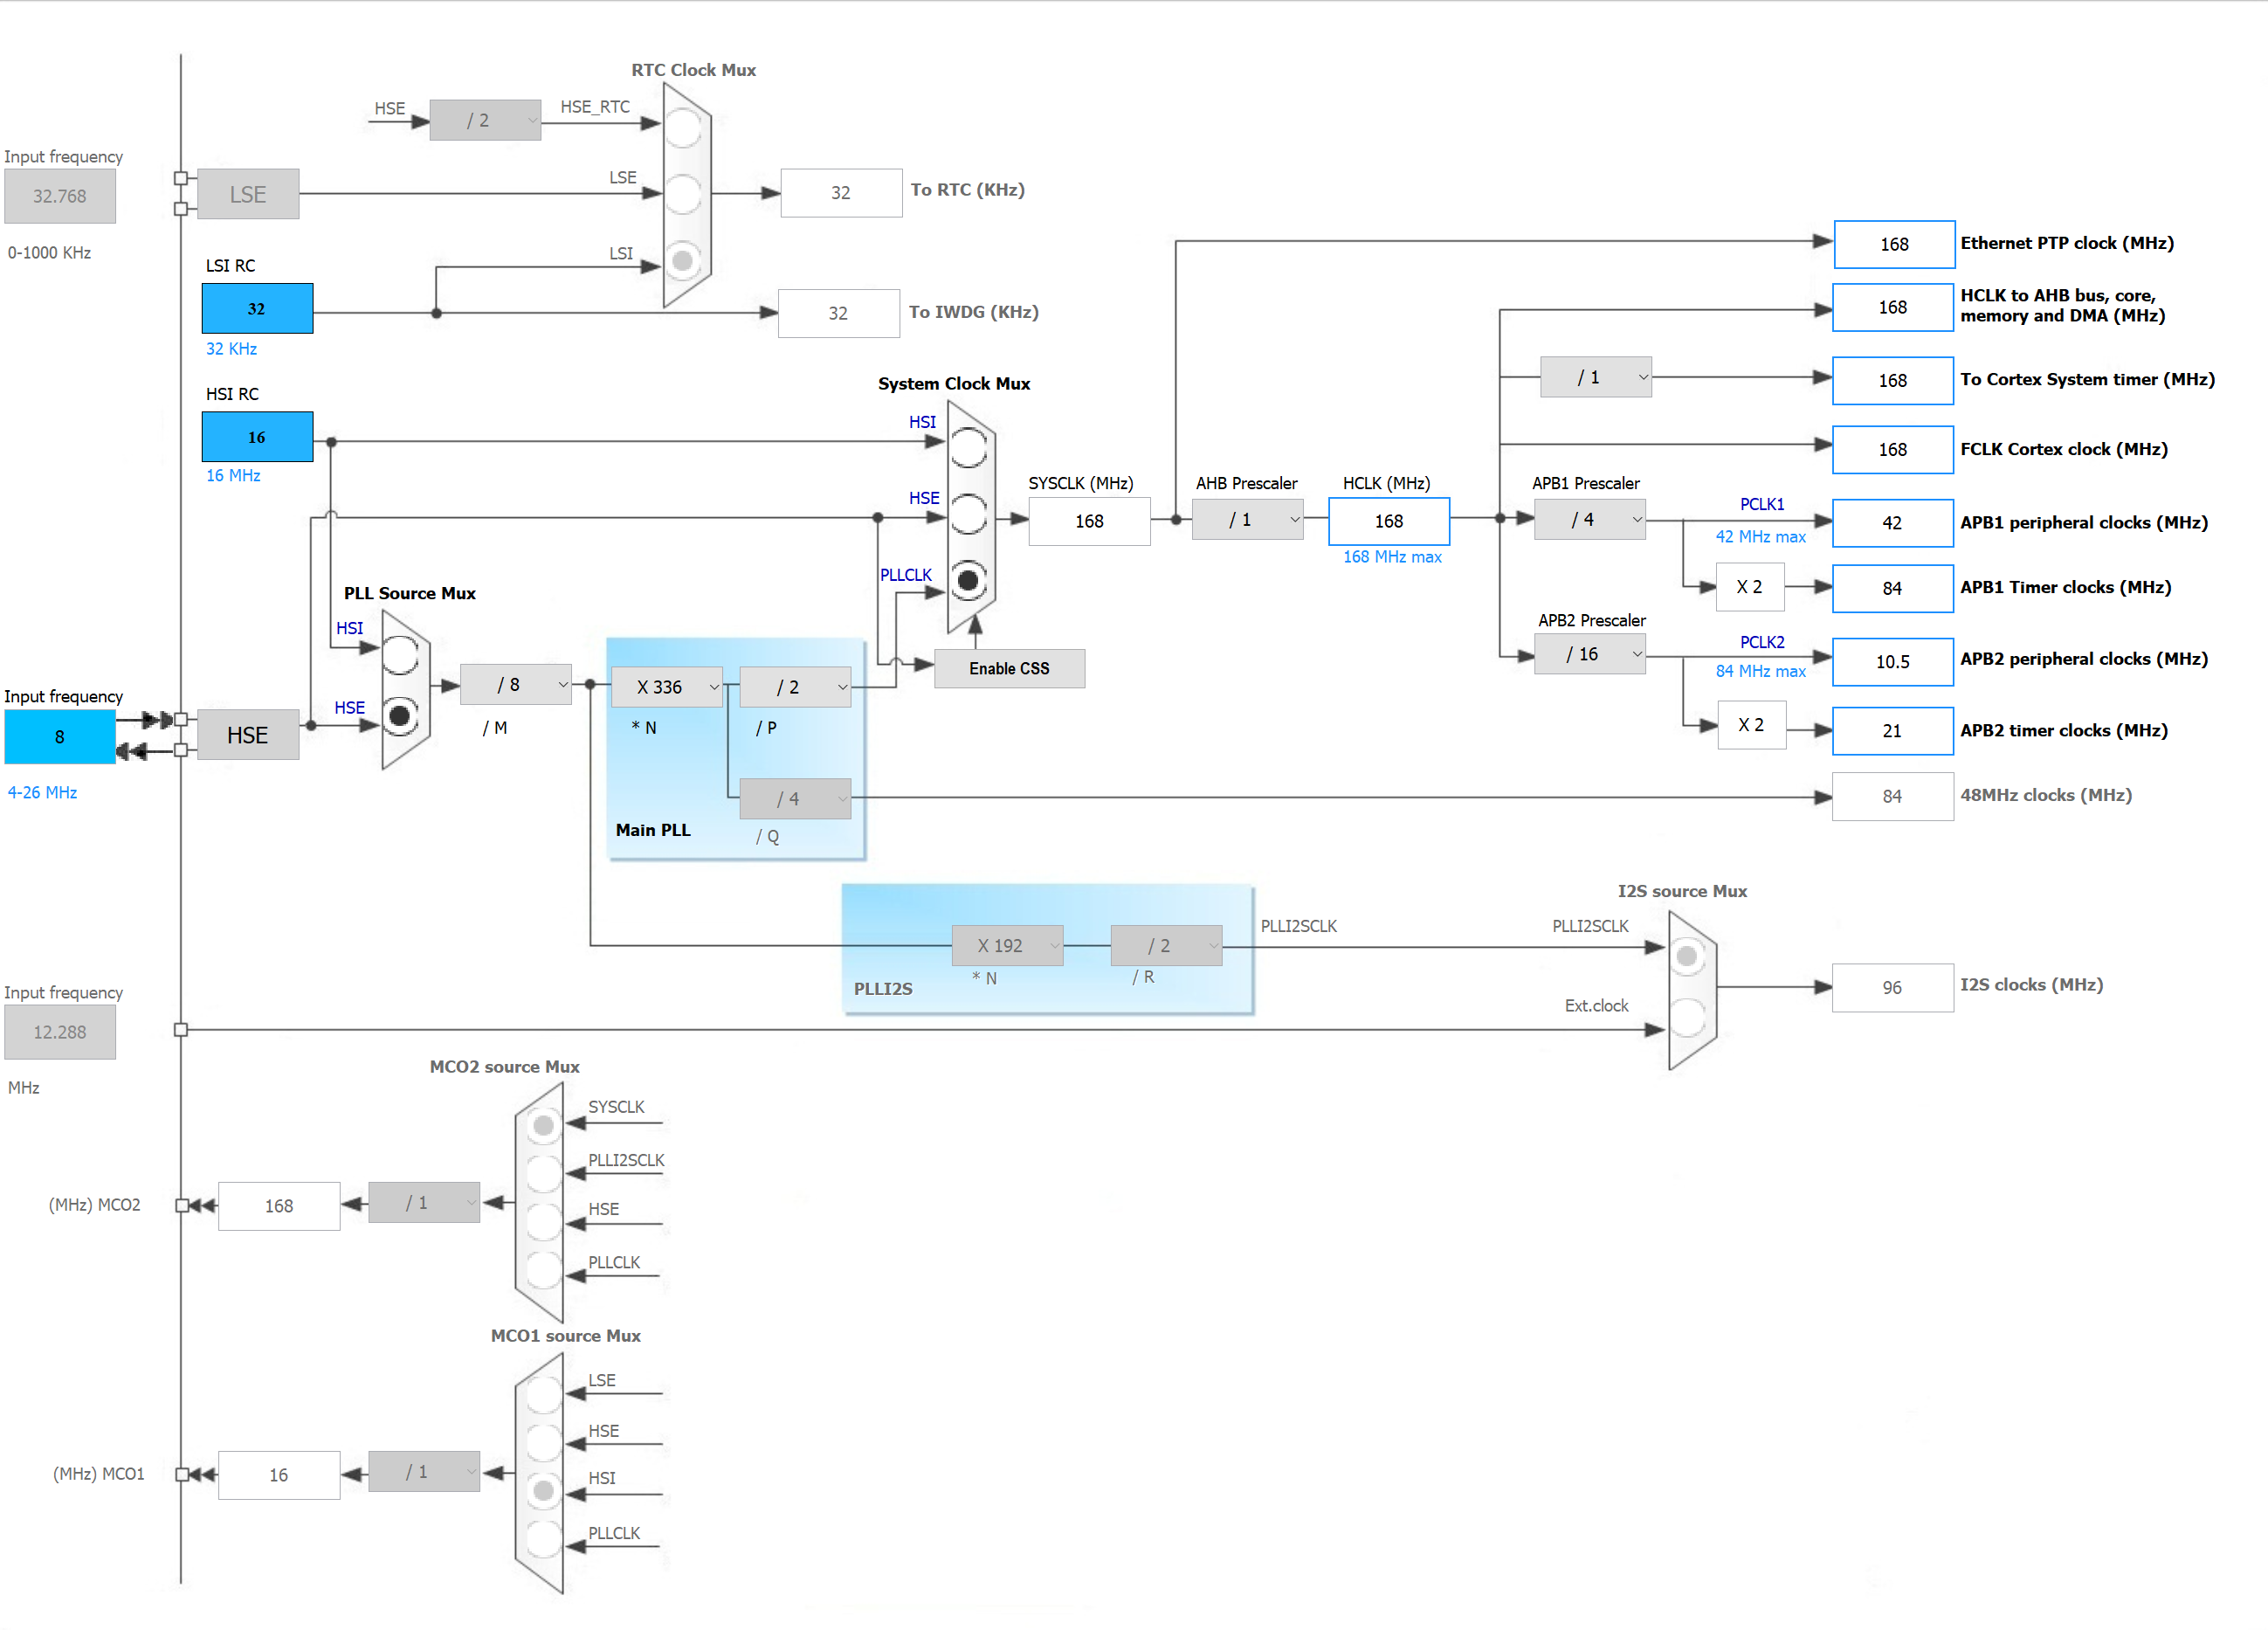
\includegraphics[width=\columnwidth]{./Bilder/fig_clock}%
\caption{Taktbaum generiert in STM32 CubeMX}%
\label{fig_clock}%
\end{figure}

\section{Einleitung in benutzerseitige CAN Schnittstelle} \label{CANNachrichten}

\begin{figure}[H]%
\centering
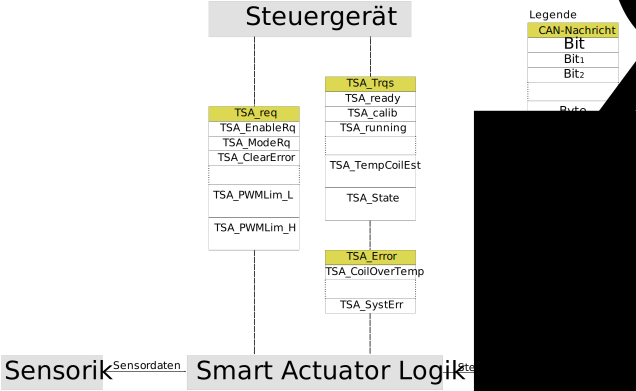
\includegraphics[width=1.0\columnwidth]{./Bilder/fig_can_ov}%
\caption{Gesamtkonzept der CAN-Kommunikation}%
\label{fig_can_ov}%
\end{figure}

Für den späteren Anwender ist vornehmlich die Benutzerschnittstelle über CAN relevant. Hier wird zunächst zwischen drei Nachrichten unterschieden, die innerhalb des CAN-Netzwerkes fortlaufend ausgetauscht werden. Über die Nachricht \textit{TSA\_req}, die in \autoref{tab_tsa_req} beschrieben ist, kann ein übergeordnetes Steuergerät Befehle an den Aktor schicken. Diese werden dann abhängig des aktuellen Zustands entsprechend umgesetzt. Parallel werden vom Aktor permanent Nachrichten an das Steuergerät gesendet, die Informationen über den aktuellen Zustands liefern. Dabei werden die Informationen auf zwei Nachrichten aufgeteilt, genaueres ist \autoref{tab_tsa_trqs} und \autoref{tab_tsa_error} zu entnehmen. Das Gesamtkonzept ist in \autoref{fig_can_ov} dargestellt.

\begin{table}%
\centering
\begin{tabular}{l c p{6cm} p{4cm}}
\hline
Bezeichnung & Datentyp & Erläuterung & Zusatz \\
\hline
TSA\_EnableRq & Bit & Aktivierungssignal des Aktors & Durch Setzen dieses Bits wird von Betriebsmodus \textbf{Inaktiv} zu \textbf{Regulär} gewechselt \newline \\
TSA\_ModeRq & Bit & Wahl des gewünschten Betriebsmodus \textbf{Regulär} oder  \textbf{Kalibrierung }, über dieses Signal kann die Kalibrierung gestartet werden \newline & 0: Regulär, 1: Kalibrierung \newline \\
TSA\_ClearError & Bit & Fehler Quittierung & Durch Setzen wird von Betriebsmodus \textbf{Fehler} zu \textbf{Inaktiv} gewechselt, falls der Fehler behoben wurde \newline \\
TSA\_ShiftFirst & Bit & Schaltbefehl in ersten Gang & nur möglich in Betriebsmodus \textbf{Regulär} \newline\\
TSA\_ShiftSecond & Bit & Schaltbefehl in zweiten Gang & nur möglich in Betriebsmodus \textbf{Regulär} \newline \\
TSA\_ShiftNeutral & Bit & Schaltbefehl in neutrale Position & nur möglich in Betriebsmodus \textbf{Regulär} \newline \\
TSA\_PWMLim\_L & unsigned Byte & Obere Grenze für PWM - Puls/Pausen- Verhältniss & Low Byte \newline \newline \\
TSA\_PWMLim\_H & unsigned Byte & Obere Grenze für PWM - Puls/Pausen- Verhältniss & High Byte \\
\end{tabular}
\caption{Erläuterung der CAN-Nachricht \textit{TSA\_req}}
\label{tab_tsa_req}
\end{table}

\begin{table}%
\centering
\begin{tabular}{l c p{6cm} p{4cm}}
\hline
Bezeichnung & Datentyp & Erläuterung & Zusatz \\
\hline
TSA\_ready & Bit & Aktor ist betriebsbereit & Aktor befindet sich weder im Fehler- noch im Initialisierungszustand \newline \\
TSA\_calib & Bit & Laufender Kalibriervorgang & - \newline \\
TSA\_running & Bit & Warten auf Befehle & Aktor befindet sich in Betriebsmodus \textbf{Regulär} \newline \\
TSA\_shifting & Bit & Laufender Schaltvorgang & Es können keine weiteren Schaltbefehle entgegen genommen werden \newline\\
TSA\_firstGearEng & Bit & Erster Gang eingelegt & Gangposition erkannt und in gültigem Toleranzbereich \newline \\
TSA\_secondGearEng & Bit & Zweiter Gang eingelegt & Gangposition erkannt und in gültigem Toleranzbereich \newline \\
TSA\_neutralGearEng & Bit & Neutrale Gangposition eingelegt & Gangposition erkannt und in gültigem Toleranzbereich \newline \\
TSA\_Heartbeat& Bit & Lebenszeichen im Sekundentakt & Gibt Auskunft über funktionierenden Programmablauf \newline \newline \\
TSA\_Error & Bit & Fehlerzustand & Aktor in Betriebsmodus \textbf{Fehler}, Informationen liefert \textit{TSA\_Error} \newline \\
TSA\_ForkPosMeas & unsigned Byte & Aktuelle Schaltgabelposition & Gemessen in Millimetern \newline \\
TSA\_DcInput & unsigned Byte & Aktuelle Eingangsspannung & Gemessen in V \newline \\
TSA\_TempCoilEst & unsigned Byte & Aktuell gemessene Spulentemperatur & Gemessen in Grad Celsius, um +100 Offsetverschoben \newline \\
TSA\_State & unsigned Byte & Momentaner Zustand in Hauptzustandsautomaten & ID des Zustands des Hauptzustandsautomaten (zur Fehleranalyse) \\
\end{tabular}
\caption{Erläuterung der CAN-Nachricht \textit{TSA\_Trqs}}
\label{tab_tsa_trqs}
\end{table}

\begin{table}%
\centering
\begin{tabular}{l c p{6cm} p{4cm}}
\hline
Bezeichnung & Datentyp & Erläuterung & Zusatz \\
\hline
TSA\_CoilOverTemp & Bit & Übertemperatur in Spulenwicklungen festgestellt & Schwellwert konfigurierbar über \textit{ERR\_limCoilTemp} \newline \\
TSA\_HbridgeOvertemp & Bit & Übertemperatur in H-Brücke festgestellt & Schwellwert konfigurierbar über \textit{ERR\_limHTemp} \newline \\
TSA\_CalibErr & Bit & Fehlerhafte Kalibrierung & Timeout überschritten, ungültige Kalibrierergebnisse oder fehlerhafte Langzeitspeicherung \newline \\
TSA\_dcVErr & Bit &  Eingangsspannungsbereich unter- oder überschritten & Schwellwert konfigurierbar über \textit{ERR\_dcLimMin} und \textit{ERR\_dcLimMax} \newline \\
TSA\_SensErr & Bit & Fehlerhafte Sensormesswerte & Sensorwerte außerhalb des erwarteten Bereichs oder inkonsistent \newline \\
TSA\_ShiftErr & Bit & Fehler bei Schaltvorgang & Timeout überschritten oder unerwarter schlechter Schaltverlauf \newline \\
TSA\_ShortCirc & Bit &  Überstromerkennung in Aktor & Schwellwert konfigurierbar über \textit{ERR\_limCurrent} \newline \\
TSA\_SystErr& Bit & Ein Systemfehler ist aufgetreten & Softwaresystem befindet sich in ungeplantem Zustand (vgl. \autoref{err}) und muss zurückgesetzt werden \newline \\

\end{tabular}
\caption{Erläuterung der CAN-Nachricht \textit{TSA\_Error}}
\label{tab_tsa_error}
\end{table}
\chapter{Analyse und Performance}\label{kap7}

\section{Beurteilung der Anforderungserfüllung}

\section{Kostenaufstellung}
Die Kosten für die fertige Platine inklusive aller Bauteile belaufen sich bei einer einzigen Platine auf 80 Euro. Bei einer Stückzahl von 100 kann der Preis bereits auf 33,5 Euro gesenkt werden, während die Bauteilkosten bei einer Fertigung von 1000 Platinen nochmal auf knapp unter 25 Euro sinken. Diesen großen Preisunterschied verursacht vor allem die unbestückte Platine selbst, die bei Bestellung von einer einzigen 38,5 Euro kostet und bei einer Bestellung von 1000 Stück nur noch 0,82 Euro. Tabelle \ref{tab:Preisliste} zeigt die verwendeten Bauteile und deren Anzahl sowie den kumulierte Preis pro Bauteilart (Anzahl des Bauteils multipliziert mit dem Einzelpreis) für jeweils eine Fertigung von einer Platine, von 100 Platinen und von 1000 Platinen. Die Preise stammen dabei von den Anbietern, bei denen die Komponenten jeweils eingekauft wurden.

\begin{table}[h]
	\centering
\begin{tabular}{ | l | l | l | l | l | }
\hline
	Anzahl & Bauteil & Bauteilpreis & Bauteilpreis 100+ & Bauteilpreis 1000+\\ \hline
	1 & Platine & 38.5 Euro & 2.39 Euro & 0.82 Euro\\
	\  & \  & \  & \  & \  \\
	1 & Mikrocontroller & 10.66 Euro & 7.79 Euro & 6.58 Euro \\
	2 & Halbbrücken & 6.56 Euro & 5.96 Euro & 5.04 Euro\\
	1 & Leitungstreiber & 0.617 Euro & 0.348 Euro & 0.252 Euro \\
	1 & CAN Transceiver & 2.82 Euro & 2.28 Euro & 1.51 Euro \\
	1 & Voltage Regulator 3,3V & 0.337 Euro & 0.162 Euro & 0.103 Euro \\
	1 & Voltage Regulator 5V & 0.337 Euro & 0.162 Euro & 0.103 Euro \\
	\  & \  & \  & \  & \  \\
	1 & Klemmblock & 1.16 Euro & 1.07 Euro & 0.912 Euro \\
	2 & Klemmblock & 0.742 Euro & 0.618 Euro & 0.526 Euro \\
	1 & Steckverbinder & 0.0442 Euro & 0,0442 Euro & 0,0387 Euro \\
	1 & AMPSEAL Automotive Steckverbinder & 7.09 Euro & 6.22 Euro & 5.23 Euro\\
	\  & \  & \  & \  & \  \\
	1 & Quarz & 0.605 Euro & 0.355 Euro & 0.384 Euro \\
	21 & Widerstände & 4.88 Euro & 3.046 Euro & 1.6754 Euro\\
	21 & Kondensatoren & 5.907 Euro & 3.0648 Euro & 1.501 Euro\\ \hline
	\  & \textbf{Gesamtpreis} & \textbf{80,26 Euro}  & \textbf{33,51 Euro}  & \textbf{24,68 Euro}  \\ \hline
\end{tabular}
\caption{Preisliste}
	\label{tab:Preisliste}
\end{table}

Die gesamte Preisauflistung für die Stückzahlen eins, 100 und 1000 inklusive der einzelnen Widerstände und Kondensatoren, sowie die Händlerlinks zu allen Bauteilen befindet sich im Anhang.
In nachfolgenden Abbildungen wird die Verteilung der Kosten auf die verschiedenen Bauteilgruppen dargestellt. Die Bauteile wurden unterteilt in die Platine, die passiven Bauteile (Kondensatoren, Widerstände und Schwingquarz), die integrierten Halbleiterchips (Mikrocontroller, Spannungsregler, CAN Transceiver, Leitungstreiber, Halbbrücken) sowie die Stecker, die die Schnittstellen nach außen darstellen. 

\begin{figure}[h]
\begin{minipage}[h]{0.5\textwidth}
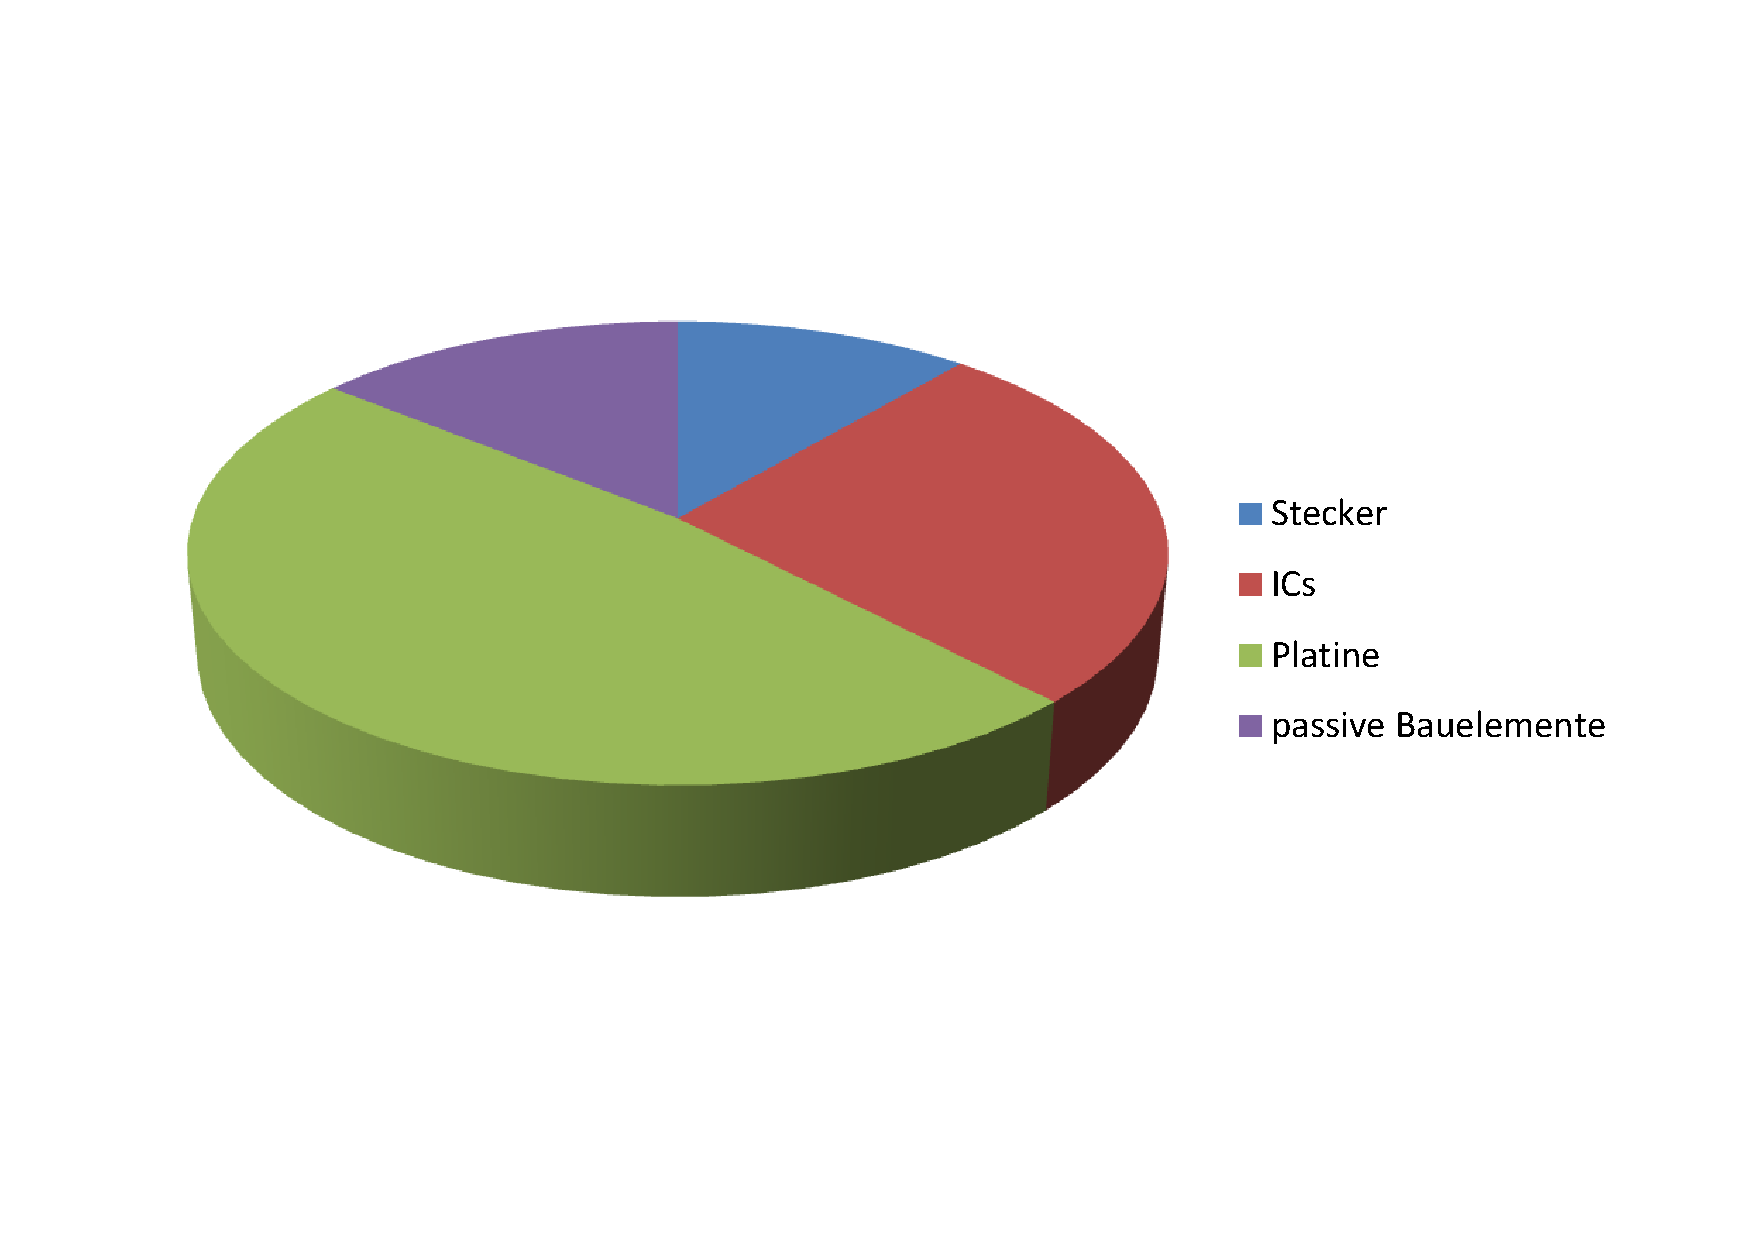
\includegraphics[width=\textwidth]{./Bilder/Platinenkosten.pdf}
\end{minipage}
\begin{minipage}[h]{0.5\textwidth}
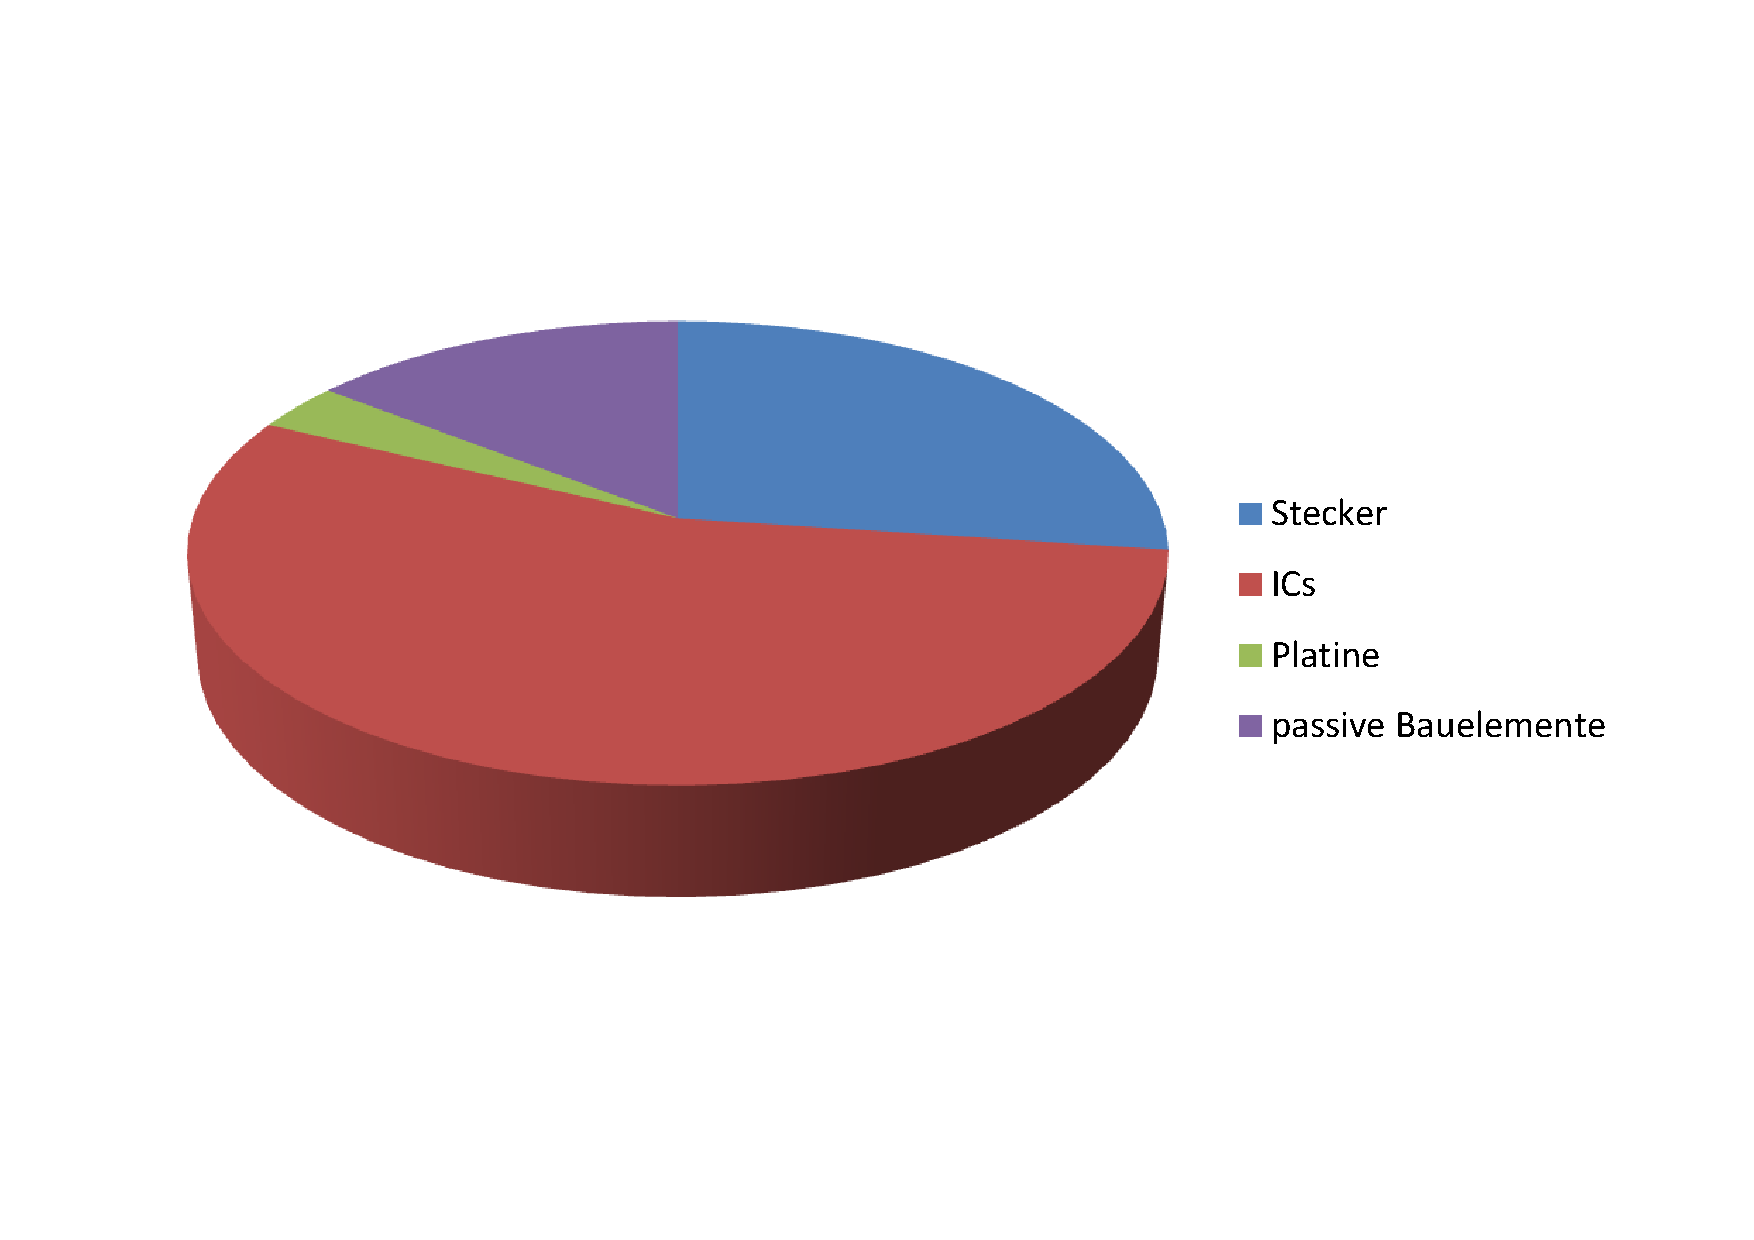
\includegraphics[width=\textwidth]{./Bilder/Platinenkosten-tausend.pdf}
\end{minipage}
\caption{Aufteilung der Kosten für die Stückzahlen 1 (links) und 1000 (rechts)}
	\label{fig:LDO}
\end{figure}

Es ist zu erkennen, dass bei geringen Stückzahlen die Platine ungefähr die Hälfte der Kosten ausmacht, während sie bei hohen Stückzahlen fast gar nicht mehr ins Gewicht fällt. Bei hohen Stückzahlen sind der größte Kostenfaktor die ICs. 



\chapter{Fazit und Ausblick}\label{kap8}
Ziel dieser Arbeit war es, eine eingebettete Elektronik für den linearen Schaltaktor am Prüfstand zu entwickeln und zu testen. Im ersten Schritt wurden dazu die bereits bestehende Hard- und Software der bisher am Prüfstand angebrachten Elektronik analysiert, die Anforderungen an das Endprodukt festgelegt und auf Grundlage dessen schrittweise eigene Schaltungen auf Testboards kreiert und untersucht. Hierfür wurde die Elektronik vor allem in Aktoransteuerung, Recheneinheit und Sensorik unterteilt, welche später auf der Endplatine wieder zusammengeführt wurden. Nachdem die H-Brücke, geschaltet über den Mikrocontroller, erfolgreich den Aktor in Betrieb setzten konnte und die Datenübertragung von Lage- und Temperatursensor mit dem Mikrocontroller sichergestellt werden konnte, wurden anschließend alle Subsysteme kombiniert, sodass ein endgültiger Prototyp entstand, welcher alle Performanceanforderungen erfüllen sollte. Dieser wurde mit Hilfe der parallel erarbeiteten Programmierung in Matlab Simulink durch Verwendung des Waijung Blocksets über den Mikrocontroller gesteuert und die Funktionen überprüft. Auch die Regelung der Schaltgabelposition wurde überarbeitet und optimiert.
Anhand des funktionierenden Prototypen wurde daraufhin die Platine nach einer Einarbeitung in Platinendesign geplant und entworfen. Die industriell gefertigte Platine konnte nun im institutseigenen Lötlabor mit allen Komponenten bestückt werden und im Anschluss am Prüfstand angeschlossen und getestet werden.
Nachdem der Mikrocontroller einmal \textit{geflasht} wird, steht die Funktionalität bei anliegender Versorgungsspannung bereit. Die CAN-Schnittstelle der Platine stellt eine Echtzeitkommunikation mit der MicroAutoBox her, sodass der Aktor über die Benutzeroberfläche ControlDesk am PC gesteuert werden kann. Die H-Brückenschaltung ermöglicht das Ansteuern des Aktors und somit das Schalten des Getriebes in Normalstellung oder einen der beiden Gänge. Der Lagesensor erfasst währenddessen die Position der Schaltgabel, die über die nichtflüchtige Kalibrierung genau berechnet werden kann. Die implementierte Regelung sorgt für die möglichst genaue Einhaltung der Sollvorgabe der Schaltgabelposition.
In der vorliegenden Arbeit konnte eine funktionierende eingebettete Elektronik für den linearen Tauchspulenaktor am Prüfstand des IMS entwickelt werden. Besonders hervorzuheben ist dabei die Kompaktheit der Platine, die direkt am Aktor angebracht wird, gegenüber dem vorherigen Zustand. Schnittstellen sowie Versorgung sind über einen einzigen Steckerausgang verbunden, der wahlweise mit dem passenden Gegenstück zur Programmierung oder zum Betrieb gekoppelt werden kann. \autoref{fig:fazit} zeigt übersichtlich das Ergebnis der Arbeit mit der eingebetteten Elektronik aufgeteilt in ihre Subsysteme, sowie den Schnittstellen zum Aktor, Lagesensor sowie zur MicroAutoBox, welche in der Platinenschaltung integriert wurden. 


\begin{figure}[H]
	\centering
		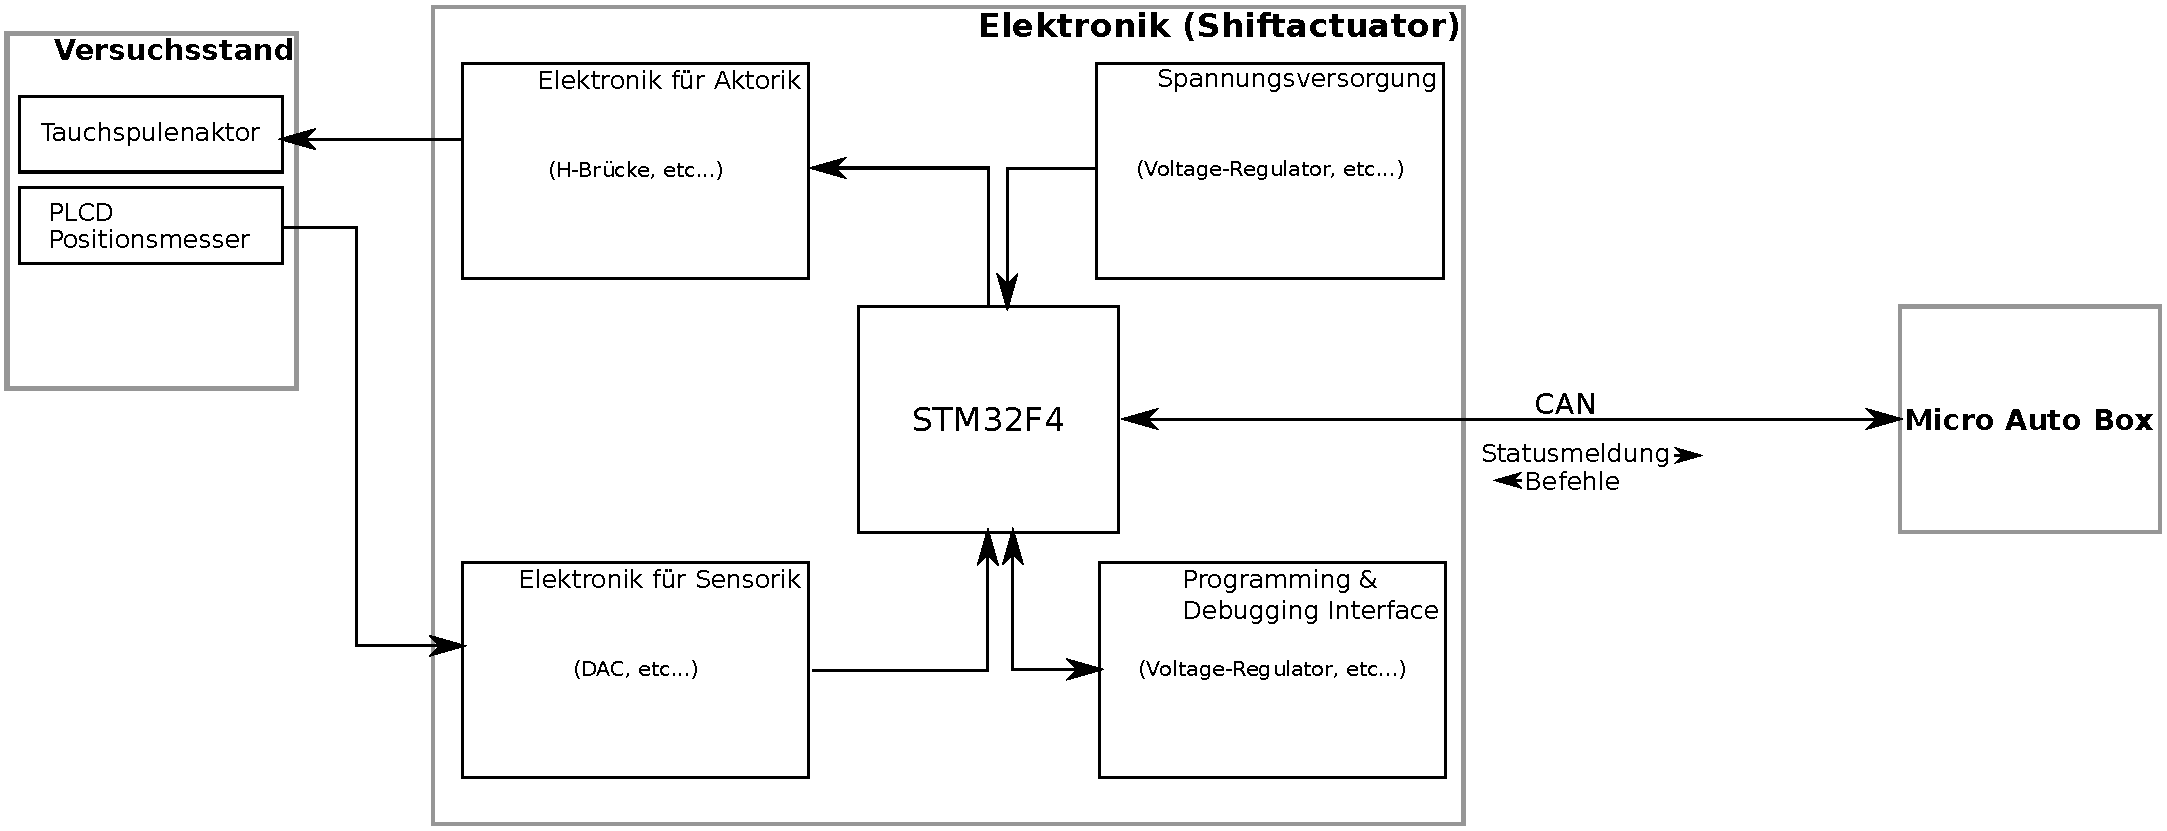
\includegraphics[width=1\linewidth]{Bilder/fazit.pdf}
	\caption{Ergebnis der eingebetteten Elektronik und Schnittstellen}
	\label{fig:fazit}
\end{figure}\noindent

Die gestellten Anforderungen wurden weitestgehend erfüllt (vgl. \autoref{vergleich}), sodass von einem erfolgreichen und zufriedenstellenden Produktdesign ausgegangen werden kann. Eine Weiterentwicklung der eingebetteten Elektronik kann aufgrund der flexiblen Systemintegrierbarkeit und des leicht zu bedienenden Programms in weiteren Arbeiten erfolgen. 

\section{Ausblick} 

Der Schaltaktorikprüfstand des IMS wird stetig weiterentwickelt. So sind auch im Anschluss an diese Projektarbeit weitere Schritte zur Optimierung des Gesamtsystems denkbar und geplant. Zunächst soll der bisher angebrachte Aktor durch einen im Wirkprinzip äquivalenten Aktor mit einem Strom von ca. \SI{50}{A} bei maximal anliegender Spannung anstatt den jetzigen ca. \SI{19}{A} bei Maximalspannung ersetzt werden. Diese geplante Neuerung wurde auch in der Komponentenauswahl während dieser Arbeit  berücksichtigt, weshalb die Funktionalität der eingebetteten Elektronik auch weiterhin gegeben sein sollte. Weiterhin geplant ist es, die MicroAutoBox als CAN-Kommunikationspartner langfristig auszutauschen.
Das Mitschwingen des kompletten Prüfstands während den großen Kraftübertragungen eines Schaltvorgangs stellt ein Problem dar, welches die Messungenauigkeiten bedingt. 
Sinnvoll wäre es, die Halterung des PLCD-Sensors zur Erfassung der Schaltgabelposition steifer zu gestalten, um eine optimale Positionsmessung und somit bessere Regelergebnisse zu erreichen. Bisher ist der Sensor leicht beweglich befestigt und kann sich somit schnell verstellen. Eine weitere Lösung für dieses Problem ist der Einsatz einer sensorlosen Positionserfassung, wie sie bereits in einer vorangegangenen Arbeit \cite{adp} theoretisch entwickelt wurde. Damals konnte die Umsetzung noch nicht erfolgen, da das Messverfahren nur auf der MicroAutoBox implementiert war, dessen Abtastrate des AD-Wandlers nicht hoch und die Anstiegsrate der digitalen Ausgänge zur Erzeugung einer PWM-Frequenz nicht schnell genug waren. Der STM32F405RGT7 mit einer ADC Abtastrate von bis zu 6Ms/s im Interleave Mode und einer Ansprechzeit von 125 ns ist laut den gestellten Anforderungen aber ausreichend, um das entwickelte Messverfahren durchzuführen.\\
Wie in \autoref{diskreg} analysiert wäre die Implementierung eines Haltereglers Gegenstand zukünftiger Forschung. Über diesen ließen sich eine Optimierung der Ganghaltung ermöglichen. 


%%%%%%%%%%%%%%%%%%%%%%%%%%%%%%%%%%%%%%%%%%

\listoffigures\addcontentsline{toc}{chapter}{\listfigurename}
\end{document}
